\documentclass[11pt,a4paper,notitlepage,fleqn,final]{article}

\usepackage{amsmath}
\usepackage{amsfonts}
\usepackage{amssymb}
\usepackage{libs/commath2}
\usepackage[table]{xcolor}
\usepackage[hidelinks]{hyperref}
\usepackage[skins,theorems]{tcolorbox}
\usepackage{titlesec}
\usepackage{circuitikz}
\usepackage{pgfplots}
\usepackage{mathtools}
\usepackage[makeroom]{cancel}
\usepackage{mathrsfs}
\usepackage{wrapfig}
\usepackage{subcaption}
\usepackage{floatrow}
\usepackage{esint}
\usepackage{enumitem}
\usepackage{bm}
\usepackage{relsize}
\usepackage{xfrac}
\usepackage{comment}
\usepackage{siunitx}
\usepackage{MnSymbol}
\usepackage[obeyDraft]{todonotes}
\usepackage[linesnumbered,lined]{algorithm2e}


\pgfplotsset{compat=1.13}
\usetikzlibrary{arrows.meta}
\usetikzlibrary{patterns}
\usetikzlibrary{decorations.pathmorphing,patterns}
\usetikzlibrary{decorations.markings}
\usetikzlibrary{backgrounds}
\usetikzlibrary{shapes.misc}
\usetikzlibrary{shapes.multipart}
\usetikzlibrary{shadows.blur}
\usetikzlibrary{snakes}
\usetikzlibrary{fadings}
\usetikzlibrary{intersections}
\usetikzlibrary{arrows.meta}
\usetikzlibrary{calc}
\usetikzlibrary{matrix}

\tcbuselibrary{breakable}

\tikzset{cross/.style={cross out, draw,
        minimum size=2*(#1-\pgflinewidth),
        inner sep=0pt, outer sep=0pt}}
\tikzset{
    mark position/.style args={#1(#2)}{
        postaction={
            decorate,
            decoration={
            	post length=1mm, % ??? Magic to fix "Dimension
            	pre length=1mm, % ???  too large" errors.
                markings,
                mark=at position #1 with \coordinate (#2);
            }
        }
    }
}

\pgfmathdeclarefunction{sinc}{1}{%
	\pgfmathparse{abs(#1)<0.01 ? int(1) : int(0)}%
	\ifnum\pgfmathresult>0 \pgfmathparse{1}\else\pgfmathparse{sin(#1 r)/#1}\fi%
}
\pgfmathdeclarefunction{gauss}{2}{%
	\pgfmathparse{1/(#2*sqrt(2*pi))*exp(-((x-#1)^2)/(2*#2^2))}%
}

\usepackage[left=2cm,right=2cm,top=2cm,bottom=2cm]{geometry}

%\usepackage[no-math]{fontspec}
\usepackage{fontspec}
%\usepackage{mathspec}
\usepackage{unicode-math}
\setmainfont{texgyretermes-regular.otf}
\setsansfont{texgyreheros-regular.otf}
%\newfontfamily\greekfont[Script=Greek]{Linux Libertine O}
%\newfontfamily\greekfontsf[Script=Greek]{Linux Libertine O}
\usepackage{polyglossia}
\newfontfamily\greekfont[Script=Greek]{texgyretermes-regular.otf}
\newfontfamily\greekfontsf[Script=Greek]{texgyreheros-regular.otf}
\newfontfamily\greekfonttt[Script=Greek]{Latin Modern Mono}
%\usepackage[greek]{babel}
\setdefaultlanguage{greek}
\setotherlanguage{english}
\newcommand{\textlatin}[1]{#1}
%\newcommand{\mathlarger}{}

%\usepackage[utf8]{inputenc}
%\usepackage[greek]{babel}


%\usepackage{tkz-euclide} % loads  TikZ and tkz-base
%\usetkzobj{angles} % important you want to use angles

\newlist{enumparen}{enumerate}{1}
\setlist[enumparen]{label=(\arabic*)}
\newlist{enumpar}{enumerate}{1}
\setlist[enumpar]{label=\arabic*)}

\newlist{enumgreek}{enumerate}{1}
\setlist[enumgreek]{label=\alph*.}
\newlist{enumgreekparen}{enumerate}{1}
\setlist[enumgreekparen]{label=(\alph*)}
\newlist{enumgreekpar}{enumerate}{1}
\setlist[enumgreekpar]{label=\alph*)}


\newlist{enumroman}{enumerate}{1}
\setlist[enumroman]{label=(\roman*)}

\newlist{enumlatin}{enumerate}{1}
\setlist[enumlatin]{label=(\alph*)}

\newlist{invitemize}{itemize}{1}
\setlist[invitemize]{noitemsep,label=}

\usepackage{letltxmacro}

\LetLtxMacro\OriginalLongrightarrow\Longrightarrow
\LetLtxMacro\OriginalLongleftarrow\Longleftarrow

% Implement new macros
% --------------------
\usepackage{trimclip}
\DeclareRobustCommand\Longrightarrow{\NewRelbar\joinrel\Rightarrow}
\DeclareRobustCommand\Longleftarrow{\Leftarrow\joinrel\NewRelbar}

\makeatletter
\DeclareRobustCommand\NewRelbar{%
  \mathrel{%
    \mathpalette\@NewRelbar{}%
  }%
}
\newcommand*\@NewRelbar[2]{%
  % #1: math style
  % #2: unused
  \sbox0{$#1=$}%
  \sbox2{$#1\Rightarrow\m@th$}%
  \sbox4{$#1\Leftarrow\m@th$}%
  \clipbox{0pt 0pt \dimexpr(\wd2-.6\wd0) 0pt}{\copy2}%
  \kern-.2\wd0 %
  \clipbox{\dimexpr(\wd4-.6\wd0) 0pt 0pt 0pt}{\copy4}%
}
\makeatother


\makeatletter
\pgfdeclareradialshading[tikz@ball]{ball}{\pgfqpoint{0bp}{0bp}}{%
	color(0bp)=(tikz@ball!50!white);
	color(10bp)=(tikz@ball!50!white);
	color(15bp)=(tikz@ball!70!black);
	color(20bp)=(black!70);
	color(30bp)=(black!70)}%
\makeatother


\makeatletter
\let\anw@true\anw@false

%\newcommand{\attnboxed}[1]{\textcolor{red}{\fbox{\normalcolor\m@th$\displaystyle#1$}}}
\makeatother
\tcbset{highlight math style={enhanced,colframe=red,colback=white,%
        arc=0pt,boxrule=1pt,shrink tight,boxsep=1.5mm,extrude by=0.5mm}}
\newcommand{\attnboxed}[1]{\tcbhighmath[colback=red!5!white,drop fuzzy shadow,arc=0mm]{#1}}
\titleformat{\section}{\bf\Large}{Κεφάλαιο \thesection}{1em}{}
\newtcolorbox{attnbox}[1]{colback=red!5!white,%
    colframe=red!75!black,fonttitle=\bfseries,title=#1}
\newtcbox{quickattnbox}[1]{colback=red!5!white,%
	colframe=red!75!black,fonttitle=\bfseries,title=#1}
\newtcolorbox{infobox}[1]{colback=blue!5!white,%
    colframe=blue!75!black,fonttitle=\bfseries,title=#1}

\AtBeginDocument{%
\let\arg\relax
\let\Re\relax
\let\Im\relax
\DeclareMathOperator{\arg}{Arg}
\DeclareMathOperator{\Re}{Re}
\DeclareMathOperator{\Im}{Im}
}
\DeclareMathOperator{\sinc}{sinc}
\DeclareMathOperator{\sgn}{sgn}
\DeclareMathOperator{\erf}{erf}
\DeclareMathOperator{\cov}{cov}

\newif\ifhidetikz
\hidetikzfalse
%\hidetikztrue   % <---- comment/uncomment that line

\ifhidetikz

\let\oldtikzpicture\tikzpicture
\let\oldendtikzpicture\endtikzpicture

\renewenvironment{tikzpicture}{
    \tiny
    \tt
    \color{blue}
    \newcommand{\draw}{\textit{draw}}
    \newcommand{\filldraw}{\textit{filldraw}}
    %\newcommand{\x}{\textit{x}}
    %\newcommand{\p}{\textit{x}}
    \newcommand{\x1}{\textit{x1}}
    \newcommand{\y1}{\textit{y1}}
    \newcommand{\p1}{\textit{p1}}
}{
}
\newenvironment{axis}{
    \newcommand{\addplot}{\textit{addplot}}
}{
}
\fi

\newcommand{\nesearrow}{%
	\,%
	\smash{\raisebox{-1.1ex}
		{$%
			\stackrel{\displaystyle\nearrow}{\displaystyle\searrow}%
			$}}%
}
\newcommand{\degree}{^{\circ}} % not great

\newtcbtheorem[number within=section]{theorem}{Θεώρημα}%
{colback=green!5,colframe=green!35!black,colbacktitle=green!35!black,fonttitle=\bfseries,enhanced,attach boxed title to top left={yshift=-2mm,xshift=-7mm},width=.9\textwidth,arc=.7mm}{th}
\newtcbtheorem[number within=section]{defn}{Ορισμός}%
{colback=blue!5,colframe=cyan!35!black,colbacktitle=blue!35!black,fonttitle=\bfseries,enhanced,attach boxed title to top left={yshift=-2mm,xshift=-2mm}}{def}
\newtcbtheorem[number within=section]{exercise}{Άσκηση}%
{colback=gray!3,colframe=gray!35!black,colbacktitle=gray!35!black,fonttitle=\bfseries,enhanced,attach boxed title to top left={yshift=-2mm,xshift=-2mm}}{exc}




\title{Στοχαστικό Σήμα
	\\
	{
	\normalsize Σημειώσεις από τις παραδόσεις
	}}
\date{2017
	\\
	{
	\small Τελευταία ενημέρωση: \today
	}
	}
\author{
	Για τον κώδικα σε \LaTeX, ενημερώσεις και προτάσεις:
\\
 \url{https://github.com/kongr45gpen/ece-notes}}

\setmainfont{Linux Libertine O}
\setsansfont{Ubuntu}
%\newfontfamily\greekfont[Script=Greek]{Linux Libertine O}
%\newfontfamily\greekfontsf[Script=Greek]{Linux Libertine O}
\usepackage{polyglossia}
\newfontfamily\greekfont[Script=Greek,Scale=0.95]{GFS Artemisia}


\begin{document}
	\maketitle

	\tableofcontents

	\newpage

	\setcounter{section}{-1}
	\section{Εισαγωγή}

    \textbf{Στοχαστικό σήμα} - δεν σημαίνει στοχάζομαι
    (σκέφτομαι), αλλά
    τυχαίο σήμα

    \paragraph{Ντετερμινιστικό σήμα}
    \( A_c\cos(2\pi f t + \sfrac{\pi}{2}) \)

    \begin{tikzpicture}[scale=1.2]


    \draw (0,-1) -- (0,1);
    \draw[->] (-0.5,0) -- (2.6,0);

    \draw[very thick,xscale=0.5,yscale=0.7,samples=50,domain=0:5,smooth,variable=\x,blue]
    plot ({\x},{sin(pi*\x r)});
    \end{tikzpicture}

    Για κάθε χρόνο \(t\) μπορούμε να βρούμε την τιμή του
    σήματος.

    Αν γνωρίζουμε τα πάντα για
    την αρχική κατάσταση ενός συστήματος
    (π.χ. του σύμπαντος), μπορούμε να προβλέψουμε
    (ίσως με δυσκολία) κάθε επόμενη κατάστασή του.

    Οι περισσότερες διαδικασίες στη φύση είναι τυχαίες.

    \paragraph{Διαδικαστικά}
    Το μάθημα γίνεται σε δύο τμήματα μόνο από τον κ. Δημάκη. Το
    ένα τμήμα της Τρίτης θα μεταφερθεί στο μεσημέρι της Πέμπτης.

    Ασκήσεις και λύσεις τους θα αποστέλλονται στο e-mail.

    \paragraph{}
    \begin{itemize}
    	\item Ένα σκυλί δάγκωσε έναν άνθρωπο στο δρόμο
    	\( \leftarrow \) δεν είναι πληροφορία, επειδή έχει
    	μεγάλη πιθανότητα να συμβεί.
    	\item Ένας άνθρωπος δάγκωσε έναν σκύλο στο δρόμο
    	\( \leftarrow \) είναι πληροφορορία, επειδή έχει μικρή
    	πιθανότητα.
    \end{itemize}

    \section{Θεωρία Πιθανοτήτων}
    Ασχολείται με τυχαία γεγονότα, δηλαδή γεγονότα το αποτέλεσμα
    των οποίων:
    \begin{itemize}
    	\item Δεν μπορούμε να προβλέψουμε
    	\item Δεν μπορούμε να καταλάβουμε ή
    	\item Έχει πάρα πολλά στοιχεία που το επηρεάζουν
    \end{itemize}
    και πειράματα τα οποία όταν επαναλαμβάνουμε βγάζουν
    διαφορετικό αποτέλεσμα στις ίδιες συνθήκες (π.χ. ρίψη
    ζαριού, σε αντίθεση με το μήλο του Νεύτωνα).

    Επομένως στα πειράματα τύχης \textbf{δεν μπορεί να
    προβλεφθεί ακριβώς η έξοδος}.

	\paragraph{Ορισμός Πιθανότητας από Laplace}
	\hspace{0pt}

	    
\begin{tikzpicture}[scale=1.2]

	    \filldraw[fill=green!20,draw=black!70!green,very thick] plot [smooth cycle]
	    coordinates {(0.8,1) (1.5,1.7) (2,1.5) (2.6,1.5) (2.5,0.8) (1.9, 0.6) (1.6,0.3) (1.2,0.2) (0.6, 0.7)};

	    \draw (0,0) rectangle (2.7,2.2) node[below left] {$N$};
	    \filldraw (1,1) circle(1pt) node[above right] {$1$};
	    \filldraw (1.5,1.2) circle(1pt) node[above right] {$2$};
	    \filldraw (0.2,0.4) circle(1pt) node[above right] {$3$};
	    \filldraw (2,1.1) circle(1pt) node[above right] {$4$};
	    \filldraw (1.3,0.3) circle(1pt) node[above right] {$5$};
	    \filldraw (2.1,0.4) circle(1pt) node[below right] {$6$};
	    \filldraw (0.3,1.7) circle(1pt) node[above right] {$7$};
	    \filldraw (0.5,1.1) circle(1pt) node[above right] {$8$};

	    \draw[->,blue!30!black] (0.2,1.7) to[bend left=45] (-0.5, 2.2) node[above] {ισοπίθανα ενδεχόμενα};
	    \draw[->,green!30!black] (0.8,0.35) to[bend right=85] (0.5, -1) node[right] {γεγονός};

	    \end{tikzpicture}
	\[
	P(A) = \frac{N_A}{N}
	\]
	Ο ορισμός έχει τα προβλήματα:
	\begin{itemize}
		\item Δεν αντιστοιχεί σε πραγματικό πείραμα τύχης
		\item Είναι κυκλικός (ορίζει την πιθανότητα με βάση
		ισο\underline{πίθανα} ενδεχόμενα)
	\end{itemize}
	\paragraph{Ορισμός Πιθανότητας von Mises}
	Εκτελούμε ένα πείραμα τύχης με \(N\) επαναλήψεις. Αν ένα
	γεγονός συμβεί \(N_A\) φορές, τότε
	\[
	P(A) = \lim_{N\to  \infty } \frac{N_A}{N}
	\]
	Όμως είναι δύσκολο να χρησιμοποιηθεί επειδή αντιστοιχεί σε
	πραγματικό πείραμα.
	\paragraph{Ιδιότητες που προκύπτουν από
		τους παραπάνω ορισμούς}
	\begin{enumroman}
		\item \( 0 \leq P(A) \leq 1 \)
		\item \( S \text{ δειγματικός χώρος } \quad
		P(S) = 1 \)
		\item \( P(A\cup B) = P(A+B) = P(A \text{ ή } B)
		= P(A) + P(B) \qquad (A,B \text{ ασυμβίβαστα})
		 \)
	\end{enumroman}

	\subsection{Αξιωματικός ορισμός της πιθανότητας
		Wiener - Kolmogorov}

	\textbf{Πείραμα} είναι κάθε νοητική ή φυσική διεργασία,
	με την οποία
	συνδέουμε μία πράξη με κάποιο αποτέλεσμα.

	Κάθε εκτέλεση του πειράματος ονομάζεται \textbf{δοκιμή}

	Ένα πείραμα έχει έναν δειγματικό χώρο με όλα τα δυνατά
	αποτελέσματά του:
	\[
	S = \left\lbrace J_1,J_2,\dots,J_n \right\rbrace
	\]

	Ένα \textbf{γεγονός} είναι ένα από τα \( 2^n \) δυνατά
	υποσύνολα του \(S\): \[ A \subseteq S \]
	\paragraph{Ορισμός}
	\( A \to P(A) \)
	\begin{enumroman}
		\item \( P(A) \geq 0 \)
		\item \( P(S) = 1 \)
		\item αν \( A \cap B = 0 \), τότε \( P(A \cup B)
		= P(A)+P(B) \)
	\end{enumroman}

	Ο ορισμός αυτός δεν μας δίνει συγκεκριμένη τεχνική υπολογισμού
	πιθανοτήτων, επομένως μπορούμε να χρησιμοποιήσουμε οποιαδήποτε
	τεχνική (π.χ. Laplace) θέλουμε.


	\def\boundingbox{(-2cm,-2cm) rectangle (4cm,2cm)}
	\colorlet{circle edge}{blue!50}
	\colorlet{circle area}{blue!20}
	\tikzset{filled/.style={fill=circle area, draw=circle edge, thick},
		outline/.style={draw=circle edge, thick}}

	\subsection{Ιδιότητες}
	\begin{enumpar}
		\item \( A = B \implies P(A)=P(B) \) \\
		\item \( P(\emptyset) = 0 \)
		\item Αφού \( A\cdot\bar A = \emptyset \quad
		A+\bar A = S \), τότε:
		\begin{align*}
			P(A+\bar A) = P(S) = 1 & \quad P(\bar A) = 1 - P(A) \\
			P(A) + P(\bar A) = 1
		\end{align*}
		\item Αν \( A \cdot B \neq \emptyset \), τότε
		\[
		P(A+B) = P(A) + P(B) - P(A\cdot B) \leq 1
		\]
		\begin{tikzpicture}[scale=0.65]
		\def\firstcircle{(0,0) circle (1.5cm)}
		\def\secondcircle{(0:2cm) circle (1.5cm)}
		\begin{scope}
		\clip \firstcircle;
		\fill[filled] \secondcircle;
		\end{scope}
		\draw[outline] \firstcircle node {$A$};
		\draw[outline] \secondcircle node {$B$};
		\draw \boundingbox;
		\draw (1,0) node[scale=0.6] {$A\cap B$};
		\end{tikzpicture}

		\subparagraph{Απόδειξη}
		\begin{align*}
			A+B &= A+ \bar A \cdot B \\
			B &= A\cdot B + \bar A \cdot B \\
			P(A+B) &= P(A) + P(\bar A \cdot B) \\
			P(B) &= P(A\cdot B) + P(\bar A \cdot B)\\
			P(A+B) &= P(B)+P(A) -P(AB)
		\end{align*}
		\item \( A \subseteq B \implies P(A) \leq P(B) \)

		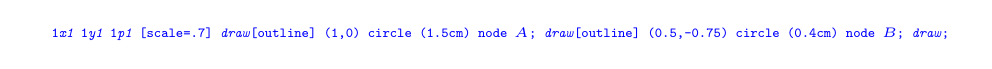
\begin{tikzpicture}[scale=.7]
		\draw[outline] (1,0) circle (1.5cm) node {$A$};
		\draw[outline] (0.5,-0.75) circle (0.4cm) node {$B$};
		\draw \boundingbox;
		\end{tikzpicture}

		\begin{align*}
			\intertext{επειδή}
			B &= A + \bar A \cdot B \\
			P(B) &= P(A) + P(\bar A\cdot B) \geq P(A)
		\end{align*}

		\item Υπό συνθήκη πιθανότητα
		\[
		P(A/B) = \frac{P(AB)}{P(B)}
		\]

		\begin{tikzpicture}
		\filldraw (-0.1,0) circle (1.5pt);
		\draw (0,0) node[below right,yshift=2.5mm,rectangle,align=left]
		{Αν $A\cdot B=\emptyset$\\$P(A/B)=0$};
		\begin{scope}[xshift=5cm,yshift=3mm]
		\draw (0,0) rectangle (-1.5,-1);
		\draw[fill=blue,fill opacity=0.2] (-0.375,-0.5) circle (2.5mm);
		\draw[fill=blue,fill opacity=0.2] (-1.125,-0.5) circle (2.5mm);
		\draw (-0.8,-0.2) node[scale=.8] {$A$};
		\draw (-0.13,-0.2) node[scale=.8] {$B$};
		\draw (-1.3,0) arc(360:270:0.2) node[xshift=0.8mm,yshift=1.1mm,scale=.5] {$S$};
		\end{scope}

		\begin{scope}[yshift=-1.5cm]
		\filldraw (-0.1,0) circle (1.5pt);
		\draw (0,0) node[below right,yshift=2.5mm,rectangle,align=left]
		{Αν $A\subset B$\\$A\cdot B = A$\\$P(A/B)=\frac{P(A)}{P(B)}$};
		\begin{scope}[xshift=5cm,yshift=3mm]
		\draw (0,0) rectangle (-1.5,-1);
		\draw[fill=blue,fill opacity=0.2] (-0.75,-0.5) circle (4mm);
		\draw[fill=blue,fill opacity=0.2] (-0.75,-0.5) circle (1.5mm);
		\draw (-0.75,-0.5) node[scale=.7] {$A$};
		\draw (-0.25,-0.2) node[scale=.8] {$B$};
		\draw (-1.3,0) arc(360:270:0.2) node[xshift=0.8mm,yshift=1.1mm,scale=.5] {$S$};
		\end{scope}
		\end{scope}

		\begin{scope}[yshift=-3.5cm]
		\filldraw (-0.1,0) circle (1.5pt);
		\draw (0,0) node[below right,yshift=2.5mm,rectangle,align=left]
		{Αν $A\supset B$\\$A\cdot B = B$\\$P(A/B)=\frac{P(B)}{P(B)}=1$};
		\begin{scope}[xshift=5cm,yshift=3mm]
		\draw (0,0) rectangle (-1.5,-1);
		\draw[fill=blue,fill opacity=0.2] (-0.75,-0.5) circle (4mm);
		\draw[fill=blue,fill opacity=0.2] (-0.75,-0.5) circle (1.5mm);
		\draw (-0.75,-0.5) node[scale=.7] {$B$};
		\draw (-0.25,-0.2) node[scale=.8] {$A$};
		\draw (-1.3,0) arc(360:270:0.2) node[xshift=0.8mm,yshift=1.1mm,scale=.5] {$S$};
		\end{scope}
		\end{scope}

		\begin{scope}[xshift=5cm,yshift=2cm]
		\draw (0,0) rectangle (-1.5,-1);
		\draw[fill=blue,fill opacity=0.2] (-0.6,-0.5) circle (3mm);
		\draw[fill=blue,fill opacity=0.2] (-0.9,-0.5) circle (3mm);
		\draw (-1.33,-0.5) node[scale=.8] {$A$};
		\draw (-0.17,-0.5) node[scale=.8] {$B$};
		\draw (-1.3,0) arc(360:270:0.2) node[xshift=0.8mm,yshift=1.1mm,scale=.5] {$S$};
		\end{scope}
		\end{tikzpicture}

		\item \begin{tikzpicture}[baseline=(current bounding box.north)]
		\draw (0,0) rectangle (4,2);

		\draw[orange,fill=orange!50!white] (2,1) circle (0.8cm);

		\draw plot [smooth,tension=1] coordinates {(0.6,2) (1.5,1.6) (2,1.3) (2.5,1.6) (3.4,2)};
		\draw plot[smooth,tension=1.5] coordinates {(0.4,0) (2,0.9) (3.6,0)};
		\draw plot[smooth,tension=2] coordinates {(2,1.3) (2.1,1.1) (2,0.9)};

		\draw[brown!50!black] (0,1.7) arc (270:360:0.3);
		\draw[brown!50!black] (0.12,1.87) node {$\mathsmaller{S}$};

		\draw (2,1.7) node {$A_1$};
		\draw (3.4,1.1) node {$A_2$};
		\draw (2,0.4) node {$A_3$};
		\draw (0.8,1.1) node {$A_4$};

		\draw[orange!70!black] (2.85,0.35) node {$B$};

		\end{tikzpicture}

		Έστω ένας διαμερισμός του δειγματικού χώρου και ένα
		ενδεχόμενο \( B \) αυτού, δηλαδή:
		\begin{gather*}
			A_1+A_2+A_3+A_4 = S \\
			A_i A_j = \emptyset \ \forall i,j \\[.3ex]
			(B \cdot A_i) \cdot (B \cdot A_j) = \emptyset
		\end{gather*}

		Τότε:
		\begin{align*}
			B &= B\cdot S = B(A_1+A_2+A_3+A_4) \\
			B &= B\cdot A_1 + B\cdot A_2 + B\cdot A_3 + B\cdot A_4 \\
			P(B) &= P(BA_1) + P(BA_2) + P(BA_3) + P(BA_4)
			\intertext{\( P(B/A_i) = \frac{P(B)\cdot A_i}{P(A_i)} \)}
			\intertext{\( P(BA_i) = P(B/A_i)\cdot P(A_i) \)}
			P(B) &= P(B/A_1)P(A_1)+P(B/A_2)P(A_2)+P(B/A_3)P(A_3)
			+P(B/A_4)P(A_4)
		\end{align*}

		Το παραπάνω (\textbf{θεώρημα ολικής πιθανότητας})
		εκφράζεται γενικά ως εξής:
		\[
		P(B) = \sum_{i=1}^{m} P(A_i)P(B/A_i)
		\]
		\item
		Από την παραπάνω ιδιότητα έχουμε:
		\begin{align*}
			P(A_iB) &= P(B)P(A_i/B) = P(A_i)P(B/A_i) \\
			P(A_i/B) &= \frac{P(B/A)P(A_i)}{P(B)} \\
			\Aboxed{
     			P(A_i/B) &=
     			\frac{P(B/A_i)P(A_i)}{\displaystyle\sum_{i=1}^{n}P(A_i)P(B/A_i)}
     		} \qquad \text{\textbf{Θεώρημα Bayes}}
		\end{align*}
	\end{enumpar}

	\paragraph{Παράδειγμα}
	\hspace{0pt}

	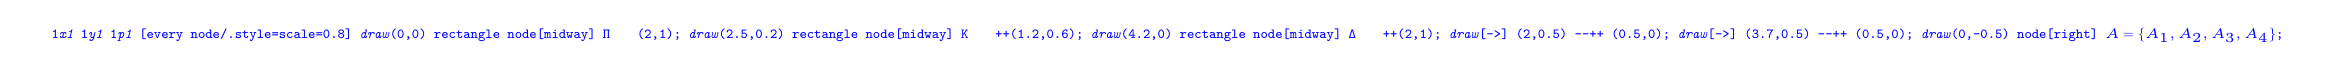
\begin{tikzpicture}[every node/.style={scale=0.8}]
	\draw (0,0) rectangle node[midway] {Πομπός} (2,1);
	\draw (2.5,0.2) rectangle node[midway] {Κανάλι} ++(1.2,0.6);
	\draw (4.2,0) rectangle node[midway] {Δέκτης} ++(2,1);

	\draw[->] (2,0.5) --++ (0.5,0);
	\draw[->] (3.7,0.5) --++ (0.5,0);

	\draw (0,-0.5) node[right] {$A=\lbrace A_1,A_2,A_3,A_4\rbrace$};
	\end{tikzpicture}

	Η είσοδος μπορεί να είναι ένα αλφάβητο \( A \):
	\begin{align*}
		A &= \left\lbrace A_1,A_2,A_3,A_4 \right\rbrace
		\intertext{με πιθανότητες για το καθένα:}
		\Pi_A &= \left\lbrace
		\Pi_{A_1},\Pi_{A_2},\Pi_{A_3},\Pi_{A_4}
		 \right\rbrace
	\end{align*}

	Το κανάλι ποτέ δεν θα μεταφέρει ακριβώς την πληροφορία, αλλά θα
	την μεταβάλλει με κάποιον τρόπο (π.χ. θόρυβος). Αν \( B \) είναι το
	αλφάβητο εξόδου, έχουμε:
	\begin{align*}
	B &= \left\lbrace B_1,B_2,B_3,B_4 \right\rbrace \\
	\Pi_B &= \left\lbrace
	\Pi_{B_1},\Pi_{B_2},\Pi_{B_3},\Pi_{B_4}
	\right\rbrace
	\end{align*}

	Για να μελετήσουμε το κανάλι, μπορούμε να βάλουμε κάποιον να μετράει
	τις πιθανότητες εμφάνισης κάποιας εξόδου με δεδομένη είσοδο (για
	παράδειγμα, να στείλουμε 100\,000 φορές την είσοδο \( A_1 \), και
	να μετρήσουμε πόσες φορές εμφανίζεται η κάθε έξοδος). Έτσι έχουμε
	τις υπό συνθήκη (\textbf{a posteriori}) πιθανότητες:
	\[
	\Pi_{B/A} = \begin{cases}
	\Pi(B_1/A_1),\ \Pi(B_1/A_2),\ \Pi(B_1/A_3), \dots \\
	\Pi(B_2/A_1),\ \Pi(B_2/A_2),\ \dots \\
	\vdots
	\end{cases}
	\]

	Από τις παραπάνω ιδιότητες έχουμε:
	\[
	P(B_1) = P(A_1)P(B_1/A_1)
	+P(A_2)P(B_1/A_2)
	+P(A_3)P(B_1/A_3)
	+P(A_4)P(B_1/A_4)
	\]
	Άρα:
	\[
%	\mathlarger{
		P(A_i/B_j) = \frac{P(B_j/A_i)P(A_i)}{
			\sum_{i=1}^n P(A_i)P(B_j/A_i)
			}
%		}
	\]

	Έτσι, για κάθε έξοδο, μπορούμε να υπολογίσουμε την πιθανότητα
	να προέρχεται από μια είσοδο.

	Αν π.χ. έχουμε: \begin{align*}
		P(A_1/B_4) &= 70\% \\
		P(A_2/B_4) &= 15\% \\
		P(A_3/B_4) &= 8\% \\
		P(A_4/B_4) &= 7\%
	\end{align*}
	μπορούμε να φανταστούμε ότι η έξοδος \( B_4 \) αντιστοιχεί με
	μεγαλύτερη πιθανότητα σε είσοδο \( A_1 \), σύμφωνα με το κριτήριο
	\textbf{MAP} (\textit{maximum a-posteriori probability}).

	Είναι συχνό βέβαια να μη γνωρίζουμε τις \todo{a-priori?}
	πιθανότητες \( P(A_i) \), οπότε μπορούμε να καταφύγουμε σε κόλπα,
	όπως να θεωρήσουμε ότι τα ενδεχόμενα της εισόδου είναι ισοδύναμα.

	\subsubsection{Σήματα}
	\hspace{0pt}

	\begin{tikzpicture}[scale=1.3]
	\fill[cyan!40,path fading=north] (-1,1.125) rectangle (8,2);
	\fill[cyan!40,path fading=south] (-1,-1.125) rectangle (8,-2);
	\fill[green,opacity=.15] (-1,1.125) rectangle (8,0);
	\fill[yellow,opacity=.2] (-1,-1.125) rectangle (8,0);

	\draw[dashed] (-1,1.125) -- (8,1.125);
	\draw[dashed] (-1,-1.125) -- (8,-1.125);

	\draw (-1,0) -- (8,0);
	\draw (0,-2) -- (0,2);
	\def\1{1.5};
	\def\2{0.75}
	\def\3{-0.75}
	\def\4{-1.5}

	\draw (-0.1,\1) node[left,scale=.7] {$1$} -- (0.1,\1);
	\draw (-0.1,\2) node[left,scale=.7] {$2$} -- (0.1,\2);
	\draw (-0.1,\3) node[left,scale=.7] {$3$} -- (0.1,\3);
	\draw (-0.1,\4) node[left,scale=.7] {$4$} -- (0.1,\4);

	\draw (-1.5,\1) node {$a$};
	\draw (-1.5,\2) node {$b$};
	\draw (-1.5,\3) node {$c$};
	\draw (-1.5,\4) node {$d$};
	\draw (-0.8,\1) node[scale=.6] {$\mathtt{11}$};
	\draw (-0.8,\2) node[scale=.6] {$\mathtt{10}$};
	\draw (-0.8,\3) node[scale=.6] {$\mathtt{01}$};
	\draw (-0.8,\4) node[scale=.6] {$\mathtt{00}$};

	\draw[very thick,black] plot [const plot] coordinates
	{(0,\2) (1,\4) (2,\1) (3,\2) (4,\3) (5,\2) (6,\4) (7,\1) (8.1,\1)}
	node[above right] {αρχικό σήμα};

	\foreach \x in {1,2,3,...,5} {
		\draw[draw=gray] (\x,-0.1) -- (\x,0.1) node[midway,below left,scale=.6] {$\x T$};
	}
	\draw (6,0) node[below left,scale=.6] {$\cdots$};

	\draw[very thick,orange!70!brown] plot [smooth,tension=.2] coordinates
	{(0,0) (0.15,0.4) (0.3,1.05) (0.4,1.1) (0.5,1) (0.6,1.10)
		(0.7,1+rand/5) (1,rand/10) (1.2,-1.5+rand/3) (1.4,-1.5+rand/4) (1.5,-1.5+rand/5)
		(1.6,-1.5+rand/4) (1.8,-1.5+rand/2) (1.9,-0.75+rand/2) (2,rand/5) (2.1,0.7+rand/3)
		(2.2,1.2+rand/3) (2.4,1.5+rand/5) (2.6,1.5+rand/5) (2.7,1.2+rand/6) (2.9,1+rand/5)
		(3.1, 0.7+rand/4) (3.3, 0.8+rand/5) (3.4, 0.8+rand/4) (3.6,0.5+rand/3) (3.8,0.9+rand/4)
		(4,1+rand/4) (4.1,rand/4) (4.2, 0.4+rand/4) (4.3, -0.3+rand/3) (4.4, -0.5+rand/4)
		(4.5,-0.5+rand/5) (4.6,-0.5+rand/6) (4.8,-0.3+rand/4) (5,0+rand/4) (5.2,0.3+rand/4)
		(5.4,0.6+rand/4) (5.6,1+rand/4) (5.8,0.8+rand/4) (5.9,rand/4) (6,rand/7)
		(6.2,-0.2+rand/4) (6.4,-1.3+rand/4) (6.6, -0.5+rand/5) (6.8,0.5+rand/3)
		(7,1+rand/3) (7.2,2+rand/4) (7.4,1.6+rand/4) (7.6,1.3+rand/6) (7.8,1.3+rand/8)
		(8,1.3)} node[below right] {σήμα με θόρυβο};

	\draw[very thick,green!50!black] plot [smooth] coordinates
	{(0,0) (0.3,1) (0.7,1) (1.5,-1.5) (2.5,1.5) (3.6,0.6) (3.9,0.8)
		(4.6,-0.5) (5.6,0.85) (6.4,-1.2) (7.1,1.7) (7.7,1.5) (8,1.4)}
	node[right] {σήμα χωρίς υψηλές συχνότητες};
	\end{tikzpicture}

	Ένα πραγματικό σήμα έχει θόρυβο, όπως φαίνεται στο διάγραμμα.
	Το σήμα που στέλνει ο πομπός είναι το αρχικό καθαρό σήμα, ενώ αυτό που λαμβάνει
	ο δέκτης είναι το \textcolor{orange!70!brown}{σήμα με θόρυβο}. Ο δέκτης μπορεί
	αυτό να το επεξεργαστεί ώστε να πάρει ένα
	\textcolor{green!50!black}{σήμα χωρίς υψηλές συχνότητες}. Για
	να εξάγουμε την αρχική τιμή του σήματος από την είσοδο με θόρυβο,
	μπορούμε να χωρίσουμε τη ζώνη του πλάτους σε διαφορετικές περιοχές,
	και κάθε μία από αυτές να την αντιστοιχούμε σε μία τιμή εξόδου,
	\( \alpha, \beta, \gamma \) ή \( \delta \). Όπως και πριν, κάθε
	είσοδος αντιστοιχεί με διαφορετική πιθανότητα σε κάθε έξοδο:
	\begin{center}
	\begin{tikzpicture}[xscale=1.3]
	\coordinate (a) at (2,6);
	\coordinate (b) at (2,4);
	\coordinate (c) at (2,2);
	\coordinate (d) at (2,0);
	\coordinate (1) at (0,6);
	\coordinate (2) at (0,4);
	\coordinate (3) at (0,2);
	\coordinate (4) at (0,0);

	\draw[green!50!blue!50!white,->] (1.7,6.02) to[bend left] (3.5,7)
	node[right] {$P(1/a)$};

	\draw[green!50!blue!50!white,->] (1.58,5.65) to[bend right] (3.2,6)
	node[right] {$P(2/a)$};

	\draw[green!50!blue!50!white,->] (1.20,4.56) to[bend left=20] (3,5.2)
	node[right] {$P(3/a)$};

	\draw[green!50!blue!50!white,->] (1.36,4.37) to[bend right=20] (3,4.4)
	node[right] {$P(4/a)$};

	\foreach \x in {2,3,4}
	\foreach \y in {a,b,c,d}
	\draw (\x)  to[bend left={5-\x}] (\y);
	\draw (1) to[bend left=4] node[midway,above] {$P(a/1)$} (a);
	\draw (1) to[bend left=4] node[midway,above,sloped] {$P(\beta/1)$}(b);
	\draw (1) to[bend left=4] node[midway,above,sloped] {$\cdots$} (c);
	\draw (1) to[bend left=4] (d);

	\foreach \x in {1,2,3,4}
	\fill (\x) circle (2pt) node[left] {$P_\x \qquad \x$};
	\fill (a) circle (2pt) node[right] {$a$};
	\fill (b) circle (2pt) node[right] {$\beta$};
	\fill (c) circle (2pt) node[right] {$\gamma$};
	\fill (d) circle (2pt) node[right] {$\delta$};
	\end{tikzpicture}
		\end{center}

	\subsubsection{Ανεξαρτησία}
	Δύο γεγονότα λέγονται ανεξάρτητα ανν:
	\[
	P(A\cdot B) = P(A)P(B)
	\]

	Ομοίως ορίζεται η ανεξαρτησία για περισσότερα ενδεχόμενα, ανν:
	\[
	P(A_1A_2\cdots A_n) = P(A_1)P(A_2)\cdots P(A_m)
	\]

	\subsection{Πιθανοτικό Μοντέλο}
	Ένας δειγματικός χώρος \( S \) έχει μεγάλο αριθμό δυνατών υποσυνόλων,
	και στο καθένα από αυτά αντιστοιχεί μία πιθανότητα. Για εμάς μπορεί
	να είναι εύκολο/δυνατό να βρούμε την πιθανότητα μόνο για μερικά
	από αυτά τα υποσύνολα, επομένως ονομάζουμε αυτά γεγονότα, και τα
	τοποθετούμε σε μια τάξη συνόλων \( \mathcal F \), που θα ικανοποιούν:

	\begin{enumroman}
		\item \( \emptyset \in \mathcal F,\
		S \in \mathcal{F}
		 \)
		\item \( A \in \mathcal F \) και το \( \bar A \in \mathcal F \)
		\item \( A \in \mathcal F \) και \( B \in \mathcal F \)
		\( \implies A + B \in \mathcal F \) \quad
		(τότε θα έχουμε και \( A\cdot B,\ A-B \in \mathcal F \))
	\end{enumroman}

	Τότε προκύπτει, αν \( A_1,A_2,\dots,A_n \in \mathcal F \):
	\begin{gather*}
		A_1+A_2+\dots +A_n \in \mathcal F \\
		A_1\cdot A_2 \cdot \cdots \cdot A_n \in \mathcal F
	\end{gather*}

	Το πεδίο \( \mathcal F \) ονομάζεται \textbf{πεδίο Borel}.

	Αν έχουμε τα \( \mathlarger{\mathlarger{(S,\mathcal F,P)}} \),
	δηλαδή το
	δειγματικό χώρο, ένα πεδίο Borel, και τις αντίστοιχες πιθανότητές
	του, τότε έχουμε ένα πλήρες πιθανοτικό μοντέλο.

	\paragraph{Σύνολο με πεπερασμένο αριθμό γεγονότων}
	\begin{align*}
		S &= \left\lbrace J_1,J_2,\dots,J_n \right\rbrace \\
		P_i \to \quad A_1 &=
		\left\lbrace J_i \right\rbrace \in \mathcal F \\
		& P_1+P_2+\dots+P_N = 1 \\
		A &= \left\lbrace J_{k_1},J_{k_2},\dots,J_{k_i} \right\rbrace
		\quad i \leq n \qquad \text{(επιλέγουμε μερικά
			απλά ενδεχόμενα από τον χώρο $S$)} \\
		P(A) &= P\left\lbrace J_{k_1} \right\rbrace +
		P\left\lbrace J_{k_2} \right\rbrace + \dots +
		P\left\lbrace J_{k_i} \right\rbrace \\ &=
		P_{k_1} + P_{k_2} + \dots + P_{k_n}
	\end{align*}

	\paragraph{Σύνολο με πραγματικούς αριθμούς}
	Όταν, για παράδειγμα, περιμένουμε το λεωφορείο στη στάση, ο χρόνος
	\( t \) που πρέπει να περιμένουμε μέχρι να έρθει είναι πραγματικός
	αριθμός:
	\begin{gather*}
		t_1 \leq t \leq t_2 \\ t_1,t_2 \in [0,+\infty)
	\end{gather*}

	Θα προσπαθήσω να δώσω μια πιθανότητα της μορφής
	\( P(0 \leq t \leq t_1) \)
	σε κάθε διάστημα.

	Έστω λοιπόν μια \underline{\( f(t) \)} με \( f(t) \leq 0 \) και
	\( \displaystyle \int_0^\infty f(t) = 1 \). Τότε μπορώ να ορίσω:
	\[
	P\left\lbrace 0 \leq t \leq t_1 \right\rbrace =
	\int_0^{t_1} f(t)\dif t.
	\]

	Με αυτόν τον τρόπο μπορώ να ορίσω και πιθανότητες για \( t \) που
	δεν ξεκινούν από το 0, παρατηρώντας ότι:
	\begin{align*}
	0 \leq t \leq t_2 &= \left(0 \leq t \leq t_1\right) \ + \ \left(t_1\leq t \leq t_2\right) \\
	P\left\lbrace 0\leq t \leq t_2 \right\rbrace &=
	P\left\lbrace 0 \leq t \leq t_1 \right\rbrace + P\left\lbrace
	t_1 \leq t \leq t_2 \right\rbrace \\
	\int_0^{t_2} f(t)\dif t - \int_0^{t_1} f(t)\dif t &=
	P\left\lbrace t_1 \leq t \leq t_2 \right\rbrace \\
	P\left\lbrace t_1<t\leq t_2 \right\rbrace =
	\int_{t_1}^{t_2} f(t)\dif t
	\end{align*}

	\begin{tikzpicture}
	\draw[->] (-0.2,0) -- (3,0);

	\filldraw (0,0) circle (1pt) node[below] {$0$};
	\filldraw (1,0) circle (1pt) node[below] {$t_1$};
	\filldraw (2,0) circle (1pt) node[below] {$t_2$};

	\draw[thick,black!70!blue] (0,0) -- (0.25,0.3) -- (0.75,0.3) -- (1,0);
	\draw[thick,black!70!blue] (1,0) -- (1.25,0.3) -- (1.75,0.3) -- (2,0);
	\draw[thick,black!80!blue] (0,0) -- (0,0.5) -- (2,0.5) -- (2,0);
	\end{tikzpicture}

	Η \( f(t) \) επομένως είναι μια συνάρτηση γραμμικής πυκνότητας.

	\subparagraph{Πιθανότητα στιγμής}
	Πόση είναι η πιθανότητα για μια στιγμή, "μηδενικής" διάρκειας;

	\begin{align*}
		\lim_{\epsilon\to 0} P(t_2-\epsilon < t \leq t_2) &=
		\lim_{\epsilon\to 0} \int_{t_2-\epsilon}^{t_2} f(t)\dif t
		\\ &= \int_{t_2}^{t_2} f(t)\dif t = 0.
	\end{align*}

	\paragraph{Πιθανότητα πολλαπλών πειραμάτων}
	Έχουμε δύο πειράματα με διαφορετικούς δειγματικούς χώρους:
	\begin{align*}
		S_A &= \left\lbrace a_1,a_2,\dots,a_n \right\rbrace \\
		S_B &= \left\lbrace \beta_1,\beta_2,\dots,\beta_n \right\rbrace
	\end{align*}

	Αν πραγματοποιήσουμε και τα δύο πειράματα, παίρνουμε έναν δειγματικό
	χώρο που είναι το καρτεσινό γινόμενο του καθενός, το οποίο
	αποτελείται από διατεταγμένα ζεύγη γεγονότων:
	\[
	S = S_A \times S_B = \left\lbrace
	(a_1,\beta_1),(a_1,\beta_2),\dots,(a_2,\beta_1),(a_2,\beta_2),\dots,
	(a_n,\beta_n)
	 \right\rbrace
	\]
	με παρόμοιο αποτέλεσμα αν τα \( S_A,S_B \) είναι σύνολα πραγματικών
	αριθμών.

	Για παράδειγμα, έχουμε:
	\begin{align*}
		A_i &= \left\lbrace a_1,a_2 \right\rbrace \in S_A \\
		B_j &= \left\lbrace \beta_3 \right\rbrace \in S_B \\
		C &= A_i \times B_j = \left\lbrace
		(a_1,\beta_3),(a_2,\beta_3) \right\rbrace \subseteq S = S_A \times S_B
	\end{align*}

	Το ερώτημα που προκύπτει είναι, αν γνωρίζουμε τις πιθανότητες
	\( P(A_i), P(B_i) \), πώς μπορούμε να υπολογίσουμε την πιθανότητα
	των γεγονότων του \( C \);

	Αν τα δύο πειράματα είναι \textit{ανεξάρτητα}, τότε έχουμε:
	\[
	P(A_i,B_j) = P(A_iB_j)
	\]

	Στην περίπτωση που δεν υπάρχει ανεξαρτησία, θα πρέπει να μελετηθεί
	εκ νέου ο δειγματικός χώρος \( S \) των δύο πειραμάτων. Αν όμως
	γνωρίζουμε τις πιθανότητες του \( S \), μπορούμε να υπολογίσουμε
	τις αρχικές (marginal) πιθανότητες:
	\begin{align*}
		P(A_i) &= \sum_j P(A_i, B_j) \\
		P(B_j) &= \sum_i P(A_i, B_j) \\
		P(A_i/B_j) &= \frac{P(A_iB_j)}{P(B_j)}
	\end{align*}

	\section{Τυχαίες Μεταβλητές}
	\subsection{Ορισμός}
	Ας κάνουμε ένα πείραμα. Στο πείραμα έχουμε τρία κουτιά. Σε κάθε
	κουτί υπάρχει μια άσπρη και μια μαύρη μπάλα, και τραβάω μία από
	κάθε κουτί.

	\begin{center}
		\begin{tikzpicture}[scale=1]
		\def\sphere#1#2#3{
			\begin{scope}
			\clip {#1} circle (#2);
			\draw [fill=black!70] {#1}  circle (#2);
			\begin{scope}%[transform canvas={rotate=45}]
			\shade [ball color={#3},yshift={#2*0.6}] {#1} ellipse (#2*1.8 and #2*1.6);
			\end{scope}
			\end{scope}
		}
		\def\cr{1.7mm}
		\def\js{0.8cm}
		\begin{scope}[]
		\sphere{(0,0)}{\cr}{white}
		\sphere{(0.5,0)}{\cr}{black}
		\draw (-0.3,0.3) rectangle (0.5+0.3,-0.3);
		\end{scope}
		\begin{scope}[xshift=2cm]
		\sphere{(0,0)}{\cr}{white}
		\sphere{(0.5,0)}{\cr}{black}
		\draw (-0.3,0.3) rectangle (0.5+0.3,-0.3);
		\end{scope}
		\begin{scope}[xshift=4cm]
		\sphere{(0,0)}{\cr}{white}
		\sphere{(0.5,0)}{\cr}{black}
		\draw (-0.3,0.3) rectangle (0.5+0.3,-0.3);
		\end{scope}

		\draw[->,thick] (0.3,-0.5) to[bend left=20] (\js+1cm,-1);
		\draw[->,thick] (2.3,-0.5) to[bend left=20] (\js+1.6cm,-1);
		\draw[->,thick] (4.3,-0.5) to[bend right=30] (\js+2.2cm,-1);

		\begin{scope}[yshift=-1.5cm,xshift=\js]
		\draw (0,0) node {$J_1=$};

		\draw (0.3,0) node[right,scale=1] {$\bigg\{$};
		\sphere{(1,0)}{\cr}{white}
		\sphere{(1.6,0)}{\cr}{black}
		\sphere{(2.2,0)}{\cr}{white}
		\draw (2.9,0) node[left,scale=1] {$\bigg\}$};
		\end{scope}
		\end{tikzpicture}
	\end{center}
	\begin{align*}
		S_A &= \left\lbrace \varLambda, M \right\rbrace
		= \left\lbrace J_{A_1},J_{A_2} \right\rbrace \\
		S_B &= \left\lbrace \varLambda, M \right\rbrace
		= \left\lbrace J_{B_1},J_{B_2} \right\rbrace \\
		S_\varGamma &= \left\lbrace \varLambda, M \right\rbrace
		= \left\lbrace J_{\varGamma_1},J_{\varGamma_2} \right\rbrace
	\end{align*}
	\begin{align*}
		S &= S_A \times S_B \times S_\varGamma \\
		&= \left\lbrace \varLambda\varLambda\varLambda,
		\varLambda\varLambda M,\dots,MMM \right\rbrace
		\\ &= \left\lbrace J_1,J_2,\dots,J_8 \right\rbrace
	\end{align*}

	\[
	P(J_i) = P(J_{A_i}) P(J_{B_i}) P(J_{\varGamma_i})
	\]

	Έστω ότι αυτό είναι ένα παιγνίδι με πόντους, όπου οι λευκές μπάλες
	δίνουν 1 πόντο, ενώ οι μαύρες αφαιρούν 1.

	\[
	\begin{array}{c|c|c|l}
		  &         \text{Επιλογή}         & \text{Πιθ. επιλογής} & \text{Πόντοι} \\
		i &              J_i               &        P(J_i)        &  \\ \hline
		1 & \varLambda\varLambda\varLambda &         p^3          & 3             \\ \hline
		2 &     \varLambda\varLambda M     &       p^2(1-p)       & 1             \\ \hline
		3 &    \varLambda M \varLambda     &       p^2(1-p)       & 1             \\ \hline
		4 &     M\varLambda\varLambda      &       p^2(1-p)       & 1             \\ \hline
		5 &         \varLambda M M         &       p(1-p)^2       & -1            \\ \hline
		6 &         M \varLambda M         &       p(1-p)^2       & -1            \\ \hline
		7 &    \varLambda M \varLambda     &       p(1-p)^2       & -1            \\ \hline
		8 &             M M M              &       (1-p)^3        & -3            \\ \hline
	\end{array}
	\]

	Αν σε ένα πείραμα τύχης αποκαταστήσουμε μια σχέση που αντιστοιχεί
	το αποτέλεσμα σε έναν αριθμό (ακέραιο, πραγματικό, \dots\ — για παράδειγμα
	οι πόντοι), τότε έχουμε μία τυχαία μεταβλητή.

	\paragraph{2\textsuperscript{ο} Παράδειγμα}
	Σε ένα κουτί υπάρχουν αντιστάσεις \( R= 100\, \Omega \)
	με ανοχή \( 0.1\% \).

	Αυτό είναι ένα πείραμα τύχης με δειγματικό χώρο
	\( S = \left\lbrace J_1,\dots,J_n \right\rbrace \), και το εύρος
	της τιμής για κάθε αντίσταση είναι \( x=x(J_i), \quad
	99,9 \leq x(J_i) \leq 100.1 \), δηλαδή \( x \in [99.9,\ 100.1] \).

	\paragraph{Τυχαία μεταβλητή} ονομάζεται μία συνάρτηση \( X \)
	που αντιστοιχεί κάθε ένα αποτέλεσμα \( J \in S \) του πειράματός μας
	σε έναν αριθμό \( X=X(J) \).

	\paragraph{}
	Για παράδειγμα, στο αρχικό παιχνίδι μπορώ να γράψω:
	\begin{align*}
		C &= \left\lbrace \varLambda\varLambda\varLambda,
		\varLambda\varLambda M, \varLambda M \varLambda,
		M\varLambda\varLambda \right\rbrace
		\\ &= \left\lbrace 1 \leq x \leq 3 \right\rbrace
	\end{align*}

	\paragraph{}

	Η συνάρτηση \( X \) επομένως αντιστοιχεί κάθε ενδεχόμενο του \( S \)
	σε έναν αριθμό (φυσικό αν έχουμε αριθμήσιμα αποτελέσματα, πραγματικό
	αν είναι μη αριθμήσιμα):

	\begin{center}
		\begin{tikzpicture}[scale=.8]
		\draw (-1.2,0) node[left] {$S$};
		\draw (0,0)  ellipse (1 and 1.3);
		\draw[->,thick] (1,0) to[bend left=10] node[midway,above] {$X(J)$} (4-1.1,0);
		\draw (4,0) ellipse (1.1 and 1.27);
		\node at ($(4,0)+(70:1.1 and 1.27)$)[above right] {$\mathbb C$};
		\node at ($(4,0)+(30:1.1 and 1.27)$)[above right] {$\mathbb R$};
		\node at ($(4,0)+(-10:1.1 and 1.27)$)[above right] {$\mathbb N$};
		\node at ($(4,0)+(-40:1.2 and 1.3)$)[right] {$\mathbb X = X(J)$};
		\end{tikzpicture}
	\end{center}

	\subsection[Συνάρτηση Κατανομής Πιθανότητας]{
		Συνάρτηση Κατανομής Πιθανότητας \\ (Probability Distribution
		Function - PDF)}
	\( \mathlarger{F(x)} \)

	\begin{defn}{Συνάρτηση κατανομής πιθανότητας}{}
	Ως συνάρτηση κατανομής πιθανότητας για μία τυχαία μεταβλητή \( X \)
	ορίζεται η συνάρτηση που ικανοποιεί:
	\[
	P\left\lbrace X \leq x \right\rbrace = F_X(x)
	\]
	\end{defn}

	Δηλαδή μας δίνει την πιθανότητα η τυχαία μεταβλητή να είναι
	μικρότερη από έναν αριθμό:

	\begin{tikzpicture}[scale=.8]
	\draw[thick] (-2,0) -- (2,0);
	\draw (-1,0) -- (-1,0.7) -- ++(2,0) -- (1,0);
	\filldraw (-1,0) circle (2pt) node[below] {$x_1$};
	\filldraw (1,0) circle (2pt) node[below] {$x_2$};

	\draw (current bounding box.north) node[above,yshift=5mm]
	{$\big\{ x_1 < x \leq x_2 \big\}$};

	\draw (current bounding box.south) node[below,align=left,yshift=-3mm]
	{$P\big\{ x = -\infty\big\} = 0$\\
		$P\big\{ x = +\infty\big\} = 0$};
	\end{tikzpicture}

	\paragraph{Ιδιότητες}
	Η συνάρτηση αυτή ικανοποιεί μερικές ιδιότητες:
	\begin{enumroman}
		\item \( F_X(-\infty) = 0 \qquad
		\mathsmaller{P\left\lbrace X\leq-\infty \right\rbrace = 0} \)
		\item \( F_X(+\infty) = 1 \qquad
		\mathsmaller{P\left\lbrace X\leq+\infty \right\rbrace = P(S)}\)
		\item \( F_X(x_1) \leq F_X(x_2) \text{ ανν } x_1 \leq x_2 \)
		(δηλαδή είναι \textbf{αύξουσα}, όχι όμως απαραίτητα γνησίως αύξουσα)
		\item Απαιτούμε να είναι \textbf{συνεχής από τα δεξιά}, δηλαδή
		\( F_X(x^+) = F_X(x) \).

		\begin{tikzpicture}[scale=.6,every node/.style={scale=.8},yscale=.9]
		\draw (-2,0) -- (2,0);
		\draw (1.2,0) -- ++(0,0.5) --++(-2,0);
		\draw (0.5,0) -- ++(0,1) --++(-2,0);
		\draw (-0.5,0) -- ++(0,1.5) --++(-1.5,0);
		\filldraw (-0.5,0) circle (2pt) node[below] {$x_1$};
		\filldraw (0.5,0) circle (2pt) node[below] {$x_2$};
		\filldraw (1.2,0) circle (2pt) node[below] {$x_3$};
		\filldraw (-1.6,0) circle (1.5pt) node[below] {$0$};
		\end{tikzpicture}
	\end{enumroman}

	\paragraph{Παράδειγμα για την ιδιότητα (iv)}
	\begin{align*}
		F_X(x^+) &= \underset{\epsilon\to 0}{P}
		\left\lbrace X \leq x+\epsilon \right\rbrace
		\\ &= P\left\lbrace X \leq x \right\rbrace
		+ \underset{\epsilon\to 0}{P}\left\lbrace x<X\leq x+\epsilon
		 \right\rbrace
	\end{align*}
	\todo{?}

	\paragraph{}
	Από τη στιγμή που έχουμε την συνάρτηση αυτή, μπορούμε να υπολογίσουμε
	τις πιθανότητες οποιουδήποτε διαστήματος. Το πιο συχνό διάστημα είναι
	το:
	\[
	\left\lbrace x_1 < X \leq x_2 \right\rbrace,
	\]
	του οποίου συχνά καλούμαστε να υπολογίσουμε την πιθανότητα, ενώ θα
	έχουμε την συνάρτηση κατανομής \( F_X(x) \).

	Για να την υπολογίσουμε έχουμε:

	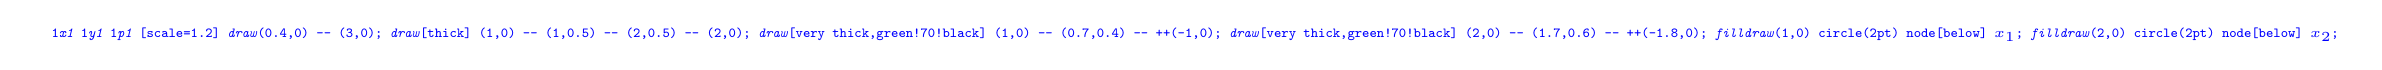
\begin{tikzpicture}[scale=1.2]
	\draw (0.4,0) -- (3,0);

	\draw[thick] (1,0) -- (1,0.5) -- (2,0.5) -- (2,0);

	\draw[very thick,green!70!black] (1,0) -- (0.7,0.4) -- ++(-1,0);
	\draw[very thick,green!70!black] (2,0) -- (1.7,0.6) -- ++(-1.8,0);

	\filldraw (1,0) circle(2pt) node[below] {$x_1$};
	\filldraw (2,0) circle(2pt) node[below] {$x_2$};
	\end{tikzpicture}
	\begin{align*}
		\left\lbrace X \leq x_2 \right\rbrace &=
		\left\lbrace X \leq x_1 \right\rbrace +
		\left\lbrace x_1 < X \leq x_2 \right\rbrace \\
		P\left\lbrace X \leq x_2 \right\rbrace &=
		P\left\lbrace X \leq x_1 \right\rbrace +
		P \left\lbrace x_1 < X \leq x_2 \right\rbrace \\
		\Aboxed{
		F_X(x_2) - F_X(x_1) &= P \left\lbrace x_1<X\leq x_2 \right\rbrace
	}
	\end{align*}

	Ένα αποτέλεσμα του παραπάνω είναι:
	\begin{align*}
	\underset{\epsilon\to 0}{P} \left\lbrace x-\epsilon < X \leq x
	\right\rbrace = F_X(x) - \underset{\epsilon\to 0}{F_X}(x-\epsilon)
	&= F_X(x^+)-F_X(x^-) \\ &= \begin{cases}
	0 & \quad \text{αν είναι συνεχής} \\
	\text{η διαφορά των ορίων} & \quad \text{αν δεν είναι συνεχής}
	\end{cases} \\ &= \mathlarger{P\left\lbrace X=x \right\rbrace}
	\end{align*}

	Παρατηρούμε ότι:
	\begin{align*}
		\text{συνεχής} &\implies P\left\lbrace X=x \right\rbrace = 0\\
		\text{ασυνεχής} &\implies P\left\lbrace X=x \right\rbrace\neq 0
	\end{align*}
	δηλαδή με "πηδήματα" της συνάρτησης κατανομής πιθανότητας, μπορούμε
	να προσδώσουμε πιθανότητα σε σημείο, όπως φαίνεται στα δύο
	παραδείγματα παρακάτω.

	\begin{tikzpicture}[scale=1.2]
	\draw (-4,0) -- (4,0);
	\draw (0,-0.7) -- (0,4) node[left] {$F_X$};
	\draw (0,0) node[below left] {$0$};

	\draw[dashed] (0.7,0) node[below] {$x$} -- (0.7,1) -- (0,1) node[left] {$F_x(x^-)$};
	\draw[dashed] (0.7,2) -- (0,2) node[left] {$F_x(x^+)$};

	\draw[very thick,blue!50!black] plot[smooth] coordinates {(-3,0.5) (-0.2,0.5) (0.7,1)};
	\draw[very thick,blue!50!black] plot[smooth,tension=1] coordinates {(0.7,2) (2.2,3.1) (3.5,3.55)};
	\draw[thick,fill=white] (0.7,1) circle (3pt);
	\draw[thick,fill=black!70!blue] (0.7,2) circle (3pt);

	\begin{scope}[yshift=-4cm]
	\draw (-4,0) -- (4,0);
	\draw (0,-1) -- (0,3) node[below left] {$F_X$};

	\draw[thick,black!70!blue] plot[const plot] coordinates {(-4,0) (.7*1,.7*1) (.7*2,.7*2) (.7*3,.7*3) (.7*4,.7*4) (.7*5,.7*4)};
	\end{scope}
	\end{tikzpicture}

	\subsection{Συνάρτηση Πυκνότητας Πιθανότητας}
	\begin{defn}{Συνάρτηση Πυκνότητας Πιθανότητας}{}
		Ως συνάρτηση πυκνότητας πιθανότητας \( f_X(x) \) ορίζουμε:
		\[
		f_X(x) = \od{F_X(x)}{x}
		\]
	\end{defn}
	\paragraph{Ιδιότητες}
	\begin{enumroman}
		\item \( f_X(x) \geq 0 \)
		\item \( \displaystyle
		\int_{-\infty}^{\infty} f_X(x) \dif x = 1\)
		\item \( \displaystyle
		F_X(x) = \int_{-\infty}^{x} f_X(x)\dif x \)
		\item \( \displaystyle
		P\left\lbrace x_1 < X \leq x_2 \right\rbrace
		= \int_{x_1^+}^{x_2^+} f(x)\dif x \quad
		\mathsmaller{=\ F_X(x_2) - F_X(x_1)}
		\)
	\end{enumroman}

	\begin{center}
	\begin{tikzpicture}[scale=1.6]
	\draw[dashed] (1.8,0) -- ++(0,2.5) (1.8+0.4,0) -- ++(0,2.5);
	\draw[<->] (1.8,2.3) -- ++(0.4,0) node[midway,above,scale=.8] {$\dif x$};
	\begin{scope}
	\clip plot[smooth,tension=.6] coordinates {(-1,0.04) (-0.5,0.3) (1.3,2) (3,0.3) (3.4,0.03)} |- (0,0) -- (-1,0) -- cycle;
	\fill[orange,postaction={pattern=north east lines,opacity=.3},fill opacity=.5] (-1,0) rectangle (0.4,2);
	\fill[orange,postaction={pattern=north east lines,opacity=.3},fill opacity=.5] (1.8,0) rectangle ++(0.4,2);
	\draw (0.4,0) -- ++(0,2);
	\draw (1.8,0) -- ++(0,2) (1.8+0.4,0) -- ++(0,2);
	\end{scope}
	\draw (0.4,0) node[below] {$x_1$};
	\draw (1.8,0) node[below,scale=.7] {$\vphantom{\dif}x$};
	\draw (1.8+0.4,0) node[below,scale=.7] {$x+\dif x$};

	\draw (-1,0) -- (3.5,0);
	\draw (0,-0.2) -- (0,2.5) node[left] {$f_x(x)$};

	\draw[thick,blue!40!black] plot[smooth,tension=.6] coordinates {(-1,0.04) (-0.5,0.3) (1.3,2) (3,0.3) (3.4,0.03)};
	\end{tikzpicture}
	\end{center}

	Παρατηρούμε ότι η συνάρτηση πυκνότητας πιθανότητας μοιάζει π.χ. με
	συνάρτηση πυκνότητας γραμμικής μάζας, και για να λάβουμε την
	πιθανότητα μεταξύ δύο τιμών, απλώς υπολογίζουμε το εμβαδόν της
	συνάρτησης μεταξύ εκείνων των σημείων.

	Μεταξύ των \( f_X(x) \) και \( F_X(x) \) επιλέγουμε αυτήν που μας
	βολεύει περισσότερο, με βάση την ευκολία υπολογισμών. Για
	παράδειγμα, η κανονική κατανομή \( f_X(x) =
	\frac{1}{\sqrt{2\sigma^2\pi} } \; e^{ -\frac{(x-\mu)^2}{2\sigma^2} }
	\) έχει αναλυτική έκφραση, αλλά όχι η αντίστοιχη \( F_X(x) \), για
	την οποία χρειαζόμαστε πίνακες ή υπολογιστή.

	\subsection{Πολλαπλές τυχαίες μεταβλητές}
	Ηχογραφούμε την φωνή μας να λέει την ίδια λέξη κάθε ένα λεπτό. Σε
	κάθε ηχογράφηση παίρνουμε ένα διαφορετικό σήμα:

	\begin{tikzpicture}
	\draw (0,-1) -- (0,2);
	\draw (-1,0) -- (7,0);

	\draw [blue, very thick, name path=a]
	plot [smooth, tension=0.4, domain=0:7, samples=25] (\x,{0.7+rand/1.2});
	\draw [green!50!orange, very thick, name path=b]
	plot [smooth, tension=0.4, domain=0:7, samples=25] (\x,{0.4+rand/1.2});

	\foreach \i in {1,2,...,4} {
		\path[name path=l1] (\i*1.4,-1) -- ++(0,2.5);
		\path[name intersections={of=a and l1,by=m}];
		\path[name intersections={of=b and l1,by=n}];
		\draw[gray!50!black,thick] (m) -- (m |- 0,0)
		node[below,rectangle,align=center,yshift=-4mm] {$t_\i$\\$x(t_\i)$};
		\draw[red!50!black,thick] (n) -- (n |- 0,0);
	}
	\end{tikzpicture}

	Παίρνουμε αυθαίρετα 4 χρονικές στιγμές \( t_1,t_2,t_3,t_4 \). Σε κάθε
	μία από αυτές, η τιμή της έντασης του ήχου για την κάθε ηχογράφηση
	είναι διαφορετική. Για την πρώτη στιγμή, για παράδειγμα, έχουμε μια
	τυχαία μεταβλητή \( X(t_1) \) που εκφράζει την ένταση του ήχου εκείνη
	τη στιγμή, και άλλες 3 αντίστοιχες τυχαίες μεταβλητές για τις \(
	t_2,t_3,t_4 \).

	Τις 4 στιγμές τις επιλέξαμε αυθαίρετα, αλλά το πραγματικό σήμα έχει
	άπειρες τυχαίες μεταβλητές, μία για κάθε στιγμή. Είναι αυτές μεταξύ
	τους ανεξάρτητες;

	\paragraph{Παράδειγμα \#2}
	Έχουμε ένα σύστημα που δέχεται μία μόνο είσοδο \( X \), και παράγει
	μια έξοδο \( Υ \) (που εξαρτάται μόνο από την \( X \)):
	\begin{align*}
		X &= X(J) \\
		Y &= Y(J)
	\end{align*}

	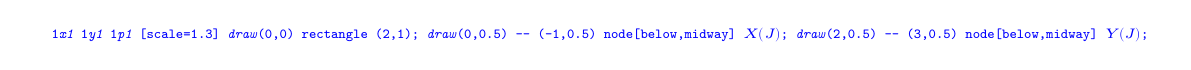
\begin{tikzpicture}[scale=1.3]
	\draw (0,0) rectangle (2,1);
	\draw (0,0.5) -- (-1,0.5) node[below,midway] {$X(J)$};
	\draw (2,0.5) -- (3,0.5) node[below,midway] {$Y(J)$};
	\end{tikzpicture}

	Έστω το ενδεχόμενο \( A \) για το οποίο:
	\[
	A = \left\lbrace X\leq x, Y \leq y \right\rbrace
	= \left\lbrace X \leq x \right\rbrace \cdot
	\left\lbrace Y \leq y \right\rbrace
	\]

	Τότε ορίζουμε μία κοινή πιθανότητα μεταξύ τους (joint probability distribution function):
	\[
	F_X(x,y) = P\left\lbrace X \leq x,\ Y \leq y \right\rbrace
	\]

	\paragraph{Ιδιότητες}
	\begin{enumroman}
		\item \( F(-\infty,y) = F(x,-\infty) = F(-\infty,-\infty)
		= 0 \)
		επειδή:
		\begin{gather*}
			\left\lbrace X=-\infty, Y \leq y \right\rbrace
			\subset \left\lbrace X=-\infty \right\rbrace, \text{ αλλά }
			P\left\lbrace X=-\infty \right\rbrace = 0.
		\end{gather*}

		\item \( F(+\infty,+\infty) = 1 \)
		\item \( F(x,y) \, \uparrow \) αύξουσα ως προς \( x,\ y,\ x \)
		και \( y \) (όχι απαραίτητα γνησίως)

		Για \( x_1<x_2 \), έχουμε:
		\begin{align*}
			P\left\lbrace X\leq x_2,Y\leq y \right\rbrace
			&= P\left\lbrace X\leq x_1, Y \leq y \right\rbrace
			+ P\left\lbrace x_1<X\leq x_2,Y \leq y \right\rbrace\\
			\Aboxed{P\left\lbrace x_1<X\leq x_2,Y\leq y \right\rbrace
			&= F(x_2,y)  - F(x_1,y) \leq 0 \implies F(x_2,y)\geq
			F(x_1,y)}
		\end{align*}

		Με τον παραπάνω τύπο μπορούμε να υπολογίσουμε την πιθανότητα
		μιας κομμένης λωρίδας, όπως φαίνεται στο διάγραμμα:

		\begin{tikzpicture}[scale=1.3]

		\fill[green!50] (0.5,0) rectangle (1.5,1.5);
		\fill[green!50,path fading=south] (0.5,-2) rectangle (1.5,0);

		\draw[->] (-0.5,0) -- (2.5,0) node[below right] {$x$};
		\draw[->] (0,-2) -- (0,2);

		\draw (0.5,0) node[below left] {$x_1$};
		\draw (1.5,0) node[below right] {$x_2$};

		\draw[gray] (0.5,1.5) -- (0.5,2);
		\draw[gray] (1.5,1.5) -- (1.5,2);
		\draw[gray] (0,1.5) -- (2,1.5);

		\draw[thick] (0.5,-2) --
		(0.5,1.5) node[above right,xshift=2mm,rotate=45,scale=.5]{$(x_1,y)$} --
		(1.5,1.5) node[above right,xshift=2mm,rotate=45,scale=.5]{$(x_2,y)$}--
		(1.5,-2);
		\end{tikzpicture}


		\item \( 0 \leq F(x,y) \leq 1 \)
		\item \( F_{XY}(+\infty,y) = F_Y(y) \) \\
		\( F_{XY}(x,+\infty) = F_X(x) \) επειδή
		\begin{align*}
			\left\lbrace X\leq x, Y \leq +\infty \right\rbrace &=
			\left\lbrace X\leq x \right\rbrace\cdot
			\cancelto{S}{\left\lbrace Y \leq +\infty \right\rbrace}
			\\ &\rightarrow P\left\lbrace X\leq x \right\rbrace
		\end{align*}
	\end{enumroman}

	\paragraph{Υπολογισμός πιθανότητας}
	Ποιά είναι η πιθανότητα
	\( \left\lbrace x_1<X\leq x_2,\
	y_1<Y\leq y_2 \right\rbrace \)
	να βρεθούμε μέσα στο ορθογώνιο του σχήματος;

	\begin{tikzpicture}[scale=1.2]
	\fill[green!50!white,path fading=south,opacity=.6] (1,0.4) rectangle (1.5,1);
	\fill[green!50!white] (1,1) rectangle (1.5,1.5);

	\draw[->] (-0.5,0) -- (2,0) node[below right] {$x$};
	\draw[->] (0,-0.5) -- (0,2) node[left] {$y$};

	\draw (1,-0.5) node[above left] {$x_1$} -- (1,2);
	\draw (1.5,-0.5) node[above right] {$x_2$}-- (1.5,2);

	\draw (-0.5,1) node[below] {$y_1$} -- (2,1);
	\draw (-0.5,1.5) node[above] {$y_2$} -- (2,1.5);

	\filldraw[fill opacity=.1] (1,1.5) circle (2.5pt);
	\filldraw[fill opacity=.8] (1.5,1.5) circle (2.5pt);
	\filldraw[fill opacity=.8] (1,1) circle (2.5pt);
	\filldraw[fill opacity=.1] (1.5,1) circle (2.5pt);
	\end{tikzpicture}

	Έχουμε:
	\begin{align*}
	\left\lbrace x_1<X\leq x_2,Y\leq y_2 \right\rbrace
	&= \left\lbrace x_1<X\leq x_2, Y\leq y_1 \right\rbrace
	+ \left\lbrace x_1<X\leq x_2,y_1<Y\leq y_2 \right\rbrace
	\\
	P\left\lbrace x_1<X\leq x_2,Y\leq y_2 \right\rbrace
	&= P\left\lbrace x_1<X\leq x_2, Y\leq y_1 \right\rbrace
	+ P \left\lbrace x_1<X\leq x_2,y_1<Y\leq y_2 \right\rbrace
	\end{align*}
	Άρα:
	\[
	\mathlarger{
		P \left\lbrace x_1<X\leq x_2,\ y_1<Y\leq y_2 \right\rbrace
		= F(x_2,y_2) - F(x_1,y_1) - F(x_2,y_1) + F(x_1,y_1)
	}
	\]
	Δηλαδή μπορούμε να βρούμε την πιθανότητα να "πέσουμε" μέσα στο
	ορθογώνιο (άρα και σε κάθε χωρίο), χρησιμοποιώντας τις
	πιθανότητες από τις άκρες.

	\subsubsection{Συνάρτηση πυκνότητας πιθανότητας (από κοινού)}
	\[
	\mathlarger{f_{XY}(x,y)
			= \frac{\partial^2 F_{XY}(x,y)}{\partial x\,\partial y}
			}
	\]

	\paragraph{Ιδιότητες}
	\begin{enumroman}
		\item \( f(x,y) \geq 0 \)
		\item \( \displaystyle
		\int_{-\infty}^{\infty} \int_{-\infty}^{\infty} f(x,y)\dif x
		\dif y = 1
		 \)
		\item \( \displaystyle
		F(x,y) = \int_{-\infty}^{x}\int_{-\infty}^{y} f(x,y)\dif x\dif y
		 \)
		\item \( \displaystyle
		f_X(x) = \int_{-\infty}^{\infty} f(x,y)\dif y \) \\
		\( \displaystyle
		f_Y(y) = \int_{-\infty}^{\infty} f(x,y)\dif x \)
		\item \( \displaystyle
		P\left\lbrace x_1<X\leq x_2,\ y_1<Y\leq y_2 \right\rbrace
		= \int_{x_1^+}^{x_2^+} \int_{y_1^+}^{y_2^+} f(x,y)\dif x\dif y
		 \)
	\end{enumroman}

	Επομένως για να βρούμε την πιθανότητα ενός χωρίου, αρκεί να
	ολοκληρώσουμε τη συνάρτηση πυκνότητας πιθανότητας σε αυτό.

	\textbf{Παράδειγμα:} Η κανονική κατανομή (καμπάνα)
	για δύο μεταβλητές:

	\begin{tikzpicture}
	\begin{axis}[
	no markers, domain=0:8, samples=50,
	axis lines*=left, xlabel=$x$, ylabel=$y$,
	every axis y label/.style={at=(current axis.above origin),anchor=south},
	every axis x label/.style={at=(current axis.right of origin),anchor=west},
	height=6cm, width=7cm,
	xtick=\empty, ytick=\empty,
	enlargelimits=false, clip=false, axis on top,
	grid = major
	]
	\addplot [very thick,cyan!50!black] {gauss(4,1.5)};
	\end{axis}

	\begin{axis}[xshift=8cm]
	\addplot3[surf,domain=-4:4,domain y=-4:4]
	{exp(-( (x-0)^2 + (y-0)^2)/3 )};
	\node[circle,inner sep=1pt,fill=blue,pin=90:$\mu$]
	at (axis cs:0,0,1) {};
	\end{axis}
	\end{tikzpicture}

	Η κανονική κατανομή δεν μπορεί να ολοκληρωθεί με αναλυτική έκφραση,
	επομένως χρησιμοποιούμε πίνακες ολοκληρωμάτων ή υπολογιστές.

	\paragraph{}
	Τελικά, η συνάρτηση πυκνότητας πιθανότητας είναι μία επιφάνεια,
	η οποία αν ολοκληρωθεί σε κάποιο χωρίο για να λάβουμε τον όγκο που
	καλύπτει, θα πάρουμε την πιθανότητα του χωρίου (μοιάζει με συνάρτηση
	πυκνότητας μάζας).

	\subsection{Συνάρτηση κατανομής υπό συνθήκη πιθανότητας}
	Έστω:
	\[
	A = \left\lbrace X \leq x \right\rbrace
	\qquad
	B = \left\lbrace X \leq x_2 \right\rbrace
	\]

	Τότε:
	\[
	P(A/B) = \frac{P(A\cdot B)}{P(B)}
	\]
	Επομένως μπορούμε να ορίσουμε μια συνάρτηση:
	\[
	\boxed{
		F_X(x/B) = P\left\lbrace X\leq x/B \right\rbrace
		= \frac{P\left\lbrace X\leq x, B \right\rbrace}{P(B)}
		}
	\]
	(όπου το \( P\left\{X\leq x,B\right\}  \) δηλώνει την τομή των
	ενδεχομένων \( X\leq x \) και \(B\))
	για την οποία ισχύουν οι ιδιότητες, αντίστοιχα με προηγουμένως:

	\begin{itemize}
		\item \( F_X(+\infty/B) = 1, \quad F(-\infty/B) = 0 \)
		\item \( \displaystyle
		P\left\lbrace x_1<X\leq x_2\ /B \right\rbrace
		=\frac{P\left\lbrace x_1 < X\leq x_2,\ B \right\rbrace}{P(B)}
		=F(x_2/B) - F(x_1/B) \)
		\item \( \displaystyle f_X(x/B) = \frac{\dif F_X(x/B)}{\dif x} \)
		\item \( f_X(x/B) \leq 0 \ \forall x \)
		\item \( \displaystyle
		\int_{-\infty}^{\infty} f_x(x/B) \dif x = F_X(\infty/B)
		- F_X(-\infty/B) = 1 \)
		\item \( \displaystyle F_X(x_1/B) = \int_{-\infty}^{x_1} f_x(x/B)\dif x \)
		\item \( \displaystyle P \left\lbrace x_1<X\leq x_2\ /B \right\rbrace
		= \int_{x_1^+}^{x_2^+} f_X(x/B)\dif x \)
	\end{itemize}

	Επίσης έχουμε:
	\begin{align*}
		F_X(x/B) &= \begin{cases}
		\frac{F_X(x)}{F_X(x_2)} &\quad x<x_2 \\
		1 &\quad x\geq x_2
		\end{cases} \\
		f_X(x/B) &= \begin{cases}
		\frac{f_X(x)}{\int_{-\infty}^{x^2} f_X(x) \dif x}
		&\quad x<x_2 \\ 0 &\quad x \geq x_2
		\end{cases}
	\end{align*}

	\begin{tikzpicture}[scale=1]
	\draw[->] (-1,0) -- (2.5,0);
	\draw[->] (0,-1) -- (0,2.5);

	\draw[very thick,blue!50!black] plot[smooth] coordinates {(-0.7,0.3) (-0.2,0.2) (1,1.5) (2,1.8)} node[below right] {$F_X(x)$};
	\draw[very thick,green!50!black] plot[smooth] coordinates {(-0.7,0.4) (-0.2,0.6) (0.7,1.6) (1,1.8)} -- (2.5,1.8) node[above] {$F_X(x/B)$};

	\draw[dashed] (1,0) node[below] {$x_2$} -- (1,1.5) -- (0,1.5) node[left] {$F_X(x_2)$};
	\draw[dashed] (1.7,0) node[below] {$x$} -- (1.7,1.8) -- (0,1.8) node[left] {$1$};

	\begin{scope}[yshift=-4cm]
	\draw[->] (-1,0) -- (2.5,0);
	\draw[->] (0,-1) -- (0,2.5);

	\draw[very thick,blue!50!black] plot[smooth] coordinates {(-0.7,0.2) (1,1.5) (2,0.4) (2.5,0.3)} node[above right] {$f_X(x)$};
	\draw[very thick,green!50!black] plot[smooth,tension=1] coordinates {(-0.7,0.5) (0,1.45) (1,2)} -- (1,0) -- (2.4,0) node[below] {$f_X(x/B)$};

	\draw[dashed] (1,0) node[below] {$x_2$} -- (1,1.5);

	\filldraw[green!70!black,opacity=.4] (1,2) circle (2pt);
	\filldraw[green!70!black,opacity=.4] (1,0) circle (2pt);

	\begin{scope}
	\clip (1,0) rectangle (2.5,2);
	\fill[red!70!black,path fading=east] plot[smooth]
	coordinates {(-0.7,0.2) (1,1.5) (2,0.4) (2.5,0.3)} -- (2.5,0) -- (-0.7,0);
	\end{scope}
	\end{scope}
	\end{tikzpicture}

	(θυμόμαστε ότι \(B= \left\{ X\leq x_2 \right\} \))

	\subsubsection{Υπό συνθήκη πιθανότητα με δύο τυχαίες μεταβλητές}

	\paragraph{Έστω} ότι \( A=\left\lbrace X \leq x \right\rbrace
	\qquad B = \left\lbrace Y \leq y \right\rbrace
	\)
	\[
	\boxed{F_X(x/B)
		= \frac{F_{XY}(x,y)}{F_Y(y)}}
	\]

	Για τη συνάρτηση πυκνότητας πιθανότητας:
	\begin{align*}
		\pd{F_{XY}(x,y)}{x} &= \pd{}{x} \left[
		\int_{-\infty}^{y} \int_{-\infty}^{x} f_{XY} (x,y)\dif x\dif y
		\right] \\ &=
		\int_{-\infty}^{y} \left[\pd{}{x}\int_{-\infty}^{x}f(x,y)
		\dif x\right]\dif y = \int_{-\infty}^{y} f_{XY}(x,y)\dif y
	\end{align*}

	Άρα:
	\begin{align*}
		f_X (x,\ Y \leq y) &= \frac{1}{F_Y(y)}\pd{F_{XY}(x,y)}{x} \\
		&= \frac{\int_{-\infty}^{y}f_{XY}(x,y)\dif y}{
			\int_{-\infty}^{\infty} \int_{-\infty}^{y}
			f(x,y)\dif y\dif x}
	\end{align*}

    \paragraph{Έστω όμως} ότι
    \( B = \left\lbrace y_1 < Y \leq y_2 \right\rbrace \)

    \begin{align*}
    	F_X(x/\ y_1 < Y \leq y_2) &=
    	\frac{P\left\lbrace x\leq x,\ y_1 < Y \leq y_2\right\rbrace}{
    		P\left\lbrace y_1 < Y \leq y_2 \right\rbrace}
    	\\ &= \frac{F_{XY}(x,y_2) - F_{XY}(x,y_2)}{
    		F_Y(y_2)-F_Y(y_1)}
    	\\ &= \frac{\int_{y_1}^{y_2} f_{XY}(x,y)\dif y}{
    		\int_{-\infty}^{\infty} \int_{y_1}^{y_2} f_{XY}(x,y)
    		\dif y\dif x}
    \end{align*}

    \todo{fix}
    \paragraph{Έστω ότι \( B = \left\lbrace Y=y \right\rbrace \)}
    \begin{align*}
    	F_X(Y=y) &= \frac{
    		\sfrac{\partial F_{XY}(x,y)}{\partial\. y} }{
    		\sfrac{\dif }{den} }\quad????
    \end{align*}

    \subsection{Ανεξαρτησία Τυχαίων Μεταβλητών}
    Ο γνωστός ορισμός της ανεξαρτησίας είναι:
    \[
    P(A\cdot B) = P(A) \cdot P(B)
    \]

    Επομένως, για δύο τυχαίες μεταβλητές \( X,Y \) και τα αντίστοιχα
    ενδεχόμενα \( A=\left\lbrace X\leq x \right\rbrace \) και
    \( B = \left\lbrace Y \leq y \right\rbrace \), έχουμε:
    \begin{align*}
    	P\left\lbrace X\leq x,\ Y\leq y \right\rbrace &=
    	P\left\lbrace X \leq x \right\rbrace \cdot
    	P\left\lbrace Y \leq y \right\rbrace \\
    	F_{XY}(x,y) &= F_X(x) \cdot F_Y(y) \\
    	\xRightarrow{\frac{\partial^2 F(x,y)}{\partial x\,\partial y}}
    	f_{XY}(x,y) &= f_X(x)\cdot f_Y(y)
    \end{align*}

    Άρα για δύο ανεξάρτητες τυχαίες μεταβλητές ισχύει:
    \begin{align*}
    	F_X(x/\ Y\leq y) = \frac{P\left\lbrace X\leq x,\ Y\leq y
    		 \right\rbrace}{P\left\lbrace Y\leq y \right\rbrace}
        = P\left\lbrace X\leq x \right\rbrace = F_X(x)
    \end{align*}

    \subsection{Ντετερμινιστική σχέση μεταξύ τυχαίων ματαβλητών}
    \[ \mathlarger{\left(X,f_X(x)\right)
    \xrightarrow{\qquad} \left(Y,f_Y(y)\right)}
    \]

    Έστω ότι υπάρχει μία \textit{ντετερμινιστική} σχέση \( g(\cdot) \)
    που συνδέει τις
    \textit{τυχαίες} μεταβλητές \( X,Y \):
    \[
    \mathlarger{Y=g(X)}
    \]

    Ομοίως μπορεί να έχουμε:
    \(
    (X,Y,f_{XY}(x,y)) \to (Z,W,f_{ZW}(z,w))
     \)

    \( Z =g(X,Y)\)

    \( W=h(X,Y) \)

	\todo{add more text}
	\begin{tikzpicture}[scale=1.1]
	\begin{scope}
	\clip plot[smooth] coordinates {(-0.7,0.2) (1,1.5) (3,0.4) (3.7,0.2)} -- (3.7,0) -- (-0.7,0);
	\fill[orange,postaction={pattern=north east lines,opacity=.3},fill opacity=.5] (1,0) rectangle ++(0.4,2);
	\draw[dashed] (1,0) -- ++(0,2) (1+0.4,0) -- ++(0,2);
	\end{scope}

	\draw[->] (-1,0) -- (2.5,0) node[below right] {$x$};
	\draw[->] (0,-1) -- (0,2.5);

	\draw[thick,blue!40!black] plot[smooth] coordinates {(-0.7,0.2) (1,1.5) (3,0.4) (3.7,0.2)} node[right] {$f_X$};
	\draw[dashed] (1,1.5) -- (0,1.5) node[left] {$f_X(x)$};

	\draw (current bounding box.south) node[below,align=center] {
		$f_X(x_0)\dif x = P\big\{ x_0<x<x_0+\dif x\big\}$ \\
		$f_Y(y)\dif x = P\big\{ y<Y<y+\dif y\big\}$
	};
	\draw (current bounding box.south east) node[above right,scale=.7] {$\big(y=g(x)\big)$};
	\end{tikzpicture}

	\begin{tikzpicture}[scale=1.7,xscale=1.5]
	\begin{scope}
	\clip plot[smooth] coordinates {(-1.5,0.4) (-0.3,2) (1.2,1) (1.6,2) (2.2,1.6) (3,3)} -- (3,-1) -- (-1.5,-1);
	\fill[cyan,postaction={pattern=north east lines,opacity=.3},fill opacity=.5]
	(-0.65,0) rectangle ++(0.4,3)
	(1.64,0) rectangle ++(0.32,3)
	(2.3,0) rectangle ++(0.2,3)
	;
	\draw[dashed,every node/.style={scale=.5}]
	(-0.65,0) node[below] {$x_1+\dif x_1$} -- ++(0,3)
	(-0.65+0.4,0) node[below] {$\vphantom{\dif}x_1$} -- ++(0,3)
	(1.64,0) node[below] {$\vphantom{\dif}x_2$} -- ++(0,3)
	(1.64+0.32,0) node[below] {$x_2+\dif x_2$} -- ++(0,3)
	(2.3,0) node[below] {$x_3+\dif x_3$} -- ++(0,3)
	(2.3+0.2,0) node[below] {$\vphantom{\dif}x_3$} -- ++(0,3)
	;
	\end{scope}

	\draw[->] (-2,0) -- (3,0) node[below right] {$x$};
	\draw[->] (0,-1) -- (0,2.5) node[left] {$y$};

	\draw[thick,blue!40!black] plot[smooth] coordinates {(-1.5,0.4) (-0.3,2) (1.2,1) (1.6,2) (2.2,1.6) (3,3)} node[above] {$y=g(x)$};

	\draw[dashed] (-0.2,2) -- (2.5,2);
	\draw[dashed] (-0.65,1.7) -- (2.3,1.7);

	\filldraw[green!50!cyan!90!black,thin,fill opacity=.4]
	(-0.65,1.7) circle (1pt)
	(-0.65+0.4,2) circle (1pt)
	(1.64,2) circle (1pt)
	(1.64+0.32,1.7) circle (1pt)
	(2.3,1.7) circle (1pt)
	(2.3+0.2,2) circle (1pt)
	;
	\end{tikzpicture}

	\begin{align*}
	f_Y(y)\dif y &= P\left\lbrace y<Y\leq y+\dif y \right\rbrace \\
	&= P\left\lbrace x_1<X\leq x_1+\dif x_1 \right\rbrace
	+ P\left\lbrace x_2<X\leq x_2+\dif x_2 \right\rbrace
	+ P\left\lbrace x_3<X\leq x_3+\dif x_3 \right\rbrace
	\end{align*}

	Άρα:
	\begin{align*}
		f_Y(y) &=  f_X(x_1) \frac{|\dif x_1|}{\dif y}
		+ f_X(x_2)\frac{|\dif x_2|}{\dif y}
		+ f_X(x_3)\frac{|\dif x_3|}{\dif y} \\
		\Aboxed{ f_Y(y) &= \frac{f_X(x_1)}{\left|g'(x_1)\right|}
		+ \frac{f_X(x_2)}{\left|g'(x_2)\right|}
		+ \frac{f_X(x_3)}{\left|g'(x_3)\right|}}
	\intertext{και γενικότερα}
	    \Aboxed{
	    	f_Y(y) &= \sum_{i=1}^{m} \left.
	    	 \frac{f_X(x)}{\left|g'(x)\right|}
	    	\right|_{x=x_i}
	    	}
	\end{align*}

	\paragraph{Για δύο ζευγάρια τυχαίων μεταβλητών}
	προκύπτει ότι, για \( z=g(x_i,y_i) \) και \( w=h(x_i,y_i) \):
	\[
	\boxed{
		f_{ZW}(z,w) = \sum_{i=1}^{n} \left.
		\frac{f_{XY}(x,y)}{\left|\mathrm J(x,y)\right|}
		\right|_{\scriptsize \begin{matrix}
			x=x_i \\ y=y_i
			\end{matrix}}
		}
	\]

	όπου \( \mathrm J \) η ιακωβιανή ορίζουσα \(
	\mathrm J = \left|\begin{matrix}
	\pd{g(x,y)}{x} & \pd{g(x,y)}{y} \\
	\pd{h(x,y)}{x} & \pd{h(x,y)}{y}
	\end{matrix}\right|.
	 \)

	\paragraph{Παράδειγμα}
	Έστω ότι έχουμε ένα μοντέλο \( \left(X,Y,f_{XY}\right) \), και τις
	τυχαίες μεταβλητές:
	\begin{align*}
		Z &= g(X,Y) \leftrightarrow f_Z(z) \\
		W &= X = h(X,Y)
	\end{align*}

	Τότε έχουμε:
	\begin{align*}
	    f_Z(z) &= \int_{-\infty}^{\infty} f_{ZW}(z,w)\dif w\\
		f_{ZW}(z,w) &= \sum_{i=1}^{n} \left.
		\frac{f_{XY}(x,y)}{\left|J(x,y)\right|} \right|_{x=x_i,\ y=y_i}
	\end{align*}

	\paragraph{Παράδειγμα}
	Έστω μοντέλο \( \left(X,Y,f_{XY}\right) \) και οι:
	\begin{align*}
		Z &= X+Y \\
		W &= X
	\end{align*}

	Αν λύσουμε το παραπάνω σύστημα, έχουμε:
	\begin{align*}
		y_1 &= z-w \\
		x_1 &= w
	\end{align*}

	Επομένως:
	\begin{align*}
		J(x) &= \left|\begin{matrix}
		1 & 1 \\ 1 & 0
		\end{matrix}\right| = -1\\
		f_{ZW}(z,w) &= \left. \frac{f_{XY}(x,y)}{|-1|}
		\right|_{x_1=w,\ y_1=z-w} \\ &= f_{XY}(w,\ z-w)
	\end{align*}

	Έχει ενδιαφέρον όταν οι \( X \) και \( Y \) είναι ανεξάρτητες,
	οπότε:
	\begin{align*}
		f_{XY}(x,y) &= f_X(x) \cdot f_Y(y) \\
		f_{ZW}(z,w) &= \left. \frac{f_X(x)f_Y(y)}{|-1|}\right|_{
			x_1=w,\ y_1=z-w} \\
		f_Z(z) &= \int_{-\infty}^{\infty} f_X(w)f_Y(z-w)
		= f_X(z)
\underset{\substack{\downarrow\\\mathclap{\text{συνέλιξη}}}}{*}
		 f_Y(z)
	\end{align*}

\subsection{Χρήση γενικευμένων συναρτήσεων}
Οι συναρτήσης κατανομής και πυκνότητας πιθανότητας που
χρησιμοποιούμε μπορεί να μην είναι συνεχείς ή παραγωγίσιμες:
\begin{tikzpicture}[scale=1.2,xscale=1.1]
\draw[->] (-1,0) -- (4,0);
\draw[->] (0,-1) -- (0,4) node[left] {$F_X(x)$};

\draw[very thick,black!60!blue] plot[const plot] coordinates
{(-1,0) (.7*1,.3+.7*1) (.7*2,.3+.7*2) (.7*3,.3+.7*3) (.7*4,.3+.7*4) (.7*5,.3+.7*4)};

\def\x{1}
\draw (0.7*\x,0) node[below] {$x_1$};
\draw[fill=white] (0.7*\x,{1*(\x-1)}) circle (2pt);
\draw[fill=black!70!blue] (0.7*\x,{1*(\x)}) circle (2pt);
\foreach \x in {2,3,4} {
	\draw[dashed] (0.7*\x,0) node[below] {$x_\x$} -- (0.7*\x,{.3+0.7*(\x-1)});
	\draw[fill=white] (0.7*\x,{.3+0.7*(\x-1)}) circle (2pt);
	\draw[fill=black!70!blue] (0.7*\x,{.3+0.7*(\x)}) circle (2pt);
}

\draw[dashed] (2.8,3.1) -- (0,3.1) node[left] {$1$};

\begin{scope}[yshift=-3.5cm]
\draw[->] (-1,0) -- (4,0);
\draw[->] (0,-1) -- (0,2) node[left] {$f_X(x)$};

\draw[very thick,black!60!blue] plot[const plot] coordinates {(-1,0) (3.7,0)};
\def\x{1}
\draw[very thick,black!50!blue,->] (0.7*\x,0) node[below,black] {$x_\x$} -- ++(0,1) node[above] {$P_\x$};
\foreach \x in {2,3,4} {
	\draw[very thick,black!50!blue,->] (0.7*\x,0) node[below,black] {$x_\x$} -- ++(0,.7) node[above] {$P_\x$};
}
\end{scope}
\end{tikzpicture}

\begin{align*}
	P(X=x_i) &= p_i = F_X(x_i) - F_X(x_i^-) \\
	\sum_i p_i &= \cancelto{1}{F_X(+\infty)} -
	 \cancelto{0}{F_X(-\infty)} = 1 \\
	F_X(x) &= \sum_i P \left\lbrace X=X_i \right\rbrace
\end{align*}

Απ' ό,τι βλέπουμε, η συνάρτηση πυκνότητας πιθανότητας στο
παραπάνω σχήμα δεν είναι πεπερασμένη, αλλά περιέχει τέσσερις
\textbf{ώσεις}, δηλαδή συναρτήσεις \( \delta(t) \):
\[
f_X(x) = \sum_i p_i \delta(x-x_i)
\]

Αυτή ήταν μία συνάρτηση που περιείχε μόνο ώσεις. Αντίστοιχα,
μπορούμε να έχουμε μικτές συναρτήσεις:

\begin{tikzpicture}[scale=1.5]
\draw[->] (-1,0) -- (4,0);
\draw[->] (0,-1) -- (0,4) node[left] {$F_X(x)$};


\draw[dashed] (1,1) --  (1,0) node[below] {$x_1$};
\draw[dashed] (1.5,2.55) --  (1.5,0) node[below] {$x_2$};


\draw[very thick,blue!50!black] plot[smooth] coordinates {(-1,0.4) (-0.2,0.5) (1,1)};
\draw[very thick,blue!50!black] plot[smooth,tension=1] coordinates {(1,2) (1.2,2.3) (1.5,2.55)};
\draw[very thick,blue!50!black] plot[smooth,tension=1] coordinates {(1.5,3) (2.3,3.4) (3.7,3.53)};
\draw[blue!50!black] (1,1) -- (1,2) (1.5,2.55) -- (1.5,3);
\draw[thick,fill=white] (1,1) circle (2pt);
\draw[thick,fill=black!70!blue] (1,2) circle (2pt);
\draw[thick,fill=white] (1.5,2.55) circle (2pt);
\draw[thick,fill=black!70!blue] (1.5,3) circle (2pt);


\draw[dashed] (3.7,3.6) -- (0,3.6) node[left] {$1$};

\begin{scope}[yshift=-3.5cm]
\draw[->] (-1,0) -- (4,0);
\draw[->] (0,-1) -- (0,2) node[left] {$f_X(x)$};

\draw[very thick,black!60!blue,->] (1,0) -- ++(0,0.7);
\draw[very thick,black!60!blue,->] (1.5,0) -- ++(0,0.7);

\draw[very thick,black!60!blue,mark position=0.5(a),mark position={(1+1)/(1+4)}(b)]
plot[smooth,tension=.6] coordinates {(-1,0.04) (-0.5,0.3) (1.4,2) (3,0.3) (3.7,0.03)};

\draw[dashed] (1,1.84) --  (1,0) node[below] {$x_1$};
\draw[dashed] (1.5,2.00) --  (1.5,0) node[below] {$x_2$};
\draw[thick,fill=white] (1,1.84) circle (2.5pt);
\draw[thick,fill=white] (1.5,2.00) circle (2.5pt);
\end{scope}
\end{tikzpicture}

\section{Ροπές}
Έχουμε το μοντέλο:
\[
\left(\mathlarger{\mathlarger{X,f_X(x)}}\right)
\]

Αν γνωρίζουμε την \( f_X(x) \), μπορούμε να κάνουμε όποιον
υπολογισμό θέλουμε για την τυχαία μεταβλητή, αλλά συχνά είναι
πολύ δύσκολο να βρούμε τη συνάρτηση αυτή. Τότε χρησιμοποιούμε
προσεγγίσεις που προκύπτουν από τις ροπές, που θα δούμε παρακάτω.

Οι ροπές είναι μεγέθη (μέσος όρος, τυπική απόκλιση κλπ.) που
προκύπτουν από στατιστικά δεδομένα.

\subsection{Χαρακτηριστική συνάρτηση}
\begin{defn}{Χαρακτηριστική συνάρτηση τυχαία μεταβλητής}{}
	\[
	\Phi(\omega ) = \int_{-\infty}^{\infty} f_X(x) e^{j\omega x}
	\dif x
	\]
\end{defn}
Παρατηρούμε ότι ουσιαστικά είναι ένας αντίστροφος μετασχηματισμός
Fourier, και ότι η αντίστροφη διαδικασία είναι:
\[
f_X(x) = \frac{1}{2\pi} \int_{-\infty}^{\infty}
\underline{\Phi(\omega )} e^{-j\omega x}\dif \omega
\]

\paragraph{Ιδιότητες}
\begin{enumpar}
	\item \( \displaystyle \Phi(0)
	= \int_{-\infty}^{\infty} f(x)\dif x = 1 \)
	\item \( \displaystyle \left| \Phi(\omega ) \right| = \left|
	\int_{-\infty}^{\infty} e^{-j\omega x}\dif x
	\right|
	\leq \left|\int_{-\infty}^{\infty} f(x)\dif x\right| = 1
	\implies \boxed{\left|\Phi(\omega )\right|\leq1}
	\)

	Γενικά, αν \( \omega \neq 0 \), τότε \( \left|
	\Phi(\omega ) < 1
	\right| \) (με μία εξαίρεση)
	\item \( F_X(x) \leftarrow \Phi(\omega ) \):

	\begin{align*}
		P\left\lbrace x_1 < x \leq x_2 \right\rbrace
		&= \boxed{F_X(x_2) - F_X(x_1)}
		\\ &= \int_{x_1}^{x_2} f_X(x)\dif x
		\\ &= \frac{1}{2\pi} \int_{x_1}^{x_2}
		\int_{-\infty}^{\infty} \Phi(\omega )e^{-j\omega x}
		\dif \omega \dif x = \boxed{
			\frac{1}{2\pi} \int_{-\infty}^{\infty}
			\Phi(\omega) \cdot
			\frac{e^{-j\omega x_2}-e^{-j\omega x_1}}{-j\omega }
			\dif \omega
			}
	\end{align*}
\end{enumpar}

Μέχρι στιγμής έχουμε μια συνάρτηση που μπορεί να μας οδηγήσει στην
\( f_X(x) \). Πώς μπορούμε να την βρούμε;

\begin{align*}
	e^{j\omega x} &= \sum_{k=-\infty}^{\infty}
	\frac{(j\omega x)^k}{k!} \\
	\Phi(\omega ) &= \int_{-\infty}^{\infty} f_X(x)
	\sum_{k=0}^{\infty} \frac{(j\omega x)^k}{k!}\dif x
	= \sum_{k=0}^{\infty} \frac{(j\omega x)^k}{k!}
	f_X(x)\dif x
	\\ &= \sum_{k=0}^{\infty} \frac{(j\omega )^k}{k!}
	\left[
	\int_{-\infty}^{k} x^k f_X(x)\dif x
	\right]
\end{align*}


\subsubsection{Ορισμός}
\begin{defn}{Ροπή}{}
	Ονομάζουμε \( \mathbf{k} \)\textbf{-οστή ροπή} τον αριθμό:
	\[
	\mathlarger{m_k
	= \int_{-\infty}^{\infty} x^K f_X(x)\dif x
	}
	\]
\end{defn}

Τότε:
\[
\boxed{\mathlarger{
		\Phi(\omega ) = \sum_{k=0}^{\infty}
		\frac{(j\omega )^k}{k!} \cdot m_k
		}}
\]

Παρατηρούμε ότι η ροπή με \( k=1 \) είναι η \textit{μέση τιμή} μιας
μεταβλητής. Επίσης παρατηρούμε ότι για να βρούμε τις συναρτήσεις
πυκνότητας \& κατανομής πιθανότητας, χρειαζόματε τον άπειρο
αριθμό ροπών, αλλά με μεγάλο \( k \), αυξάνεται ο παρονομαστής,
και μετράν όλο και λιγότερο στο τελικό αποτέλεσμα.

Δηλαδή:
\begin{align*}
\Phi(\omega ) &= 1 + j\omega m_1
+ \frac{(j\omega )^2}{2!}m_2 + \dots +
\frac{(j\omega )^k}{k!}m_k + \dots \\
\od{\Phi(\omega )}{\omega } &= jm_1 + \frac{2(j\omega )j}{2!}m_2
+ \dots + \frac{k(j\omega )^{k-1}j^k}{k!}m_k + \dots\\
\left.\od{\Phi(\omega )}{\omega }\right|_{\omega =0}&=jm_1
\intertext{Και γενικότερα:}
\left.\Phi^{(k)}(\omega )\right|_{\omega = 0} &= j^k m_k
\end{align*}

Δηλαδή μπορούμε από την \( k \)-οστή παράγωγο της χαρακτηριστικής
συνάρτησης στο \( \omega = 0 \) να βρούμε την \( k \)-οστή ροπή.

\subsection{Μέση τιμή}
\subsubsection{Σε μία μεταβλητή}

\paragraph{Διακριτή \( f_X \)}
Έστω ότι η \( f_X \) είναι διακριτή, δηλαδή προκύπτει από ώσεις.
\[
m_1 = \int_{-\infty}^{\infty} xf-X(x)\dif x
\]

Την πρώτη ροπή ονομάζουμε μέσο όρο:
\[
m_1 = E[x] = \sum_{i} x_i f_X(x_i)
\]

\paragraph{Παράδειγμα - ηλικίες}
\begin{tabular}{cccc}
	Πατέρας & Μητέρα & Παιδί 1 & Παιδί 2 \\
	40 & 28 & 5 & 3 \\
	\end{tabular}
\begin{align*}
\text{Μ.Ο } &= \frac{40+28+5+3}{4} = 19
\\ &= \frac{1}{4}40 + \frac{1}{4}28 + \frac{1}{4}5
+ \frac{1}{4}3
\end{align*}

Όμως δεν υπάρχει στην οικογένεια άτομο με ηλικία (κοντά στα) 19 έτη!

Αν παρομοιάσουμε το παραπάνω με ένα πείραμα τύχης με δειγματικό
χώρο:
\[
S = \left\lbrace \varPi, M, \varPi_1, \varPi_2 \right\rbrace
\]
όπου η τυχαία μεταβλητή \( x \) είναι η ηλικία και έχουμε ίδια
πιθανότητα \( f(x_i) = \frac{1}{4} \) να επιλέξουμε ένα άτομο,
έχουμε:
\[
E[x] = \sum_{i=1}^{4} x_if_X(x) = \frac{1}{4}40 + \frac{1}{4}28 + \frac{1}{4}5 + \frac{1}{4}3
\]
\paragraph{Μία ενδιαφέρουσα ιδιότητα}\hspace{0pt}\par
\begin{tikzpicture}
\draw[draw=blue!50!green,fill=green,fill opacity=.5,postaction={pattern=north east lines,opacity=.2}] (-0.2,0) rectangle (2.3,0.797115095315);

\begin{scope}[]
\clip plot [variable=\x,domain=-0.3:2.5,samples=40,yscale=.5]
(\x,-3.47852*\x^6+19.8404*\x^5-33.1088*\x^4+1.97819*\x^3+36.2435*\x^2-21.1624*\x+1)
-- (2.5,0) -- (-0.3,0);
\fill[yellow!90!brown,opacity=.7,postaction={pattern=north west lines,opacity=.2}]
(-0.2,2) rectangle (2.3,-2);
\draw[dashed] (-0.2,0) -- ++(0,2);
\draw[dashed] (2.3,0) -- ++(0,2);
\end{scope}

\draw[blue,very thick] plot [variable=\x,domain=-0.3:2.5,samples=150,yscale=.5]
(\x,-3.47852*\x^6+19.8404*\x^5-33.1088*\x^4+1.97819*\x^3+36.2435*\x^2-21.1624*\x+1);

\draw (-1,0) -- (3,0);
\draw (0,-1.5) -- (0,2);
\end{tikzpicture}

Το εμβαδόν μιας συνάρτησης σε ένα διάστημα είναι ίσο με το ορθογώνιο
που έχει ύψος τη μέση τιμή της συνάρτησης στο διάστημα αυτό.

\subsubsection{Σε πολλές μεταβλητές}
Αν μία τυχαία μεταβλητή \( Y \) εξαρτάται από την \( X \):
\[
Y = g(X)
\]
τότε προκύπτει:
\begin{align*}
E[y] &= \int_{-\infty}^{\infty} yf_Y(y)\dif y \\
E[y] &= \bar y = \int_{-\infty}^{\infty} g(X)\dif x
\end{align*}
δηλαδή προκύπτει με απλή ολοκλήρωση της \( g \).

\subsubsection{Ιδιότητες}
\begin{enumparen}
	\item \( E[C] = C \)
	\item \( E[Cx] = CE[x] \)
	\item \( E\left[g_1(x)+g_2(x)+\dots+g_n(x)\right]
	= E\left[g_1(x)\right] + E\left[g_2(x)\right] + \dots
	+ E\left[g_n(x)\right]
	\)
\end{enumparen}

\subsection{Δεύτερη ροπή}
\begin{align*}
	m_2 &= \int_{-\infty}^{\infty} x^2 f_X(x) \dif x\\
	m_2 &= E[x^2] = \overline{x^2}
\end{align*}

Αν η τυχαία μεταβλητή μας είναι το ρεύμα ή η ένταση, η ροπή αυτή
μπορεί να αναπαριστά ισχύ (επειδή υψώνεται η τυχαία μεταβλητή
στο τετράγωνο).

\subsection{Κεντρική ροπή}
\begin{defn}{Κεντρική ροπή}{}
	\begin{align*}
	\mathlarger{\mu_k}
	 = \int_{-\infty}^{\infty} (x-\bar x)^k f_X(x)\dif x
	\end{align*}
	\( y=(x-\bar x)^k \)
\end{defn}
(οι προηγούμενες ροπές που μελετήσαμε λέγονταν κανονικές)

\begin{tikzpicture}
\begin{axis}[
no markers, domain=-4:4, samples=100,
axis y line=center,
axis x line=middle,
ylabel=$f_x(x)$,
height=6cm, width=7cm,
xtick=\empty, ytick=\empty,
enlargelimits=false, clip=false, axis on top,
enlarge y limits=0.15,
grid = major
]
\addplot [very thick,cyan!50!black] {gauss(0,1.5)};
\draw[<->] (0,0.07) -- (1.5,0.07) node[midway,above] {$x-\bar x$};
\draw[dashed] (1.5,0) -- (1.5,0.16);
\draw (0,0) node[below left] {$\bar x$};
\end{axis}
\end{tikzpicture}

Παρατηρούμε ότι:
\[
E\left[(x-\bar x)^k\right] = \mu_k
\]

Αν έχουμε ένα "τραίνο ώσεων", δηλαδή η τυχαία μεταβλητή μας είναι
διακριτή (ή θεωρήσουμε πως είναι διακριτή):
\begin{align*}
	\mu_k &= \sum_i (x_i-\bar x)^k f_X(x_i) \\
	\mu_k &= E\left[(x-\bar x)^k\right]
	= E\left[\sum_{\tau = 0}^{k}
	\binom{k}{\tau} (-1)^\tau (\bar x)^\tau x^{k-\tau}
	\right] = \sum_{\tau = 0}^{k} \binom{k}{\tau}
	(-1)^\tau (\bar x)^\tau \cancelto{m_{k-\tau}}{E[x^{k-\tau}]}
\end{align*}


\subsubsection{Τυπική απόκλιση}
Η τυπική απόκλιση προκύπτει από την κεντρική ροπή με \(k=2\):
\begin{align*}
	\mu_2 &= \int_{-\infty}^{\infty} (x-\bar x)^2 f_X(x)\dif x \\
	&= \int x^2 f(x)\dif x - 2 \bar x^2 \int x f(x) \dif x +
	(\bar x)^2 \cancelto{1}{\int f(x) \dif x} \intertext{Δηλαδή:}
	\mu_2 &= m_2 - \bar x^2 \\
	\mu_2 &= m_2 - (m_1)^2 \\
	\sigma_x^2 &= E[x^2] - \left(E[x]\right)^2
\end{align*}
όπου ονομάζουμε το \( \sigma^2 \) \textbf{διασπορά} και την
\( \sqrt{\sigma^2} \) \textbf{τυπική απόκλιση}, και εκφράζουν το πόσο
μεγάλο "εύρος" καταλαμβάνει η κατανομή στη συνάρτηση πυκνότητας
πιθανότητας.

\subsection{Για δύο τυχαίες μεταβλητές}
\begin{defn}{Ροπή \( kr \)}{}
	Έστω \[
	(X,Y,f_{XY}(x,y))
	\]
	\tcblower
	Ορίζουμε \textbf{ροπή} \( \mathbf{kr} \) τον αριθμό:
	\[
	m_{kr} = \int_{-\infty}^{\infty} \int_{-\infty}^{\infty}
	x^k y^r f_{XY}(x,y)\dif x\dif y \ = E[x^ky^r]
	\]
	και λέμε \( n = k+r \).
\end{defn}
\begin{defn}{Κεντρική Ροπή \( kr \)}{}
	\textbf{Κεντρική ροπή} είναι:
	\[
	\mu_{kr} = \int_{-\infty}^{\infty} \int_{-\infty}^{\infty}
	(x-\bar x)^k (y-\bar y)^r f_{XY}(x,y)\dif x\dif y
	 = E \left[(x-\bar x)^k(y-\bar y)^r\right]
	\]
\end{defn}

Για \( m_{11} \), ορίζουμε συγκεκριμένα την \textbf{συσχέτιση}:
\begin{defn}{Συσχέτιση}{}
	\[
	m_{11} = E[XY] = \int_{-\infty}^{\infty} \int_{-\infty}^{\infty}
	xy f(x,y)\dif x \dif y
	\]
\end{defn}

Αντίστοιχα, την \textbf{συμμεταβλητότητα} (covariance –
\( \cov \)):
\begin{defn}{Συμμεταβλητότητα}{}
	\[
	\mu_{11} = E\left[
	(x-\bar x)(y-\bar y)
	\right]
	\]
\end{defn}

Αν κάνουμε μερικές πράξεις:
\begin{align*}
	\mu_{11} &= E\left[(x-\bar x)(y-\bar y)\right] \\
	&= E[xy-\bar x y-\bar y x +\bar x\bar y] \\
	&= E[xy]-\bar xE[y]-\bar y E[x] +\bar x \bar y \\
	&= E[xy] - E[x]E[y] \\
	&= m_{11} - E[x]E[y]
\end{align*}

Τους παραπάνω ορισμούς θα τους χρησιμοποιήσουμε για να ορίσουμε τον
\textit{συντελεστή συσχέτισης}.

Στο αναλογικό σήμα υπάρχει η χρονική συσχέτιση, που ορίζεται ως εξής:
\[
\lim_{T\to \infty} \frac{1}{T} \int_{-\sfrac{T}{2} }^{\sfrac{T}{2} }
x(t)y(t)\dif t
\]

Εδώ, η συσχέτιση δείχνει ότι υπάρχει κάποια στατιστική
σχέση/αλληλοεξάρτηση μεταξύ δύο μεταβλητών. Η συμμεταβλητότητα είναι
η συσχέτιση, μειωμένη κατά έναν σταθερό όρο. Αν η μέση τιμή κάποιας
από τις δύο μεταβλητές είναι 0, τότε η συμμεταβλητότητα ισούται με τη
συσχέτιση.

\subsubsection{Συντελεστής Συσχέτισης}

Πριν ορίσουμε το συντελεστή συσχέτισης, θα \textbf{κανονικοποιήσουμε}
τις μεταβλητές μας, ώστε να αναφερόμαστε σε όμοια μεγέθη:
\[
z=\frac{x-\bar x}{\sigma_x}
\qquad \theta = \frac{y-\bar y}{\sigma_y}
\]

Παρατηρούμε ότι έχουν μέση τιμή \( \bar z=\bar \theta \):
\[
\bar z = E[z]=E\left[\frac{x-\bar x}{\sigma_x}\right]
= \frac{1}{\sigma_x}\cancelto{0}{\left(E[x]-\bar E[x]\right)} = 0
\]
Δηλαδή η κανονικοποίηση μετακίνησε τη μέση τιμή των μεταβλητών στο 0.

Για τη μεταβλητότητα έχουμε:
\begin{align*}
\sigma_z^2 &= E\left[(z-\cancelto{0}{\bar z})\right]
\\ &= E[z^2] = E\left[\left(\frac{x-\bar x}{\sigma^2}\right)\right]
= 1
\end{align*}

Δηλαδή:
\begin{align*}
\bar z = \bar \theta &= 0 \\
\sigma_z^2 = \sigma_\theta^2 &= 1
\end{align*}

Ορίζουμε τον \textbf{συντελεστή συσχέτισης} \( \rho \) ως την αναμενόμενη
τιμή ενός γινομένου:
\begin{defn}{Συντελεστής Συσχέτισης}{}
	\begin{align*}
	\rho &= E\left[\left(
	\frac{x-\bar x}{\sigma_x}
	\right)\left(
	\frac{y-\bar y}{\sigma_y}
	\right)
	\right] \\ &= \int_{-\infty}^{\infty} \int_{-\infty}^{\infty}
	\frac{(x-\bar x)(y-\bar y)}{\sigma_x \sigma_y}f_{XY}(x,y)\dif x
	\dif y \\
	&= \frac{\mathrm{Cov}[X,Y]}{\sigma_x\sigma_y}\\
	&= E[z\theta]
	\end{align*}
\end{defn}

Παρατηρούμε ότι \( -1 \leq \rho \leq 1 \):
\paragraph{Απόδειξη}
\begin{align*}
E\left[
\left(a(x-\bar x)\pm (y-\bar y)\right)^2
\right] &=
a^2E\left[(x-\bar x)^2\right] \pm 2E\left[(x-\bar x)(y-\bar y)\right]
+E\left[(y-\bar y)^2\right]
\\ &= a^2\sigma_x^2 \pm 2a\mathrm{Cov}[X,Y] + \sigma_y^2 \geq 0
\end{align*}

Για να είναι το παραπάνω τριώνυμο μη αρνητικό
(αφού \( \left(a(x-\bar x)\pm(y-\bar y)\right)^2 \geq 0 \)),
θα πρέπει η διακρίνουσά
του να είναι \( \Delta \leq 0 \):
\begin{align*}
	\cancel{4}\mathrm{Cov}^2[X,Y]-\cancel{4}\sigma_x^2\sigma_y^2 &\leq 0
	\\
	\mathrm{Cov}^2[X,Y]&\leq \sigma_x^2\sigma_y^2
\end{align*}

\subsubsection{Χαρακτηριστική συνάρτηση}
\[
(X,Y,f_{XY}(x,y))
\]
\begin{defn}{}{}
    \[
    \Phi_{XY}(\omega_1,\omega_2) = \int_{-\infty}^{\infty} \int_{-\infty}^{\infty}
    e^{j(\omega_1 x + \omega_2 y)} f_{XY}(x,y)\dif x\dif y
    \]
\end{defn}
Αντιστρόφως:\[
f_{XY}(x,y) = \frac{1}{4\pi^2} \int_{-\infty}^{\infty}
\int_{-\infty}^{\infty}
\Phi_{XY}(\omega_1,\omega_2) e^{-j(\omega_1 x + \omega_2 y)}
\dif \omega_1 \dif \omega_2
\]

Παρατηρώ ότι:
\begin{align*}
	e^{j\omega_1} e^{j\omega_2 y} &=
	\sum_{k=0}^{\infty} \frac{(j\omega_1 x)^k}{k!}
	\sum_{r=0}^{\infty} \frac{(j\omega_2 y)^r}{r!}
\end{align*}

Αν το τοποθετήσω εντός του ορισμού της χαρακτηριστικής συνάρτησης:
\begin{align*}
	\Phi_{X,Y}(w_1,w_2) &=
	\int_{-\infty}^{\infty} \int_{-\infty}^{\infty}
	\sum_{k=0}^{\infty} \sum_{r=0}^{\infty}
	\frac{(j\omega_1 x)^k(j\omega_2y)^r}{k!r!} f_{XY}(x,y)
	\dif x\dif y \\ &=
	\sum_{k=0}^{\infty}\sum_{r=0}^{\infty}
	\cancelto{m_{kr}}{\int_{-\infty}^{\infty}\int_{-\infty}^{\infty}
		x^ky^r f(x,y)\dif x\dif y
		} \\
    \Phi_{XY}(\omega_1,\omega_2) &=
    \sum_{k=0}^{\infty}\sum_{r=0}^{\infty}
    \frac{j^{kr}\omega_1^k\omega_2^r}{k!r!}m_{kr}
\end{align*}

\subsubsection{Ανακεφαλαίωση}
\[
\left(X,Y,f_X(x),f_Y(y),f_{XY}(x,y)\right)
\]
\begin{itemize}
	\item Ανεξάρτητες \( \iff \boxed{
		f_{XY}(x,y) = f_X(x) f_Y(y)
		} \)
    \item Ασυσχέτιστες \( \rho = 0 \qquad \mathrm{cov}[X,Y]=0
    \iff E\left[xy\right] = E[x]E[y]  \qquad E\left[(x-\bar x)
    (y-\bar y)\right] = E[xy] - E[x]E[y]\)
    \item Αν επιπλέον \( Ε[ΧΥ] = 0 \), τότε καλούνται
    \textbf{ορθογώνιες}.
\end{itemize}

\subsubsection{Θεωρήματα}
\begin{enumerate}
	\item Αν \( X,Y \) είναι στατιστικά ανεξάρτητες, και
	έχουμε δύο συναρτήσεις \[ z=g(x) \quad w=h(y) \] τότε:
	\[
	f_{ZW}(z,w) = f_Z(z)f_W(w)
	\]
	\item \( X,Y \) στατ. ανεξάρτητες \( \xrightarrow{\hspace{15pt}}\)
	στατ. ασυσχέτιστες (εν γένει δεν συμβαίνει το ανάποδο)
	\begin{align*}
	E[XY] &= \int_{-\infty}^{\infty} \int_{-\infty}^{\infty}
	x\cdot y \cdot \cancelto{f_X(x)f_Y(y)}{f(x,y)}\dif x\dif y
	= \int xf_X(x)\dif x \cdot \int y f_Y(y)\dif y = E[x]E[y] \\
	E\left[
	\overset{z}{g(x)} \overset{w}{h(y)}
	\right] &= E\left[g(x)\right]E\left[h(x)\right]
	\quad \text{ (παραπάνω θεώρημα)}
	 \end{align*}
	\item \( x,y \) ασυσχέτιστες \( \implies \)
	\( x-\bar x,\ y-\bar y \) ορθογώνιες:
	\begin{align*}
		E\left[(x-\bar x)(y-\bar y)\right] &=
		E\left[xy-x\bar y-\bar x y +\bar x\bar y\right]
		= E[xy] - \bar x -\bar y = 0
	\end{align*}

	Στο παρακάτω σήμα, έχουμε αρχικά έναν DC όρο \( s \), άρα το σήμα
	έχει ισχύ. Αν τον αφαιρέσουμε, έχει μέση τιμή 0, άρα και μέση ισχύ
	0. Δύο μεταβλητές μπορεί να είναι ασυσχέτιστες, κάτι που όμως
	μπορούμε να το δούμε αν αφαιρέσουμε από αυτές την μέση τους τιμή.
	\begin{tikzpicture}
	\draw (-1,0) -- (6,0);
	\draw (-1,2.5) -- (6,2.5);
	\draw (0,-1) -- (0,4);

	\def\c{plot[samples=25,domain=-0.5:5.8,smooth] (\x+rand*0.1,rand/1.5)}

	\pgfmathsetseed{15394}
	\draw[thick,green!80!blue!70!black] \c node[above,xshift=2mm] {$f(t)-s$};
	\pgfmathsetseed{15394}
	\draw[thick,green!80!blue!70!black,yshift=2.5cm] \c node[above] {$f(t)$};

	\draw (0,0) node[below left,yshift=-2mm] {$0$};
	\draw (0,2.5) node[below left,yshift=-2mm] {$s$};

	\draw[->] (-1.5,1.5) node[below left] {DC όρος} to[bend right] (-0.35,1.9);
	\end{tikzpicture}


	\item
	Αν \( X,Y \) ασυσχέτιστες \( \rightarrow \) μια καινούρια
	μεταβλητή \[
	z = x+y
	\] τότε:
	\begin{align*}
	\sigma_{x+y}^2 &= \sigma_x^2+\sigma_y^2
	\end{align*}
	διότι: \begin{align*}
	\bar z &= \bar x + \bar y \\
	\sigma_z^2 &= E\left[(z-\bar z)\right] = E\left[
	\left((x+y)-(\bar x+\bar y)\right)^2
	\right]
	= E\left[
	\left((x-\bar x)+(y-\bar y)\right)^2
	\right] \\ &=
	\cancelto{\sigma_x^2}{E\left[(x-\bar x)^2\right]}
	+ 2\cancelto{0}{E\left[(x-\bar x)(y-\bar y)\right]}
	+ \cancelto{\sigma_y^2}{E\left[(y-\bar y)^2\right]}
	\end{align*}
	\item Αν \( x,y \) ορθογώνιες:
	\[
	E\left[(x+y)^2\right] = E[x^2]+E[y^2]
	\] αφού γίνεται \( x^2+2xy+y^2 \), αλλά \( E[xy]=0 \)
	\item \( \displaystyle
	E\left[x-\bar x\right] = \cancelto{\bar x}{E[x]} - \bar x
	= 0
	\)
\end{enumerate}

\subsubsection{Εφαρμογές}

\paragraph{Y=aX}
Για δύο τυχαίες μεταβλητές \( Υ,Χ \) έχουμε:
\[
\underline{Y= aX}
\]
\begin{align*}
	\mathrm{cov}[X,Y] &= E\left[(x-\bar x)(y-\bar y)\right]
	= E\left[\overset{xy}{ax^2}\right] - \bar x \bar y
	= aE[x^2]-a(\bar x)^2 = a\left[E[x^2]-(\bar x)^2\right]
	= a\sigma_x^2 \\
	\bar{y} &= E\left[ aX \right] = a \bar{X} \\
	\sigma_y^2 &= E\left[ Y^2 \right] - \left( \bar{Y} \right)^2
	= a^2 E \left[ \bar{x^2} \right] - a^2\left(\bar{x}\right)
	\\ &= a^2\left[E\left[x^2\right]\right] = a^2\sigma_x^2 \\
	\sigma_y &= |a|\cdot\sigma_x \\
	\rho &= \frac{a\sigma_x^2}{|a|\sigma_x^2} = \frac{a}{|a|} = \pm 1
\end{align*}

\paragraph{Ανισότητα Cauchy}
\[
\mathlarger{\left[E\left[XY\right]\right]^2 \leq
E[x^2]E[y^2]}
\]

Για τη μεταβλητή \( (x-\lambda y)^2,\quad \lambda \in \mathbb R  \)
έχουμε:
\begin{gather*}
    0 \leq E\left[(x-\lambda y)^2\right] =
    \lambda^2 E\left[y^2\right] - 2\lambda E[xy]+E[x^2] \\
    E\left[(x-\lambda y)^2\right]_{\min} =
    \frac{\left(E[xy]\right)^2}{\left(E[y^2]\right)^{\cancel{2}}}
    \cancel{E[y^2]} - 2\frac{\left(E[xy]\right)^2}{E[y^2]}+E[x^2]
    = E[x^2] - \frac{\left(E[xy]\right)^2}{E[y^2]} \geq 0
\end{gather*}

\section{Κατανομές}
\[
\mathlarger{X,f_X(x)}
\]
Τα τυχαία σήματα με τα οποία ασχολούμαστε μεταβάλλονται
\textit{στον χρόνο}, π.χ. \( E(t), I(t), H(t), B(t), U(t) \) που μπορεί
π.χ. να είναι ίσα με \(U_0(t)\cos\left(2\pi f(t) t + \phi(t)\right) \).

Το σήμα δεν είναι ντετερμινιστικό, αλλιώς δεν θα μετέφερε καμία
πληροφορία.
Η τυχαία μεταβλητή είναι το πλάτος του σήματος. Η πιθανότητα που
μας ενδιαφέρει είναι η πιθανότητα να βρεθούμε εντός μιας περιοχής:
\[
P \left\lbrace x < X \leq x+\dif x \right\rbrace = f_X(x)\Delta x
\]

\begin{tikzpicture}[every node/.style={scale=.8}]
\draw (-1,0) -- (6,0) node[below] {$t$};
\draw (0,-1) -- (0,3) node[below left] {$x(t)$};

\draw[dashed] (0.48,0) node[below,xshift=2mm] {$\Delta t_1$} -- ++(0,1.5);
\draw[dashed] (0.55,0) -- ++(0,1.7);
\draw[dashed] (1.12,0) node[below,xshift=2mm] {$\Delta t_2$} -- ++(0,1.5);
\draw[dashed] (1.24,0) -- ++(0,1.7);
\draw[dashed] (1.90,0) node[below,xshift=2mm] {$\Delta t_3$} -- ++(0,1.5);
\draw[dashed] (2.00,0) -- ++(0,1.7);
\draw[dashed] (2.52,0) node[below,xshift=2mm] {$\Delta t_4$} -- ++(0,1.5);
\draw[dashed] (2.62,0) -- ++(0,1.7);
\draw[dashed] (3.15,0) node[below,xshift=2mm] {$\Delta t_5$} -- ++(0,1.5);
\draw[dashed] (3.24,0) -- ++(0,1.7);

\draw[very thick,orange] (0,1.5) node[left] {$x$} -- (5.5,1.5);
\draw[orange!50!red] (0,1.7) node[left] {$x+\Delta x$} -- ++(5.5,0);

\draw[very thick,blue!60!black] plot [smooth]
coordinates {(0,0) (0.7,2) (1.5,1.2) (2.2,1.6) (3,1.3) (3.4,1.9) (4,0.9) (4.5,1.5) (5,1.2)};
\end{tikzpicture}

την οποία βρίσκουμε μέσω μίας κατανομής \( f_X \):


\begin{tikzpicture}
\begin{axis}[
no markers, domain=-2:6, samples=100,
axis y line=center,
axis x line=middle,
ylabel=$f_x(x)$,
height=5cm, width=8cm,
xtick=\empty, ytick=\empty,
enlargelimits=false, clip=false, axis on top,
enlarge y limits=0.2,
grid = major
]
\addplot [dashed,domain=3.5:4,fill=green,postaction={pattern=north east lines,opacity=.2}] {gauss(2,1.5)} -- (4,0) -- (3.5,0) -- cycle;
\draw (3.5,0) node[below,scale=.6,xshift=-1mm] {$x\vphantom{\dif}$};
\draw (4,0) node[below,scale=.6,xshift=2mm] {$x+\dif x$};
\addplot [very thick,cyan!50!black] {gauss(2,1.5)};
\end{axis}
\end{tikzpicture}


Τον χρόνο που το σήμα μας έχει πλάτος που βρίσκεται εντός των τιμών
που θέλουμε τον αποκαλούμε \( T_X \):
\[
T_X = \sum_i \Delta t_i
\]
και έχουμε:
\[
f_X(x)\Delta x = \frac{\cancelto{T_X}{\sum_i \Delta t_i}}{T}
\implies
f_X(x) = \lim_{\substack{\Delta x\to 0 \\ T\to \infty}}
 \frac{T_X}{T\Delta x}
\]
όπου \( T \) είναι ο χρόνος όλου του σήματος.

\subsection{Gaussιανή Κατανομή}
Gaussιανή ή Κανονική κατανομή

\[ \mathlarger{
f_X(x) = \frac{1}{\sigma_x \sqrt{2\pi}}\exp\left[
-\frac{(x-\bar x)^2}{2\sigma_x^2}
\right] }
\]


\begin{tikzpicture}[scale=1.5]
\begin{axis}[
no markers, domain=-2:6, samples=100,
axis y line=center,
axis x line=middle,
ylabel=$f_x(x)$,xlabel=$x$,
height=5cm, width=8cm,
xtick=\empty, ytick=\empty,
enlargelimits=false, clip=false, axis on top,
enlarge y limits=0.2,
xlabel style={below},
grid = major
]
\addplot [fill=green!5!white,draw opacity=0,postaction={pattern=north east lines,opacity=.1},samples=20]
{gauss(2,1.5)} -- (6,0) -- (-2,0) -- cycle;
\addplot [dashed,domain=-1:5,fill=green!30!white,postaction={pattern=north east lines,opacity=.2},samples=20]
{gauss(2,1.5)} -- (5,0) -- (-1,0) -- cycle;
\addplot [dashed,domain=0.5:3.5,fill=green,postaction={pattern=north east lines,opacity=.2},samples=10]
{gauss(2,1.5)} -- (3.5,0) -- (0.5,0) -- cycle;
%\addplot [dashed,domain=0.5:3.5,fill=green,postaction={pattern=north east lines,opacity=.2}] {gauss(2,1.5)} -- (3.5,0) -- (0.5,0) -- cycle;

\draw (0,0) node[below left] {$0$};
\addplot [ultra thick,cyan!50!black] {gauss(2,1.5)};
\draw[dashed] (2,-0.02) node[right] {$\bar x$} -- (2,0.265);

\draw (2,0.265/2) node[label={[inner sep=2pt, fill=white,text=black, fill opacity=0.55, text opacity=1]center:$68\%$}] {};
\draw (4.2,0.025) node[label={[inner sep=2pt, fill=white,text=black, fill opacity=0.55, text opacity=1]center:$95\%$}] {};
\end{axis}
\end{tikzpicture}

Με μέση τιμή \( \bar x \) και τυπική απόκλιση \( \sigma_x \).

Σε ένα διάστημα \( \bar x - 3\sigma_x \) μέχρι \( \bar x + 3\sigma_x \)
συγκεντρώνεται πάνω από το 99\% των ενδεχομένων.

Έχει \textbf{συνάρτηση κατανομής πιθανότητας}:
\[
F_X(x) = \cdots \quad \text{(δεν υπολογίζεται αναλυτικά)}
\]

\begin{tikzpicture}[scale=1.2]
\draw[dashed] (0,3) node[left] {$1$} -- ++(4,0);
\draw[dashed] (0,1.5) node[left] {$0.5$} -- ++(1,0);
\draw[dashed] (1,0) node[below] {$\bar x$} -- ++(0,3);

\draw[very thick,blue!75!magenta] plot[smooth,xscale=0.5,yscale=3] file{data/gaussian_integral.data};

\filldraw[draw=blue!50!black,thick,fill=white,fill opacity=.6] (1,1.5) circle (3pt);

\draw (0,-0.2) -- (0,3.5) node[above] {$F_x(x)$};
\draw[->] (-1,0) -- (4,0) node[right] {$x$};
\end{tikzpicture}

\subsubsection[Συνάρτηση Y=aX+b]{Συνάρτηση \( Y=aX+b \)}
Αν έχουμε μια συνάρτηση για την τυχαία μεταβλητή \( X \):
\[
Y = aX+b
\]

Γνωρίζουμε ότι: \[
f_Y(y) = \left. \frac{f_X(x)}{\od{y}{x}}\right|_{x=y_1}
\]

Το \( x \) λύνεται ως εξής:
\[
x_1 = \frac{y-b}{a}
\]
και επειδή η σχέση είναι γραμμική:
\[
\od{y}{x} = a
\]
άρα:
\begin{align*}
f_Y(y) = \left. \frac{f_X(x)}{\od{y}{x}}\right|_{x=y_1}
&= \frac{1}{a\sigma_x \sqrt{2\pi}} \exp\left[
-\frac{(y-b-\bar{x_a})^2}{2a^2\sigma_x^2}
\right] \intertext{
	με αντικατάσταση \( \sigma_y^2=a^2\sigma_x^2 \)
	και \( \bar y = a\bar x + b \):
	}
	&= \frac{1}{\sigma_y \sqrt{2\pi}}\exp \left[
	-\frac{(y-\bar y)^2}{2\sigma_y^2}
	\right]
\end{align*}

Δηλαδή αν εφαρμόσουμε μια \textbf{γραμμική συνάρτηση}
σε μια \textbf{γκαουσιανή κατανομή},
θα πάρουμε πάλι γκαουσιανή κατανομή.

\subsubsection{Συνάρτηση Κατανομής Πιθανότητας}
\begin{align*}
	F_X(x) &= \int_{-\infty}^{x} f_X(u)\dif u \\
	&= \frac{1}{\sigma_x \sqrt{2\pi}} \int_{-\infty}^{x} \exp \left[
	-\frac{(u-\bar u)^2}{2\sigma_x^2}
	\right] \dif u
	\\ &=
	\frac{1}{\sqrt{2\pi}} \int_{-\infty}^{\frac{x-\bar x}{\sigma_x}}
	\exp\left[\frac{u^2}{2}\right] \dif y
\end{align*}

Το παραπάνω ολοκλήρωμα δεν μπορεί να εκφραστεί αναλυτικά, επομένως πρέπει
να καταφύγουμε σε \textbf{πίνακες}.

Για να βρούμε την πιθανότητα:
\[
P \left\lbrace X \leq x_1 \right\rbrace
\]
ψάχνουμε στους πίνακες την τιμή:
\[
\boxed{\frac{x_1-\bar x}{\sigma_x}}
\]
η οποία είναι η μεταβλητή \( X \), αλλά κανονικοποιημένη, ώστε να έχει
μέση τιμή \( \bar y = 0 \) και τυπική απόκλιση \( \sigma_y = 1 \), άρα
εκφράζεται από τη συνάρτηση \[
\phi(x) = \frac{1}{\sqrt{2\pi}}
\int_{-\infty}^{x} \exp\left[-\frac{y^2}{2}\right]\dif y
 \]

Για ευκολία, ορίζουμε τη συνάρτηση:
\[
\boxed{
	\erf(x) = \frac{1}{\sqrt{2\pi}}
	\int_{0}^{x} \exp\left[-\frac{y^2}{2}\right]\dif y
	} \qquad \text{(error function)}
\]
επομένως:
\[
\phi(x) = \frac{1}{2} + \erf(x)
\]
(αφού η \( \erf \) ολοκληρώνει από το \( 0 \), όχι το
\( -\infty \)).

\paragraph{Ιδιότητες}
\begin{gather*}
	\phi(-x) = 1-\phi(x) \\
	\erf(-x) = -\erf(x) \\
	\erf(+\infty) = \frac{1}{2}
\end{gather*}

\subsubsection{Χαρακτηριστική συνάρτηση}
Η χαρακτηριστική της γκαουσιανής είναι:
\[
\Phi(\omega ) = \exp\left[
j\omega \bar X - \frac{\omega^2\sigma_x^2}{2}
\right]
\]

\subsubsection{Από κοινού Gaussιανή κατανομή}
Έχουμε δύο μεταβλητές, με τα δικά τους \( \begin{matrix}
\sigma_x,\sigma_y \\ \bar x,\bar y
\end{matrix} \) και συντελεστή συσχέτισης \( \rho \). Τότε:
\[
	f_{XY}(x,y) = \frac{1}{2\pi \sigma_x \sigma_y \sqrt{1-\rho^2}}
	\exp\left\lbrace
	-\frac{1}{2(1-\rho^2)}\left[
	\left[
	\frac{x-\bar x}{\sigma_x}
	\right]^2 - 2\rho\left[\frac{x-\bar x}{\sigma_x}\right]\left[
	\frac{y-\bar y}{\sigma_y}
	\right] + \left[\frac{y-\bar y}{\sigma_y}\right]^2
	\right]
	 \right\rbrace
\]

Αντίστοιχα υπάρχουν εκφράσεις με πίνακες για \( n \) τυχαίες μεταβλητές.

\paragraph{}Αν \( \rho = 0 \) (ασυσχέτιστες):
\begin{align*}
f_{XY}(x,y) &= \frac{1}{2\pi \sigma_x\sigma_y}\exp \left\lbrace
-\frac{1}{2}\frac{(x-\bar x)^2}{\sigma_x^2}
-\frac{1}{2}\frac{(y-\bar y)^2}{\sigma y^2}
 \right\rbrace \\ &=
 \frac{1}{\sqrt{2\pi} \sigma_x}\exp\left[
 -\frac{(x-\bar x)^2}{2\sigma_x^2}\right]
 \cdot\frac{1}{\sqrt{2\pi}\sigma_y}\exp\left[
 -\frac{(y-\bar y)^2}{2\sigma_y^2}\right]
 \\ &= f_X(x) \, f_Y(y)
\end{align*}

Δηλαδή \textbf{δύο Gaussian μεταβλητές που είναι ασυσχέτιστες, είναι και
	ανεξάρτητες} (δεν ισχύει απαραίτητα το αντίστροφο).

\subsubsection{Θεώρημα κεντρικού ορίου}
Έχουμε δύο τυχαίες μεταβλητές, κατανεμημένες κατά Gauss:
\begin{align*}
	f_X(x) &= \frac{1}{\sigma_x \sqrt{2\pi}}
	e^{-\sfrac{(x-\bar x)^2}{2\sigma_x^2} } \\
	f_Y(y) &= \frac{1}{\sigma_y\sqrt{2\pi}}
	e^{-\sfrac{(y-\bar y)^2}{2\sigma_y^2} }
\end{align*}
και μία τρίτη, που είναι το άθροισμα των πρώτων δύο:
\[
\underline{Z=X+Y}
\]

τότε:
\[
\boxed{
\mathlarger{f_Z(z) = f_X(z) * f_Y(z)}
}
\]

Εφαρμόζοντας τον μετασχηματισμό Fourier \( F \):
\begin{align*}
	F\left[f_Z(z)\right] &= F\left[f_X(z)\right]
	F\left[f_Y(z)\right] =
	e^{\frac{-(\sigma_x^2+\sigma_y^2)\omega^2}{2}}
	e^{j\omega (\bar x+\bar y)}
	\\
	F\left[f_X(x)\right] &= e^{\frac{-(\omega\sigma_x)^2}{2}}
	e^{j\omega \bar x}
	\\
	F\left[f_Y(y)\right] &= e^{\frac{-(\omega \sigma_y)^2}{2}}
	e^{j\omega \bar y}
	\\[2ex]
	f_Z(z) &= \frac{1}{2\pi\sqrt{\sigma_x^2+\sigma_y^2}}
	e^{\displaystyle \sfrac{
		-\left[z-(\bar x+\bar y)\right]
	}{2(\sigma_x^2+\sigma_y^2)}
		}
\end{align*}

Αν το αποτέλεσμα αυτό το επεκτείνουμε σε \( n \) ανεξάρτητες Τ.Μ.
(τυχαίες μεταβλητές) Gauss:
\begin{align*}
	\sigma_z^2 &= \sigma_1^2+\sigma_2^2+\dots+\sigma_n^2 \\
	\bar z &= \bar{x_1} + \bar{x_2} + \dots + \bar{x_n}
\end{align*}
και η \( z \) θα είναι και αυτή Gaussιανή.

\paragraph{}
Σύμφωνα με το Κεντρικό Οριακό Θεώρημα, αν προσθέσουμε άπειρες τυχαίες
μεταβλητές, με οποιαδήποτε κατανομή, διαφορετική για την κάθε μία, το
αποτέλεσμα θα είναι μια Gaussιανή κατανομή.

Για παράδειγμα, αν έχουμε ηλεκτρόνια να κινούνται σε ένα μέταλλο, και
προσθέσουμε το αποτέλεσμα του καθενός από τα δισεκατομμύρια ηλεκτρόνια
που κινούνται με διαφορετική κατανομή, το αποτέλεσμα θα είναι μια
Gaussιανή κατανομή του θορύβου που θα εμφανιστεί στην τάση.

\paragraph{}
Έστω \( X_1,X_2,\dots,X_n \) (η κάθε μία μεταβλητή έχει τη δικιά της
οποιαδήποτε - μη Gaussian - κατανομή), και \( Z = X_1+X_2+\dots+X_n \) με
\( n\to \infty \), άρα \( f_Z(z)
= \frac{1}{\sigma_z\sqrt{2\pi}} e^{\sfrac{-(z-\bar z)^2}{2\sigma_2^2} }
\)

Έστω
\( Z = \frac{1}{\sqrt{n}} \left[X_1+X_2+\dots+X_n\right]\).

Αν \( \sigma_1^2+\sigma_2^2+\dots+\sigma_n^2 \to \infty \), και
\( n\to \infty \), και \( a \) μια σταθερά \( >2 \), τότε:
\[
\int_{-\infty}^{\infty} z^a f(z) < C = \text{ σταθερά.}
\]

\subsection{Υπόλοιπες Κατανομές}
\begin{quote}
	\emph{Από το βιβλίο του Πανά}
	
	\[\cdots \]
\end{quote}

\newpage
\section{Στοχαστικό Σήμα}
Το στοχαστικό σήμα έχει διαφορετικές ονομασίες:
\begin{itemize}
	\item Στοχαστική διαδικασία
	\item Τυχαίο σήμα
	\item Τυχαία διαδικασία
	\item Στοχαστική ανέλιξη
\end{itemize}

\paragraph{}
Έστω ότι έχουμε ένα πείραμα με δειγματικό χώρο \( S \).

Αν σε κάθε αποτέλεσμα αντιστοιχήσουμε μια συνάρτηση
\( S(t) \), τότε έχουμε ορίσει το \textbf{στοχαστικό σήμα}.
Δηλαδή το τυχαίο σήμα αποτελείται από ένα σύνολο (ensemble)
συναρτήσεων, η καθεμία από τις οποίες αντιστοιχεί σε ένα
ενδεχόμενο του πειράματος.

\begin{tikzpicture}[scale=1.5]
\def\radius{1cm}
\pgfmathsetseed{1000}
\draw[mark position=0.5(c),mark position=0.65(d)]
plot[
smooth cycle,
samples=30,
domain=0:360,
variable=\t
]
(\t:{\radius+2*(rand)})
;

\draw (0.4,0.4) node {$J_1$};
\draw (0.5,-0.2) node {$J_2$};
\draw (0.2,-0.6) node {$J_k$};
\draw (-0.5,0) node {$J_m$};
\draw (-0.3,0.5) node {$J_n$};
\draw (c) to[bend left] (-0.4,-0.4) to[bend left] (d);
\draw (-0.6,-0.52) node[scale=.85] {$S$};

\draw[gray!50!brown,->] (0.6,0.35) to[bend left] node[midway,above] {$S(t,J_1)$} (2.5,1);
\draw[gray!50!brown,->] (0.8,-0.25) to[bend left=20] node[midway,above] {$S(t,J_2)$} (2.5,-0.5);
\draw[gray!50!brown,->] (0.45,-0.70) to[bend right] node[midway,below,yshift=-2mm] {$S(t,J_k)$} (2.5,-2);

\begin{scope}[xshift=3cm,yshift=-2cm]
\draw (0,-1) -- (0,4);
\foreach \y in {0,1.5,3}
\draw[->] (-0.2,\y) -- (6,\y) node[right] {$t$};

\draw[thick,green!80!cyan,dashed,name path=D] (1.9,-1) node[right] {$t_i$} -- ++(0,5);

\foreach \i in {1,2,3}
\draw[thick,yellow!70!cyan!70!orange,dashed] (2.5+0.9*\i,-1) node[right] {$t_\i$} -- ++(0,5);


\draw[thick,blue,name path=A] plot [domain=0:5.5,smooth,samples=25]
(\x,rand/1.5);
\draw[thick,blue,name path=B] plot [domain=0:5.5,smooth,samples=20,yshift=1.5cm]
(\x,{rand*abs(rand)/1.5});
\draw[thick,blue,name path=C] plot [domain=0:5.5,smooth,samples=30,yshift=3cm]
(\x+0.05*rand,rand/1.5);

\path [name intersections={of=A and D,by=E}];
\path [name intersections={of=B and D,by=F}];
\path [name intersections={of=C and D,by=G}];
\foreach \x in {E,F,G} {
	\filldraw[fill=green!30!white,draw=blue!30!black,fill opacity=.5]
	(\x) circle (2pt);
}
\end{scope}
\end{tikzpicture}

Κάθε φορά που εκτελούμε το πείραμα (για παράδειγμα, αν έχουμε
έναν ραδιοφωνικό σταθμό, και τον ηχογραφήσουμε για λίγα λεπτά 100
διαφορετικές φορές), θα πάρουμε \( n \) (100) διαφορετικές
συναρτήσεις (επειδή π.χ. άλλαξε το τραγούδι, ένα σύννεφο επηρέασε
τη διάδοση του κύματος, κλπ.). Θα παρατηρήσουμε ότι αυτά τα 100
σήματα, αν και διαφέρουν, μεταξύ τους παρουσιάζουν μερικές
ομοιότητες.

Όπως το βλέπουμε, το στοχαστικό σήμα είναι μία συνάρτηση:
\[
X(t,J)
\]
όπου \( t \) ο χρόνος, και \( J \) η έξοδος του πειράματος.

Για μια σταθερή τιμή του χρόνου:
\[
t=t_i
\]
έχουμε μία τυχαία μεταβλητή:
\[
X(t_i,J)
\]

Αντίστοιχα, για ένα συγκεκριμένο αποτέλεσμα του πειράματος, π.χ.
\( J_5 \), έχουμε ένα σήμα στο πεδίο του χρόνου:
\[
X(t,J_5)
\]
το οποίο μπορούμε να συμβολίσουμε ως εξής:
\[
x_5(t)
\]
και μπορούμε π.χ. να βρούμε την τιμή ενός συγκεκριμένου
σήματος κάποια στιγμή:
\[
x_5(4)
\]

\paragraph{}
Τα στοχαστικά σήματα διακρίνονται σε:
\begin{itemize}
	\item \textbf{Συνεχές στ. σήμα}

	\begin{tikzpicture}
	\draw[->] (-0.5,0) -- (6.5,0);
	\draw[->] (0,-1) -- (0,2.5) node[left] {$x_J(t)$};

	\draw[thick,blue!70!black, name path=line1]
	plot [smooth]
	coordinates {(0,0) (0.2,0.4) (0.5,0.8) (0.7,2.1)(1,0.7)(1.3,0.8)(1.8,1.4)(2,1.6)(2.2,0.7)(2.5,0.8)
		(2.8,1) (3,1.7) (3.25,1.4) (3.5,1.7) (3.75,1.4) (3.9,1.7) (4,0.8) (5,0.3)
	};
	\draw[name path=line2] (1.7,0) node[below] {$t_i$} -- (1.7,2);
	\path [name intersections={of=line1 and line2,by=E}];
	\filldraw[fill=blue!50!black,fill opacity=.7] (E) circle (2pt);

	\begin{scope}[xshift=8cm]
	\draw[->] (-0.5,0) -- (6.5,0);
	\draw[->] (0,-1) -- (0,2.5) node[left] {$f_x\left(\underline{x(t_i)}\right)$};

	\draw[very thick,cyan!90!black]
	plot [smooth,tension=1]
	coordinates {(0,0) (1.5,1.7) (3.2,0.6) (5,0.1)};

	\draw[<-,thick] (1,-0.2) to[bend left] ++(0.2,-1.2) node[below] {Συνάρτηση πυκνότητας πιθανότητας};
	\end{scope}
	\end{tikzpicture}
	\item \textbf{Διακριτό στ. σήμα}

	\begin{tikzpicture}
	\draw[->] (-0.5,0) -- (7,0);
	\draw[->] (0,-1) -- (0,2.5) node[left] {$x_J(t)$};

	\draw[dashed] (6,0.15*10) -- ++ (-6,0) node[left,scale=.9] {$10$};
	\draw[dashed] (6,0.15*7.3) -- ++ (-6,0) node[left,scale=.9] {$7.3$};

	\draw[very thick,blue!70!black, name path=line1]
	plot [const plot,yscale=0.15]
	coordinates {(0,10) (0.7,0) (1.4,10) (1.6,0) (2,10) (3,0) (4,10) (4.8,0) (5.5,7.3) (5.8,0) (6,0)
	};

	\draw (0,0) node[below left] {$0$};

	\begin{scope}[xshift=9cm]
	\draw[->] (-0.5,0) -- (5,0);
	\draw[->] (0,-1) -- (0,2.5) node[left] {$f_x\big(x(t_i)\big)$};

	\draw[ultra thick,draw=cyan!90!black,->]
	(0,0) node[cross=3pt,thick,cyan!20!black] {} node[below left] {$0$} -- ++(0,1);
	\draw[ultra thick,draw=cyan!90!black,->]
	(7.3/6,0) node[cross=3pt,thick,cyan!20!black] {} node[below,xshift=-1mm,scale=.9] {$7.3$} -- ++(0,0.6);
	\draw[ultra thick,draw=cyan!90!black,->]
	(10/6,0) node[cross=3pt,thick,cyan!20!black] {} node[below,xshift=1mm,scale=.9] {$10$} -- ++(0,1);
	\end{scope}
	\end{tikzpicture}
	\item \textbf{Μικτό στ. σήμα}

	\begin{tikzpicture}
	\draw[->] (-0.5,0) -- (7,0);
	\draw[->] (0,-1) -- (0,2.5) node[left] {$x_J(t)$};

	\draw[very thick,blue!70!black, name path=line1]
	plot[smooth] coordinates
	{(0,0) (0.1,0.2) (0.2,0.25) (0.5,1) (1,2) (1.5,0)}
	-- (2,0)
	plot [smooth] coordinates
	{(2,0) (2.2,1) (2.4,0.9) (2.6,1.1) (2.8,0)}
	-- (3.3,0)
	plot [smooth,tension=.3] coordinates
	{(3.3,0) (3.5,1) (3.7,2.4) (4.1,2.4) (4.3,0)}
	-- (4.7,0)
	plot[smooth] coordinates
	{(4.7,0) (4.95,0.7) (5.1,0.7) (5.2,0)}
	-- (6,0);

	\draw (0,0) node[below left] {$0$};

	\begin{scope}[xshift=8.5cm]
	\draw[->] (-0.5,0) -- (5.5,0);
	\draw[->] (0,-1) -- (0,2.5) node[left] {$f_x\big(x(t_i)\big)$};

	\draw[ultra thick,draw=cyan!80!black,->]
	(0,0) node[cross=3pt,thick,cyan!20!black,opacity=.5] {} node[below left] {$0$} -- ++(0,1.2);
	\draw[very thick,cyan!90!black,yscale=.7]
	plot [smooth,tension=1]
	coordinates {(0.1,0) (1.5,1.7) (3.2,0.6) (5,0.1)};
	\end{scope}
	\end{tikzpicture}
\end{itemize}

Επιπλέον, διακρίνονται ως εξής:
\begin{itemize}
	\item \textbf{Μη ορισμένο σήμα}
	(\underline{non-deterministic})
	Ένα σήμα στο οποίο οι τιμές κάποια στιγμή δεν εξαρτώνται
	από τις προηγούμενες τιμές.

	\item \textbf{Ορισμένο σήμα} (\underline{deterministic})
	Ένα σήμα, το οποίο αν αφήσουμε να εξελιχθεί, θα μπορούμε
	να προβλέψουμε τις επόμενες τιμές από τις προηγούμενες.

	\paragraph{Παράδειγμα}
	\[
	x_i(t) = A\cos(\omega t + \underline{\theta_i})
	\]
	\begin{tikzpicture}[xscale=0.7]
	\draw (0,-1) -- (0,6);
	\draw[->] (-0.5,0) -- (5.5,0);
	\draw[->] (-0.5,2) -- ++(6,0);
	\draw[->] (-0.5,4) -- ++(6,0);

	\draw[thick,blue!70!black,variable=\x,samples=700,domain=0:5] plot ({\x},{(0.7*sin(\x r*3))});
	\draw[thick,blue!70!black,variable=\x,samples=700,domain=0:5,yshift=2cm] plot ({\x},{(0.7*sin((\x+0.4) r*3))});
	\draw[thick,blue!70!black,variable=\x,samples=700,domain=0:5,yshift=4cm] plot ({\x},{(0.7*sin((\x+0.8) r*3))});
	\end{tikzpicture}

	Η οικογένεια αυτών των σημάτων αποτελείται από συνημίτονα
	ίδιου πλάτους και συχνότητας, αλλά διαφορετικής φάσης.

	Γνωρίζοντας τις παρελθοντικές τιμές ενός από αυτά τα σήματα,
	μπορούμε να βρούμε το \( \theta_i \), άρα και τις μελλοντικές
	του τιμές.
\end{itemize}

\subsection{Μοντέλο Στοχαστικού Σήματος}
Έστω ένα στοχαστικό σήμα \( \big\lbrace x(t) \big\rbrace \).

Για όλες τις χρονικές του στιγμές, η τιμή του σήματος βρίσκεται
από τις τυχαίες μεταβλητές
\( x(t_1),x(t_2),\dots,x(t_4),\dots \), οι οποίες είναι
\textbf{άπειρες} στον αριθμό. Τότε χρειάζεται να γνωρίζουμε
την συνάρτηση από κοινού πυκνότητας πιθανότητας όλων αυτών
των μεταβλητών:
\[
f\left(x(t_1),x(t_2),\dots,x(t_n)\right)
\]
κάτι που είναι εξαιρετικά δύσκολο, ακόμα κι αν περιορίσουμε
το πλήθος των χρονικών στιγμών σε πεπερασμένο αριθμό.

Μπορούμε να αποκτήσουμε μια προσέγγιση, αν αποκτήσουμε τις
οριακές συναρτήσεις πυκνότητας πιθανότητας για κάποιες χρονικές
στιγμές:
\[
f\left(x(t_1)\right),\
f\left(x(t_2)\right),\
\dots,
f\left(x(t_n)\right)
\]

Δεν γνωρίζουμε όμως τη συσχέτιση μεταξύ τους. Μπορούμε λοιπόν
να συμπεριλάβουμε την από κοινού συνάρτηση πυκνότητας πιθανότητας
του κάθε ζευγαριού:
\[
\rightarrow \quad f\left(x(t_2),x(t_3)\right),\
f\left(x(t_3),x(t_1)\right)
\]

Παρατηρούμε πως αν γνωρίζουμε το \textbf{μοντέλο της δεύτερης
πιθανότητας} (συναρτήσεις \( f\left(x(t_i),x(t_j)\right) \)),
μπορούμε εύκολα με μια ολοκλήρωση να εξάγουμε και την κάθε
συνάρτηση \( f\left(x(t_k)\right) \) ξεχωριστά.

Επομένως, θα ασχολούμαστε πιο συχνά με το μοντέλο:
\[
\mathlarger{\boxed{
    f\left(x(t_i),x(t_j)\right)
}}
    \]

\paragraph{1\textsuperscript{ης} τάξης}
Για μια στιγμή \( t_1 \):
\begin{gather*}
   	x(t_1) \\
   	E\left[x(t_1)\right] = \overline{x(t_1)} = M(t_1) \\
   	E\left[\left(x(t_1)-M(t_1)\right)^2\right]=
   	\sigma^2(t_1)
\end{gather*}

Για όλα τα \( t \):
\begin{gather*}
	E\left[x(t)\right] = \overline{X(t)}
	= \overline{M(t)} \\
	E\left[\left(x(t)-M(t)\right)^2\right]
	= \sigma^2(t)
\end{gather*}
όπου:
\begin{align*}
	M(t) &= \int_{x(t)}^{x}
	X(t)f\left(x(t)\right)\dif x(t) \\
	\sigma^2(t) &= \int_{x(t)} \left[
	\left(x(t)-M(t)\right)^2
	\right]f\left(x(t)\right)\dif x(t)
\end{align*}
(με προσοχή ότι η ολοκλήρωση δεν γίνεται στο χρόνο)

\paragraph{2\textsuperscript{ης} τάξης}
Γνωρίζοντας τις:
\[
M(t_1),\ M(t_2),\ \sigma^2(t_1),\ \sigma^2(t_2)
\]
ορίζουμε τη \textbf{συμμεταβλητότητα}:
\begin{align*}
\underbrace{\cov\left[x(t_1)x(t_2)\right]}_{\mathclap{\text{
			συμμεταβλητότητα}}}
&= E\left[\left(x(t_1)-M(t_1)\right)
\left(x(t_2)-M(t_2)\right)\right]
\\ &= \underbrace{E\left[x(t_1)x(t_2)\right]}_{\mathclap{\text{
			συσχέτιση}}}
	- M(t_1)M(t_2)
\end{align*}
\begin{align*}
	E\left[x(t_1)x(t_2)\right] &=
	\int\limits_{x(t_1)}\int\limits_{x(t_2)}
	x(t_1)x(t_2)f\left(x(t_1),x(t_2\right)
	\dif x(t_1)\dif x(t_2) \\ \Aboxed{
	\underbrace{R(t_1,t_2)}_{{\text{συνάρτηση συσχέτισης}}}
	&=
	E\left[x(t_1)x(t_2)\right]
    }
\end{align*}

\subsection{Στασιμότητα \& Εργοδικότητα}
\begin{defn}{Αυστηρά στάσιμο}{}
	Αυστηρά στάσιμο (Straight Stationary) ονομάζεται ένα
	σήμα \( \big\lbrace x(t) \big\rbrace \) όταν για οποιαδήποτε
	μετακίνηση
	\[
	\bigg\lbrace x(t+\tau) \bigg\rbrace
	\]
	η από κοινού πιθανότητα δεν μεταβάλλεται:
	\[
	\mathlarger{
	f\left(x(t_1),x(t_2),\dots,x(t_n),\dots\right) =
	f\left(x(t_1+\tau),x(t_2+\tau),\dots,x(t_n+\tau),\dots\right)
}
	\]
\end{defn}
Στα μοντέλα με τα οποία ασχολούμαστε εμείς, ορίζουμε:
\begin{align*}
	f\left(x(t)\right) &=
	f\left(x(t+\tau)\right) \\
	f\left(x(t_1),x(t_2)\right) &=
	f\left(x(t_1+\tau),x(t_2+\tau)\right)
\end{align*}

Πρακτικά, η στασιμότητα σημαίνει ότι τα σήματα
\textbf{δεν αλλάζουν στατιστικά χαρακτηριστικά στο χρόνο}.

\begin{defn}{Ασθενικά στάσιμο}{}
	Ασθενικά στάσιμο (στάσιμο με την ευρεία έννοια, Wide Sense
	Stationary) λέγεται ένα τυχαίο σήμα όταν:
	\begin{enumroman}
	\item \(
	E\left[x(t)\right] = M(t) = M
	\)
	\item \(
	R(t_1,t_2) = R(\tau) \qquad \text{όπου } t_1-t_2=\tau
	 \)
	\end{enumroman}
\end{defn}

Εάν ένα σήμα είναι αυστηρά στάσιμο, τότε από τις ολοκληρώσεις προκύπτει
\( \implies \) ότι είναι και στάσιμο με την ευρεία έννοια. Το
αντίστροφο δεν ισχύει εν γένει.

\begin{defn}{Αυτοσυσχέτιση}{}
	Όταν αναφερόμαστε στη συσχέτιση ενός σήματος με τον εαυτό του,
	θα την αποκαλούμε \textbf{αυτοσυσχέτιση}.
\end{defn}

\paragraph{}
Προκύπτει το ερώτημα, αν γνωρίζουμε την τιμή του σήματος σε ένα
σημείο στο χρόνο, μπορούμε να προβλέψουμε τις επόμενες τιμές του;

Αν έχουμε ένα σήμα, μπορούμε να γνωρίζουμε τη μέση του τιμή και την
αυτοσυσχέτισή του, αντίστοιχα:
\begin{align*}
	\widehat{x_1(t)} &= \lim_{T\to \infty} \frac{1}{T}
	\int_{\sfrac{-T}{2} }^{\sfrac{T}{2} } x_1(t)\dif t
	\\
	\mathcal{R}_x(\tau) &= \lim_{T\to \infty}
	\int_{\sfrac{-T}{2} }^{\sfrac{T}{2} } x_1(t)x_1(t+\tau)\dif t
\end{align*}

\begin{defn}{Εργοδικό ως προς τη μέση τιμή σήμα}{}
	Ένα σήμα ονομάζεται \textbf{εργοδικό} ως προς τη μέση τιμή, όταν:
	\begin{enumparen}
		\item Οι \textbf{χρονικές} μέσες τιμές κάθε ενδεχομένου σήματος
		είναι ίσες μεταξύ τους \textbf{και ίσες} με
		\item Τη στατιστική μέση τιμή κάθε χρονικής στιγμής.
	\end{enumparen}
\end{defn}

\begin{defn}{Εργοδικό ως προς την αυτοσυσχέτιση σήμα}{}
	Ένα σήμα ονομάζεται \textbf{εργοδικό} ως προς την αυτοσυσχέτιση,
	όταν:
	\begin{enumparen}
		\item Οι \textbf{χρονικές} συναρτήσεις αυτοσυσχέτισης
		κάθε ενδεχομένου σήματος
		είναι ίδιες μεταξύ τους \textbf{και}
		\item είναι ίσες με τη \textbf{στατιστική αυτοσυσχέτιση}.
	\end{enumparen}
\end{defn}

\begin{defn}{Εργοδικό ως προς n-ροπή}{}
	\[
	E\left[\left(x(t)\right)^n\right] =
	\int\limits_{x(t)} \left(x(t)\right)^n
	f\left(x(t)\right) \dif\left(x(t)\right)
	= \lim_{T\to \infty} \frac{1}{T}
	\int_{\sfrac{-T}{2} }^{\sfrac{T}{2} }
	\left(x_J(t)\right)^n \dif t
	\]
\end{defn}

Σχέση ανάμεσα σε στασιμότητα και εργοδικότητα:
Τα μη στάσιμα σήματα δεν είναι εργοδικά.

\subsection{Δύο στοχαστικά σήματα}
Η πιο συχνή περίπτωση είναι να έχουμε ένα σήμα πληροφορίας, και ένα
σήμα θορύβου:
\[
x(t) + n(t)
\]
και μας ενδιαφέρει να διώξουμε τον θόρυβο, και να εξάγουμε την
πληροφορία.

\paragraph{}
Έστω ότι έχουμε δύο σήματα:
\[
\big\lbrace x(t) \big\rbrace \quad
\big\lbrace y(t) \big\rbrace
\]

Για να τα περιγράψουμε πλήρως (πλήρες μοντέλο),
χρειαζόμαστε τη συνάρτηση από κοινού πυκνότητας πιθανότητας:
\[
f_{XY} \left(
x(t_1),x(t_2),\dots x(t_n),\dots,
y(t_1),y(t_2),\dots,y(t_n),\dots
\right)
\]
ή, αν τα σήματα είναι ανεξάρτητα:
\[
f_X\left(x(t_1),x(t_2),\dots,x(t_n)\right)
f_Y\left(y(t_1),y(t_2),\dots,y(t_n)\right)
\]

\paragraph{}
Ένα πιο απλό μοντέλο περιγραφής των δύο σημάτων περιλαμβάνει:
\begin{enumroman}
	\item \( E\left[x(t)\right] = M_x(t)
	\qquad E\left[ y(t) \right] = M_y(t)
	 \) (\textbf{μέση τιμή})
	\item \( R_x(t_1,t_2)\qquad R_y(t_1,t_2) \)
	(\textbf{αυτοσυσχέτιση})
	\item \( E\left[x(t_1)y(t_2)\right] \)
	(\textbf{ετεροσυσχέτιση} \( R_{xy}(t_1,t_2)=
	E\left[x(t_1)y(t_2)\right] \) )
\end{enumroman}

Τα δύο σήματα είναι στάσιμα, ως γνωστόν, όταν:
\[
\begin{cases}
M_x(t) &= M_x \\
M_y(t) &= M_y \\
R_x(t_1,t_2) &= R_x(\tau) \\
R_y(t_1,t_2) &= R_y(\tau)
\end{cases}
\]
όπου \( \tau = t_1-t_2 \)

Για να τα αποκαλέσουμε κοινά στάσιμα, πρέπει να πληρούν και την ιδιότητα:
\[
R_{xy}(t_1,t_2) = R_{xy}(\overbrace{t_1-t_2}^{\tau}) = R_{xy}(\tau)
\]

\begin{defn}{Κοινά στάσιμα}{}
	\textbf{Κοινά στάσιμα} (με την ευρεία έννοια) λέγονται δύο σήματα
	όταν:
	\begin{enumparen}
		\item Είναι στάσιμα από μόνα τους, και
		\item Ικανοποιούν την ιδιότητα:
		\[
		R_{xy}(t_1,t_2) = R_{xy}(\overbrace{t_1-t_2}^{\tau}) = R_{xy}(\tau)
		\]
	\end{enumparen}
\end{defn}

\begin{defn}{Στατιστικά ασυσχέτιστα σήματα}{}
	Δύο σήματα ονομάζονται στατιστικά ασυσχέτιστα, ανν:
	\[
	E\left[x(t_1)y(t_2)\right]
	= E\left[x(t_1)\right]E\left[y(t_2)\right]
	= M_xM_y
	\]
\end{defn}

Ισχύει:
\[
\text{Ασυσχέτιστα} \implies \text{Ανεξαρτησία}
\]
(εν γένει όχι και το αντίθετο)

\begin{defn}{Εργοδικά ως προς την ετεροσυσχέτιση σήματα}{}
	Δύο σήματα ονομάζονται \textbf{εργοδικό} ως προς την ετεροσυσχέτιση,
	όταν:
	\begin{enumparen}
		\item Οι \textbf{χρονικές} συναρτήσεις αυτοσυσχέτισης
		κάθε ενδεχομένου σήματος
		είναι ίσες \textbf{και}
		\item είναι ίσες με τη \textbf{στατιστική ετεροσυσχέτιση}.
	\end{enumparen}
\end{defn}

Για τη χρονική ετεροσυσχέτιση θυμόμαστε ότι:
\[
\mathcal{R}_{xy}(\tau) = \lim_{T\to \infty}
\frac{1}{T} \int_{\sfrac{-T}{2} }^{\sfrac{T}{2} }
X_n(t)Y_m(t+\tau)\dif t
\]


\subsection{Ιδιότητες}
\subsubsection{Ιδιότητες αυτοσυσχέτισης}
\begin{align*}
	R_x(t_1,t_2) &= E\left[x(t_1)x(t_2)\right] \\
	&= E\left[x(t_2+\tau)x(t_2)\right] \qquad
	\mathsmaller{t_1-t_2=\tau \implies t_1=t_2+\tau}
	\\ &= R_x(t_1-t_2) = R_x(\tau)
	\intertext{δηλαδή}
	\Aboxed{R_x(\tau) &= E\left[x(t+\tau)x(t)\right]}
\end{align*}
Επίσης:
\[
R_x(-\tau) = -E\underset{t'=t-\tau}{\left[x(t-\tau)x(t)\right]}
= E\left[x(t')x(t'+\tau)\right] = R_x(\tau)
\]

Άρα μερικές ιδιότητες της αυτοσυσχέτισης είναι:
\begin{enumerate}
	\item \( R_x(0) = E\left[x(t)x(t)\right] = E\left[x^2(t)\right] \)
	\item \( R_x(\tau) = R_x(-\tau) \)
	\item \( \left\vert R_x(\tau) \right\vert \leq R_x(0) \)
	\subparagraph{Απόδειξη}
	\begin{gather*}
		E\left[\left(x(t+\tau)\pm x(t)\right)^2\right]=
		E\left[x^2(t+\tau)\pm 2x(t+\tau)x(t)+x^2(t)\right] \geq 0
		\\
		E\left[x^2(t+\tau)\right]+E\left[x^2(t)\right]
		\leq \pm 2 E\left[x(t)x(t+\tau)\right] = \pm 2 R_x(\tau)\\
		\cancel{2}R_x(0) \geq \pm \cancel{2}R_x(t) \\
		R_x(0) \geq \left|R_x(t)\right|
	\end{gather*}
	\item Αν η τυχαία μεταβλητή έχει μέση τιμή \( M_x \neq 0 \), τότε
	η αυτοσυσχέτιση περιέχει μια σταθερή ποσότητα.
	\paragraph{Απόδειξη}
	\begin{align*}
		N(t) &= X(t) - M_x \qquad x(t) = M_x+N(t) \\
		R_x(\tau) &= E\left[X(t+\tau)X(t)\right]
		= E\left[\left(M_x+N(t+\tau)\right)
		\left(M_x+N(t)\right)
		\right]\\ &= E\left[
		M_x^2 + M_xN(t) + M_xN(t+\tau)+N(t+\tau)N(t)
		\right] \\ &= M_x^2 + M_x\cancelto{0}{E\left[N(t)\right]}
		+ M_x\cancelto{0}{E\left[N(t+\tau)\right]} + R_N(t) \\
		&= M_x^2 + R_N(\tau)
	\end{align*}
	\item Αν \( X(t) \) περιοδική \( X(t+nT) \), τότε και η αυτοσυσχέτιση
	περιοδική \( R_x(\tau) = R_x(\tau + NT) \)
	\paragraph{Απόδειξη}
	\begin{align*}
		R_x(\tau) &= E\left[X(t)X(t+\tau)\right]
		\\ &= E\left[X(t)X(t+\tau+NT)\right]
		\\ &= R_x(\tau+NT)
	\end{align*}
	(με ανάλογο αποτέλεσμα και αν η περίοδος μεταβάλλεται ελαφρά)
	\item \( \displaystyle
	\lim_{\tau\to \infty} = M_x^2
	 \) \todo{???}
\end{enumerate}
\subsubsection{Ιδιότητες ετεροσυσχέτισης}
Θυμόμαστε για την ετεροσυσχέτιση:
\begin{gather*}
	\big\lbrace x(t) \big\rbrace,\quad
	\big\lbrace y(t) \big\rbrace \\
	R_{xy}(t) = E\left[X(t_1)\ Y(t_1+\tau)\right]
	\qquad \text{όπου } t_2-t_1=\tau
\end{gather*}

\begin{enumerate}
	\item \( R_{xy}(0) = R_{yx}(0) \)
	\item \( R_{xy}(\tau) = R_{yx}(-\tau) \), επειδή:
	\begin{align*}
		R_{yx}(\tau) &= E\left[Y(t_1)X(t_1+\tau)\right] \\
		R_{yx}(-\tau) &= E\left[X(t_1-\tau)Y(t_1)\right] \\
		R_{yx}(-\tau) &= E\left[X(t_2)Y(t_2+\tau)\right]
	\end{align*} (\( t_1-\tau = t_2 \))
	\item \( \left| R_{xy}(\tau) \right|
	\leq \left[ R_x(0) R_y(0) \right]^{\sfrac{1}{2}}
	\)
	\item Για \textbf{ανεξάρτητα} και στάσιμα σήματα:
	\begin{align*}
	\underline{R_{xy}(\tau) } &= E\left[X(t_1)Y(t_1+\tau)\right]
	= E\left[X(t_1)\right]E\left[Y(t_1+\tau)\right] =
	\underline{M_xM_y = R_{yx}(\tau)}
ί	\end{align*}

	Στην περίπτωση που:
	\[
	R_{xy}(\tau) = 0,
	\]
	έχουμε την περίπτωση \textbf{ορθογωνικών σημάτων}. Αυτό σημαίνει ότι
	μπορούμε εύκολα να ξεχωρίσουμε το ένα σε σχέση με το άλλο.
\end{enumerate}

\subsection{Αυτοσυσχέτιση}
Αν έχουμε ένα συμβατικό αναλογικό σήμα, \( x(t) \), ο μετασχηματισμός
Fourier του \( \mathscr{F}\big\lbrace x(t) \big\rbrace \) εκφράζει το
πλάτος της κάθε συχνότητας που συμμετέχει στη δημιουργία του σήματος.

Αν όμως πάρουμε την αυτοσυσχέτισή του, \( \mathcal{R}_x(t) \), ο
μετασχηματισμός Fourier της \( \mathscr{F}
\big\lbrace \mathcal{R}_x(\tau) \big\rbrace = S_{\mathrm P_{x}}\)
εκφράζει την πυκνότητα της φασματικής ισχύος.

Δηλαδή, αν πάρουμε το εμβαδόν ενός εύρους συχνοτήτων στο
\(  S_{\mathrm P_{x}} \), θα βρούμε την ισχύ που συνεισφέρουν στο
σήμα αυτές οι συχνότητες:

\begin{tikzpicture}
\begin{scope}
\clip plot[smooth,tension=.7] coordinates
{(-3,0.2) (-1.5,1)  (-0.2,2.3) (2,0.8) (3,0.5)} |- (-3,0) -- cycle;

\fill[orange,fill opacity=.7,postaction={pattern=north east lines,opacity=.2}] (1.4,0) rectangle (1.8,2);
\draw[dashed] (1.4,0) -- (1.4,2);
\draw[dashed] (1.8,0) -- (1.8,2);
\end{scope}

\draw ({(1.8+1.4)/2},0) node[below] {$\dif x$};

\draw (-3,0) -- (3,0);
\draw (0,-0.5) -- (0,3.5) node[right] {$S_{\mathrm p x}(f)$};

\draw[very thick,green!60!black] plot[smooth,tension=.7] coordinates
{(-3,0.2) (-1.5,1)  (-0.2,2.3) (2,0.8) (3,0.5)};
\end{tikzpicture}

\paragraph{}
Αν σε ένα στοχαστικό σήμα προσπαθήσουμε να πάρουμε τον μετασχηματισμό
Fourier, θα προκύψουν άπειρες συναρτήσεις για κάθε δυνατό σήμα:
\begin{align*}
	x_1(t) \xrightarrow{\quad} & X_1(f) \\
	x_2(t) \xrightarrow{\quad} & X_2(f) \\
	\vdots\ \xrightarrow{\quad} & \ \vdots \\
	x_n(t) \xrightarrow{\quad} & X_n(f)
\end{align*}

Κάτι που δεν είναι χρήσιμο, γιατί πρέπει να αναλύσουμε άπειρες
συναρτήσεις.

Μπορούμε όμως να εκμεταλλευτούμε (θυμόμαστε ότι τα στοχαστικά σήματα
είναι σήματα ισχύος) το προηγούμενο συμπέρασμα, χρησιμοποιώντας τη συνάρτηση \( \mathcal{R}_x(\tau) \) για ένα στοχαστικό σήμα,
και να πάρουμε τον μετασχηματισμό Fourier αυτής, ως εξής:

\subsubsection{Εργοδικό}
Έστω: \( x_L(t) \qquad \text{με } \mathcal{R}_x(\tau) \), όπου
\( \displaystyle \mathcal{R}_x(\tau)
= \lim_{T\to \infty} \frac{1}{T}
\int_{-\sfrac{T}{2} }^{\sfrac{T}{2} }x(t)\left(x(t+\tau)\right)\dif t
\)

Τότε \( \mathcal{R}_x(\tau)
\xrightarrow{\text{FT}} S_{\mathrm px}(\omega ) \)
(psd - power spectral density - φασματική πυκνότητα ισχύος)

Όμως, επειδή το σήμα είναι εργοδικό:
\[
R_x(\tau) = \mathcal R_x(\tau)
\]
άρα:
\[
R_x(\tau) \xleftrightarrow{\mathrm{FT}} S_{\mathrm{p}x}(\omega )
\]
που σημαίνει:
\[
S_{\mathrm p x}(\omega ) = \int_{-\infty}^{\infty}
R_x(\tau)e^{-j\omega \tau}\dif\tau
\]

\subsubsection{Στάσιμο μη εργοδικό}
Έχουμε πολλές συναρτήσεις \( \mathcal{R}_{x_i}(\tau)
\xleftrightarrow{\text{F.T.}} S_{\mathrm p x}
 \) που οδηγούν σε άπειρα φάσματα \\
\( \displaystyle \boxed{S_{\mathrm p x_i}(\omega ) =
	 \int_{-\infty}^{\infty}
\mathcal{R}_{x_i}(\tau) e^{-j\omega \tau}\dif \tau} \), οπότε δεν
έχουμε λύσει το αρχικό πρόβλημα.

Από τη θεωρία αναλογικού σήματος ισχύει:
\[
\boxed{
S_{\mathrm p x_i}(\omega ) = \lim_{T\to \infty}
\frac{\left|F\left[x_{i_T}\right]\right|^2}{T}
}
\]
όπου:
\[
F\left[x_{iT}(t)\right]
= \int_{\sfrac{-T}{2} }^{\sfrac{T}{2} }
x_{i_T}(t) e^{-j\omega t}\dif t
\]
και
\[
x_{iT}(t) = x_i(\tau)\left[
\mathrm u\left(t+\sfrac{T}{2} \right)
-\mathrm u\left(t-\sfrac{T}{2} \right)
\right]
\]

\begin{tikzpicture}[scale=1]
\begin{axis}[
no markers, domain=-3:3, samples=40,
axis lines*=center,
height=2.5cm, width=6cm,
xtick=\empty, ytick=\empty,
enlargelimits=false, clip=false, axis on top,
grid = major, ymax=0.4
]
\addplot+[black,const plot, no marks,very thick] coordinates {(-1.5,0) (-1.5,0.25) (1.5,0)}
node[pos=0,below,scale=.7] {$-\sfrac{T}{2}$}
node[pos=1,below,scale=.7] {$\sfrac{T}{2}$};
\addplot [very thick,cyan!50!black] {gauss(0,1.5)+rand/70}  node[pos=.5,black,scale=.7,above right] {$1$};;
\end{axis}
\end{tikzpicture}

Οι δύο τύποι συνδέονται από το θεώρημα Wiener-Khintchine.

Συνεχίζουμε να έχουμε άπειρες συναρτήσεις που μπορούν να μετασχηματιστούν
κατά Fourier. Για να ξεπεράσουμε αυτό το πρόβλημα, θα χρησιμοποιήσουμε
ροπές:
\begin{align*}
	\left|F\left[X_T(t)\right]\right|^2
	&= F\left[x_T(t)\right]F^*\left[X_T(t)\right]
	= \int_{\sfrac{-T}{2} }^{\sfrac{T}{2} }
	x(t_1)e^{j\omega t_1}\dif t_1
	\int_{\sfrac{-T}{2} }^{\sfrac{T}{2} }x(t_2)e^{-j\omega t_2}
	\dif t_2
	\\ &= 	\int_{\sfrac{-T}{2} }^{\sfrac{T}{2} }
		\int_{\sfrac{-T}{2} }^{\sfrac{T}{2} } x(t_1)x(t_2)
	e^{-j\omega (t_2-t_1)}\dif t_2\dif t_1
	\intertext{Άρα:}
	E\left[ S_{\mathrm p x} \right] &= E\left[
	\lim_{T\to \infty} 	\int_{\sfrac{-T}{2} }^{\sfrac{T}{2} }
	\int_{\sfrac{-T}{2} }^{\sfrac{T}{2} } x(t_1)x(t_2)
	e^{-j\omega (t_2-t_1)} \dif t_2\dif t_1
	\right]
	\\ &= \lim_{T\to \infty}	\int_{\sfrac{-T}{2} }^{\sfrac{T}{2} }
	\int_{\sfrac{-T}{2} }^{\sfrac{T}{2} }
	\cancelto{R_x(t_2-t_1)}{E\left[x(t_1)x(t_2)\right]}
	e^{-j\omega (t_2-t_1)}\dif t_2\dif t_1\\
	&= \lim_{T\to \infty}	\int_{\sfrac{-T}{2} }^{\sfrac{T}{2} }
	\int_{\sfrac{-T}{2} }^{\sfrac{T}{2} }
	\cancelto{R_x(\tau)}{R_x(t_2-t_1)}
	e^{-j\omega \cancelto{\tau}{(t_2-t_1)}}\dif t_2\dif t_1
	\intertext{Θέτουμε \(
		\varphi(\overbrace{t_2-t_1}^{\tau}) =
		R_x(\overbrace{t_2-t_1}^{\tau}) e^{-j\omega
			(\overbrace{t_2-t_1}^{\tau})}
		 \)}
	 &= \lim_{T\to \infty}	\int_{\sfrac{-T}{2} }^{\sfrac{T}{2} }
	 \int_{\sfrac{-T}{2} }^{\sfrac{T}{2} } \varphi(t_2-t_1)\dif t_2
	 \dif t_1
\end{align*}

Το ολοκλήρωμα αυτό μπορεί να υπολογιστεί γραφικά:

\begin{tikzpicture}[scale=1]
\filldraw[green,draw=green!50!black,fill opacity=.4] (-2,0.5) -- (-0.5,2) -- (-0.5,0.5) -- cycle;
\fill[red!70!yellow!90!green,opacity=.6] (-2,0.5) -- (-2,1.1) -- (-1.1,2) -- (-0.5,2) -- cycle;
\fill[green!50!black,opacity=.5] (-1.1,2) -- (-0.5,2.6) -- (-0.5,2) -- cycle;

\draw[->] (-4,0) -- (3,0) node[right] {$t_1$};
\draw[->] (0,-2.7) -- (0,4) node[above] {$t_2$};

\draw (-2,2) rectangle (2,-2);

\fill[every node/.style={scale=.8}]
(0,-2) circle (1.5pt) node[below left] {$-\sfrac{T}{2}$}
(0,2) circle (1.5pt) node[above right] {$\sfrac{T}{2}$}
(2,0) circle (1.5pt) node[below right] {$\sfrac{T}{2}$}
(-2,0) circle (1.5pt) node[above right] {$-\sfrac{T}{2}$}
;

\draw[blue!50!cyan,very thick] (-3.6,-0.5) --++(45:6);
\filldraw[blue!50!cyan,fill opacity=.4,every node/.style={scale=.8}]
(-3.1,0) circle (2pt) node[above left,opacity=1] {$\tau-\dif\tau$}
(0,3.1) circle (2pt) node[right,opacity=1] {$\tau+\dif\tau$};
\draw[blue!90!black,very thick] (-3,-0.5) --++(45:5);
\filldraw[blue!90!black,fill opacity=.4]
(-2.5,0) circle (2pt) node[below,opacity=1,xshift=2mm] {$-\tau$}
(0,2.5) circle (2pt) node[left,opacity=1] {$\tau$};
\draw[blue!90!black] (-2.5+0.3,0) arc [start angle=0,end angle=45,radius=0.3] node[midway,scale=.5,xshift=3mm,yshift=1mm] {$45\degree$};

\draw[green!50!black,very thick] (-0.5,0) -- (-0.5,3.2);
\fill[green!30!black,every node/.style={scale=.8}]
(-2,0) circle (1pt) node[below right] {$A$}
(-0.5,0) circle (1pt) node[below] {$B$} node[yshift=-4mm,scale=.8,below] {$x_B$}
;

\draw[red!70!yellow!90!green,->] (-2.5,2.7)
node[above,align=center,scale=.7,xshift=-1mm] {περίπου ίσο εμβαδόν το\\τραπέζιο \& το παραλληλόγραμμο}
to[bend right] (-1.7,1.7);

\draw (8,2) node {$t_2=t_1+\tau\implies\tau=t_2-t_1$};
\draw[<-] (8,1.8) -- (8,1.2) node[below,align=center] {
	πάνω σε αυτήν την\\
	ευθεία το $\varphi$ είναι σταθερό \\
	$\varphi_x(t_2-t_1)=\varphi_x(\tau)=R_x(\tau)e^{-j\omega\tau}$\\[1ex]
	$\color{blue!50!cyan} \varphi_x(\tau+\dif\tau)$
};

\draw (current bounding box.south) node[below] {
	$(AB) = t_1-\left(\sfrac{-T}{2}\right) = \frac{T}{2}-t+\frac{T}{8}=T-\tau$
};

\end{tikzpicture}

Άρα, για ένα μικρό κομμάτι:
\[
E=(T-|\tau|)\dif \tau
\]

Επομένως:
\begin{align*}
	E\left[S_{\mathrm p x}\right] &=
	\lim_{T\to \infty} \frac{1}{T} \int_{-T}^{T}
	\phi(\tau) (T-|\tau|) \dif\tau \\
	&= \lim_{T\to \infty}
	\int_{-T}^{T} \phi(\tau)\left(1-\frac{|\tau|}{T}\right)\dif\tau
	\\ &= \lim_{T\to \infty}
	\int_{-T}^{T} \phi(\tau)\dif\tau =
	\int_{-\infty}^{\infty} R_x(\tau)e^{-j\omega \tau}
	\dif\tau
\end{align*}

Δηλαδή η μέση τιμή βγαίνει σταθερή και ίση με το μετασχηματισμό
Fourier των πυκνοτήτων φασματικής ισχύος που έχει το σήμα.

\paragraph{}
Παρατηρούμε πως η ποσότητα
\[
\int_{-\infty}^{\infty} R_x(\tau)e^{-j\omega t}\dif\tau,
\] δηλαδή ο μετασχηματισμός Fourier της συνάρτησης αυτοσυσχέτισης,
εκφράζει την πυκνότητα φασματικής ισχύος στα εργοδικά σήματα, και τη
μέση τιμή των πυκνοτήτων στα στάσιμα σήματα.

\subsubsection{Ιδιότητες πυκνότητας φασματικής ισχύος}
\begin{enumpar}
	\item
	\(
	\underset{\mathclap{\text{(εργοδικό)}}}{S_{\mathrm p x} \geq 0}
	 \) και
	\(
	\underset{\mathclap{\text{(στάσιμο)}}}{E\left[S_{\mathrm p x}
		\right] \geq 0}
	\)
	\item \(
	R_x(\tau)
	 \) άρτια, τότε:
	 \[
	 S_{\mathrm p x}(\omega ) = \int_{-\infty}^{\infty}
	 R_x(\tau)\cos(\omega \tau)\dif \tau
	 = 2 \int_{0}^{\infty} R_x(\tau)\cos(\omega \tau)\dif\tau
	 \]
	\item Η συνάρτηση αυτοσυσχέτισης δίνεται από τη σχέση:
	\[
	R_x(\tau) = \frac{1}{2\pi}
	\int_{-\infty}^{\infty} S_{\mathrm p x}(\omega )
	\cos(\omega \tau)\dif\omega =
	\frac{1}{\pi} \int_{0}^{\infty}
	S_{\mathrm p}x(\omega )\cos(\omega \tau)\dif \omega
	\]
	\item Η συνολική ισχύς είναι:
	\[
	P = \frac{1}{2\pi} \int_{-\infty}^{\infty}
	S_{\mathrm p x}(\omega )\dif\omega
	\]
	\item \(
	P=R_x(0)
	 \)
\end{enumpar}

\subsubsection{Πυκνότητα φάσματος ετεροισχύος}
\begin{defn}{Πυκνότητα φάσματος ετεροισχύος}{}
	Είναι η ποσότητα \( \underline{S_{\mathrm p x y}} \) όπου:\[
	R_{xy}(\tau) \xrightarrow{\quad \mathrm{FT} \quad} S_{\mathrm p x y}
	(\omega )
	\]
\end{defn}

\section{Απόκριση γραμμικού συστήματος σε στοχαστική είσοδο}

Έστω ένα γραμμικό σύστημα με \textbf{κρουστική απόκριση} \( h(t) \):
\begin{center}
	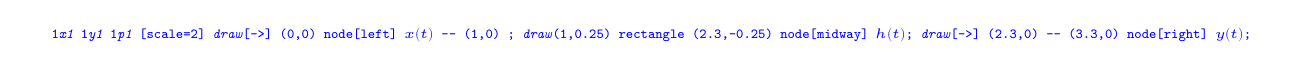
\begin{tikzpicture}[scale=2]
	\draw[->] (0,0) node[left] {$x(t)$} -- (1,0) ;
	\draw (1,0.25) rectangle (2.3,-0.25) node[midway] {$h(t)$};
	\draw[->] (2.3,0) -- (3.3,0) node[right] {$y(t)$};
	\end{tikzpicture}
\end{center}
που θεωρούμε ότι είναι χρονοαμετάβλητο, αιτιατό και ευσταθές, δηλαδή:
\begin{enumpar}
	\item \( h(t) = 0, \quad \forall t < 0 \)
	\item \( \displaystyle
	\int_{-\infty}^{\infty} \left|h(t)\right|\dif t < \infty
	 \)
	\item \(  \displaystyle
	y(t) = x(t)*h(t) = \int_{0}^{\infty}
	x(t-\lambda)h(\lambda)\dif\lambda
	= \int_{-\infty}^{t}
	x(\lambda)h(t-\lambda)\dif\lambda
	 \)
\end{enumpar}

Έστω \( \big\lbrace X(t) \big\rbrace \) με \( E\left[x(t)\right] = M \),
και:
\[
Y(t) = \int_{0}^{\infty} x(t-\lambda)h(\lambda)\dif\lambda
\]
Τότε:
\begin{align*}
	E\left[y(t)\right] &=
	E\left[\int_{0}^{\infty} x(t-\lambda) h(\lambda) \dif\lambda\right]
\end{align*}
\begin{align*}
	E\Bigg[
	\int_{t_1}^{t_2}
	\overset{\substack{\mathclap{\text{στοχαστικό}}\\\uparrow}}{x(t)}
	\underset{\substack{\downarrow\\\mathclap{\text{συνάρτηση}}}}{f(t)}
	\dif t
	\Bigg] \int_{t_1}^{t_2} E\left[x(t)\right]f(t)\dif t
\end{align*}

\begin{enumerate}
	\item \( \displaystyle
	\int_{t_1}^{t_2} E\left[\left|x(t)\right|\right]f(t)\dif t
	< \infty
	 \)
	\item \( x(t)\quad [t_1,t_2] \) πεπερασμένη
\end{enumerate}

\begin{align*}
	E\left[Y^2(t)\right] &= E\left[
	\int_{-\infty}^{\infty} (t-\lambda_1)h(\lambda_1)\dif\lambda_1
	\int_{-\infty}^{\infty} (t-\lambda_2)h(\lambda_2)\dif\lambda_2
	\right]
	\\ &= \left[
	\int_{0}^{\infty} \left[
	        E\left[
	            x(t-\lambda_1)x(t-\lambda_2)
	        \right] h(\lambda_1)h(\lambda_2)\dif\lambda_2
	    \right] \dif\lambda_1
	\right]
\end{align*}

\begin{align*}
	R_y(t_1,t_2) &= E\left[y(t_1)y(t_2)\right]
	\\ &= E\left[\int_{0}^{\infty}
	x(t_1-\lambda_1)h(\lambda_1)\dif\lambda_1
	\cdot
	\int_{0}^{\infty} x(t_2-\lambda_2)h(\lambda_2)\dif\lambda_2
	\right]
	\\ &= \int_{0}^{\infty}
	h(\lambda_1)\left[\int_{0}^{\infty}
	E\left[x(t_1-\lambda_1)x(t_2-\lambda_2)
	\right]h(\lambda_2)\dif\lambda_2
	\right]\dif\lambda_1 \\
	R_x(\tau) &= \boxed{
	    \int_{0}^{\infty}
	    \int_{0}^{\infty}
	    h(\lambda_1)h(\lambda_2)
	    R_x(\tau+\lambda_2-\lambda_1)\dif\lambda_1\dif\lambda_2
    }
\end{align*}

\subsubsection{Ετεροσυσχέτιση εξόδου-εξόδου}
\begin{align*}
	R_{xy}(t) &= E\left[x(t)Y(t+\tau)\right]
	E\left[x(t)
	\int_{0}^{\infty} x(t+\tau - \lambda)h(t)\dif\lambda
	\right]
	\\ &= E\left[
	\int_{0}^{\infty} x(t) x(t+\tau-\lambda)
	\right] h(\lambda)\dif\lambda
	\\ &= \int_{0}^{\infty} E\left[
	x(t)x(t+\tau - \lambda)
	\right] h(\lambda) \dif\lambda
	\\ &= \int_{0}^{\infty}
	R_x (\tau - \lambda)h(t)\dif\lambda
	\\
	\Aboxed{R_{xy}(\tau) &= R_x(\tau) * h(\lambda)}
\end{align*}

\subsection{Περιγραφή στο πεδίο της συχνότητας}
\begin{center}
	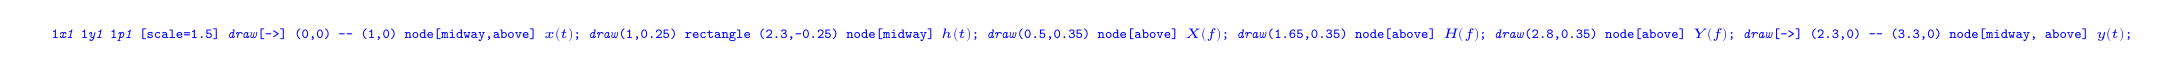
\begin{tikzpicture}[scale=1.5]
	\draw[->] (0,0) -- (1,0) node[midway,above] {$x(t)$};
	\draw (1,0.25) rectangle (2.3,-0.25) node[midway] {$h(t)$};
	\draw (0.5,0.35) node[above] {$X(f)$};
	\draw (1.65,0.35) node[above] {$H(f)$};
	\draw (2.8,0.35) node[above] {$Y(f)$};
	\draw[->] (2.3,0) -- (3.3,0) node[midway, above] {$y(t)$};
	\end{tikzpicture}
\end{center}
Είναι γνωστό ότι στο πεδίο της συχνότητας η συνέλιξη μεταφράζεται
σε πολλαπλασιασμό:
\[
X(f) = X(f)H(f)
\]

Γνωρίζουμε επίσης τη σχέση της πυκνότητας φασματικής ισχύος με τον
μετασχηματισμό Fourier:
\[
S_{\mathrm p x}  = \mathscr F \left[ R_x(\tau) \right]
\]

Σε ένα σύστημα με είσοδο \( \Big\lbrace x(t) \Big\rbrace \) και
\textbf{έξοδο \( \Big\lbrace y(t) \Big\rbrace \)}, η
\textbf{πυκνότητα φασματικής ισχύος της εξόδου} είναι:
\begin{align*}
	S_{\mathrm p y} &= \mathscr F \left[R_y(\tau)\right]
	\\ &= \int_{-\infty}^{\infty} \left[
	\int_{0}^{\infty}
	\int_{0}^{\infty}
	R_x(\tau + \lambda_2 - \lambda_1)h(\lambda_1)h(\lambda_2)
	\dif\lambda_1 \dif\lambda_2
	\right]e^{-j\omega \tau}\dif \tau
	\\ &=
	\int_{0}^{\infty}
	\int_{0}^{\infty} h(\lambda_1)h(\lambda_2)
	\left[
	\int_{-\infty}^{\infty}
	R_x \underbrace{(\tau+\lambda_2-\lambda_1)}_{t}
	\right] e^{-j\omega \tau} \dif\tau
	\\ &= \int_{0}^{\infty} \int_0^{\infty} h(\lambda_1)
	h(\lambda_2)S_{\mathrm p x}(\omega )
	e^{-j\omega (\lambda_2-\lambda_1)}
	\dif\lambda_2
	\\ &= S_{\mathrm p x}(\omega )
	\int_{0}^{\infty} h(\lambda_1)e^{j\omega \lambda_1}
	\dif\lambda_1 \int_{0}^{\infty}
	h(\lambda_2)e^{-j\omega \lambda_2}\dif\lambda_2 \\
	&= S_{\mathrm p x}(\omega ) H(-\omega ) H(\omega )
	= S_{\mathrm p x} (\omega ) \big| H(\omega ) \big|^2
\end{align*}

Δηλαδή τελικά:
\[
\boxed{
S_{\mathrm p y} (\omega ) =
\big\lvert H(\omega ) \big\rvert^2 S_{\mathrm p x}(\omega )
}
\]

Η συνάρτηση \( \big\lvert H(\omega ) \big\rvert^2 \) ονομάζεται
\textbf{συνάρτηση μεταφοράς ισχύος}.

\subsubsection{Σχέση μέσης τετραγωνικής τιμής και σφάλματος ισχύος}
\begin{align*}
	R_x(0) &= \frac{1}{2\pi} \int_{-\infty}^{\infty}
	S_{\mathrm p x}(\omega )
	\cancel{e^{-j\omega 0}}\dif \omega \\
	R_x(0) &= \frac{1}{2\pi} \int_{-\infty}^{\infty} S_{\mathrm p x}
	(\omega ) \dif (\omega ) \\
	R_x(\tau) &= E\big[ x(t)x(t+\tau) \big] \\
	R_x(0) &= E\big[ x(t)x(t) \big] = E\big[ x^2(\tau) \big] =
	\boxed{P}
\end{align*}

\begin{tikzpicture}
\fill[orange,fill opacity=.2,postaction={pattern=north east lines,opacity=.1}] plot[smooth,tension=.6] coordinates
{(-3,0.2) (-2.3,0.4) (-1.2,1.3) (1.2,1.3) (2.3,0.4) (3,0.2)}  |- (-3,0) -- cycle;

\draw (-3,0) -- (3,0) node[below] {$\omega$};
\draw (0,-0.5) -- (0,2.5) node[right] {$S_{\mathrm p x}(\omega)$};

\draw[very thick,green!60!black] plot[smooth,tension=.6] coordinates
{(-3,0.2) (-2.3,0.4) (-1.2,1.3) (1.2,1.3) (2.3,0.4) (3,0.2)};

\begin{scope}[yshift=-4cm]
\draw (-3,0) -- (3,0) node[below] {$\tau$};
\draw (0,-0.5) -- (0,2.5) node[right] {$R_{x}(\tau)$};

\draw[very thick,magenta!60!blue] plot[smooth,tension=.6] coordinates
{(-3,0.2) (-1,0.6) (0,2.2)}  plot[smooth,tension=.6] coordinates
{(0,2.2)  (1,0.6) (3,0.2)};

\filldraw[fill=black,draw=magenta!60!blue!70!black,fill opacity=.5] (0,2.2) circle(2pt) node[opacity=1,left] {$R_x(0)$};
\end{scope}
\end{tikzpicture}

\subsection{Χαρακτηριστικά στοχαστικά σήματα}
Έστω ένα στοχαστικό σήμα \( \bigg\lbrace x(t) \bigg\rbrace \) με
τυχαίες μεταβλητές \( X(t_1),\ X(t_2),\ \dots, X(t_n) \)

\subsubsection{Gaussian από κοινού κατανομή}
Δίνεται από τη σχέση:
\[
f_{x(t_1),x(t_2),\dots,x(t_n)}\big(
x(t_1),x(t_2),\dots,x(t_n)
\big) = \frac{1}{(2\pi)^{\sfrac{n}{2}\sqrt{|k|}}}
\exp\left[
-\frac{1}{2|k|} \sum_{i=1}^{n} \sum_{j=1}^{n}
\Delta_{ij} \left(
x(t_i)-\overline{x(t_i)}
\right)\left(
x(t_j)-\overline{x(t_j)}
\right)
\right]
\]
όπου \( |k| \) σημαίνει η ορίζουσα του \textbf{πίνακα συμμεταβλητότητας}:
\[
k = \left[
\begin{matrix}
k_{11} & k_{12} & \hdots & k_{1n} \\
k_{21} & k_{22} & \vdots & k_{2n} \\
\vdots & \vdots & \ddots & \vdots \\
k_{n1} & k_{n2} & \hdots & k_{nn}
\end{matrix}
\right]
\]
με στοιχεία:
\begin{align*}
	k_{ij} &= \cov\left[ x(t_i),x(t_j) \right]
	= E\left[
	\left(
	x(t_i)-\overline{x(t_i)}
	\right)\left(
	x(t_j)-\overline{x(t_j)}
	\right)
	\right] \\ &= R_x(t_i,t_j) - \overline{X(t_i)}\,\overline{X(t_j)}
	\intertext{Αν οι μέσες τιμές είναι μηδέν, φτάνουμε στον πιο απλό
	τύπο:}
    &= R_x(t_i,t_j)
\end{align*}
και \( \Delta_{ij} \) είναι η \textbf{προσημασμένη ελλάσονα} του
\( k_{ij} \) στον παραπάνω πίνακα, δηλαδή η ορίζουσα του
\( n-1 \ \times \ n-1 \) πίνακα που προκύπτει αν από τον \( k \)
αφαιρέσουμε την γραμμή και τη στήλη του \( k_{ij} \) στοιχείου,
πολλαπλασιασμένη με \( (-1)^{i+j} \):
\[
\text{Αν }
k = \left[\begin{matrix}
k_{11} & k_{12} & {\color{red} k_{13}} \\
{\color{red} k_{21}} & {\color{red} k_{22}} & {\color{red} k_{23}} \\
k_{31} & k_{32} & {\color{red} k_{33}}
\end{matrix}\right], \text{ τότε } \quad
\Delta_{23} = (-1)^{2+3}\cdot\left|\begin{matrix}
k_{11} & k_{12} \\ k_{31} & k_{32}
\end{matrix}\right|
\]

\subsubsection{Gaussian στάσιμο στοχαστικό σήμα}
Αν το σήμα είναι στάσιμο με την ευρεία έννοια, δηλαδή
\( \overline{X(t_i)} =  \) σταθερό και \( R_x(t_i,t_j)
= R_x(t_i-t_j)
\):

Παρατηρούμε ότι το στάσιμο γκαουσιανό σήμα δεν μεταβάλλεται όταν
μετατοπίζεται στο χρόνο, επομένως είναι και στάσιμο με την αυστηρή
έννοια. Όταν επίσης ένα gaussian στοχαστικό σήμα είναι είσοδος σε
ένα γραμμικό σύστημα, η έξοδός του είναι επίσης gaussian. Τα γκαουσιανά
σήματα είναι χρήσιμα επειδή με αυτά συχνά μοντελοποιούμε τον θόρυβο.

\subsubsection{Λευκός θόρυβος}
\begin{center}
	\begin{tikzpicture}[scale=1]
	\draw[gray,->] (0,0) -- (7.2,0) node[below right] {$t$};
	\draw[gray,->] (0,-2) -- (0,2);

	\draw[black] plot[domain=0.01:7,smooth,tension=.1,samples=100] (\x,rand);
	\end{tikzpicture}
\end{center}

AWGN (Additive White Gaussian Noise) - προέρχεται από την κίνηση
των ηλεκτρονίων στους ηλεκτροφόρους αγωγούς, εμφανίζεται σε διόδους
p-n, κεραίες, στον κοσμικό θόρυβο, \dots

Χαρακτηριστικό του είναι η πυκνότητα φασματικής ισχύος, που είναι
σταθερή από το \( -\infty \) μέχρι το \( \infty \):
\[
\underline{S_{\mathrm p x}(\omega ) = S_0}
\]

\begin{tikzpicture}[scale=1]
\draw (-3,0) -- (3,0) node[below right] {$\omega$};
\draw[->] (0,-1) -- (0,2) node[left] {$S_{\mathrm p x}(\omega)$};
\fill[orange,postaction={pattern=north east lines,opacity=.3},fill opacity=.5] (1,0) rectangle ++(0.4,1);
\draw (1,0) -- ++(0,1) (1.4,0) -- ++(0,1) (1.2,0) node[below] {$\dif x$};

\draw[very thick,green!60!black,blur shadow,shadow xshift=0cm,shadow yshift=-0.3mm] (-3,1) -- (3,1);

\draw (0,1) node[above right] {$S_0$};
\end{tikzpicture}

Αυτό σημαίνει ότι όλες οι συχνότητες συμμετέχουν με το ίδιο μερίδιο
ισχύος στην κατασκευή του σήματος (το όνομα "\emph{λευκός}"
παραπέμπει στο φάσμα του Νεύτωνα, και στην ανάμιξη όλων των χρωμάτων,
που δίνει λευκό φως).

Ισχύει:
\[
E\left[x^2(t)\right] = \frac{1}{2\pi}
\int_{-\infty}^{\infty} S_{\mathrm p x}(\omega )
\dif \omega = \infty
\]
Δηλαδή ο ιδανικός θόρυβος έχει άπειρη ενέργεια! (Στην πραγματικότητα
η πυκνότητα φασματικής ενέργειας αρχίζει και μειώνεται μετά τα
\( 2000 \si{\giga\hertz} \), και δεν μπορεί να κατασκευαστεί συσκευή
με μεγάλο εύρος φάσματος ώστε να παράξει άπειρη ισχύ).

Για τη συνάρτηση αυτοσυσχέτισης ισχύει:
\[
R_{x}(\tau) = S_0\delta(\tau)
\]

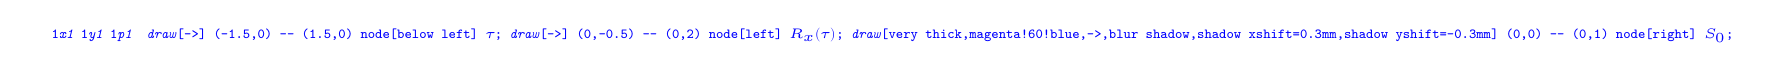
\begin{tikzpicture}
\draw[->] (-1.5,0) -- (1.5,0) node[below left] {$\tau$};
\draw[->] (0,-0.5) -- (0,2) node[left] {$R_x(\tau)$};

\draw[very thick,magenta!60!blue,->,blur shadow,shadow xshift=0.3mm,shadow yshift=-0.3mm] (0,0) -- (0,1) node[right] {$S_0$};
\end{tikzpicture}

Αυτό σημαίνει ότι η τιμή του σήματος κάθε στιγμή, δεν εξαρτάται καθόλου
από οποιαδήποτε άλλη τιμή, δηλαδή το σήμα είναι εντελώς τυχαίο.

\begin{tikzpicture}[scale=1]
\draw[->] (-1,0) -- (4.2,0) node[below] {$t$};
\draw[->] (0,-1) -- (0,2) node[left] {$\underset{\text{noise}}{n(t)}$};

\draw[thick,blue!60!black,mark position=0.2(a),mark position=0.7(b)]
plot [smooth, tension=0.4, domain=0:4, samples=20] (\x,{0.4+0.8*rand});

\draw[dashed] (a) -- (a |- 0,0) node[below] {$t_1$};
\draw[dashed] (b) -- (b |- 0,0) node[below] {$t_2$};
\end{tikzpicture}

\subsubsection{Εφαρμογή}
Αν τον προηγούμενο με άπειρο εύρος μπάντας λευκό θόρυβο τον περάσουμε
μέσα από ένα πεπερασμένου εύρους συχνοτήτων σύστημα:

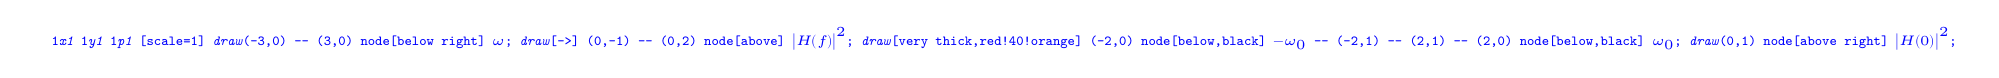
\begin{tikzpicture}[scale=1]
\draw (-3,0) -- (3,0) node[below right] {$\omega$};
\draw[->] (0,-1) -- (0,2) node[above] {$\big\lvert H(f)\big\rvert^2$};

\draw[very thick,red!40!orange]
(-2,0) node[below,black] {$-\omega_0$} -- (-2,1) -- (2,1) -- (2,0) node[below,black] {$\vphantom{-}\omega_0$};

\draw (0,1) node[above right] {$\big\lvert H(0)\big\rvert^2$};
\end{tikzpicture}
\[
S_{\mathrm p x}(\omega )\left|H(\omega )\right|^2
\]
και έχουμε την έξοδο:

\begin{tikzpicture}[scale=1]
\draw (-3,0) -- (3,0) node[below right] {$\omega$};
\draw[->] (0,-1) -- (0,2) node[above] {$S_{\mathrm p}\big\lvert H(f)\big\rvert^2$};

\draw[very thick,green!60!black]
(-2,0) node[below,black] {$-\omega_0$} -- (-2,1.2) -- (2,1.2) -- (2,0) node[below,black] {$\vphantom{-}\omega_0$};

\draw (0,1.2) node[above right] {$S_0$};
\end{tikzpicture}
\[
S_{\mathrm p y}(\omega ) = \begin{cases}
S_0' \quad & |\omega | \leq \omega_0 \\
0 \quad & \text{αλλού}
\end{cases}
\]
που δεν είναι λευκός θόρυβος, αλλά έχει "\emph{χρωματιστεί}", η
συνάρτηση αυτοσυσχέτισης είναι (\( \mathscr F^{-1} \)):
\[
R_x(\tau) = \frac{\omega_0 S_0'}{\pi}
\underbrace{\frac{\sin(\omega_0\tau)}{\omega_0\tau}}_{
	\sinc(\omega_0 t)}
\]
\begin{tikzpicture}[scale=1.2]
\draw[->] (0,-0.5) -- (0,1.5) node[right] {$R_x(\tau)$};
\draw[->] (-2.5,0) -- (2.5,0);

\draw[very thick,xscale=0.5,samples=200,domain=-5:5,smooth,variable=\x,magenta!60!blue]
plot ({\x},{sinc(pi*\x)});

\foreach \x in {-2,-1.5,...,2} {
   	\filldraw[fill=magenta!50!white,fill opacity=.5] (\x,0) circle (1.5pt);
}
\end{tikzpicture}

δηλαδή στην πραγματικότητα, οι εναλλαγές στον θόρυβο είναι ομαλές,
και δεν μπορούν να παίρνουν οποιεσδήποτε τιμές.

\begin{tikzpicture}
\draw (-3,0) -- (3,0);
\draw (0,-0.5) -- (0,2.5);

\draw[very thick] (1,0) -- ++(0,1.5) --++(1,0) --++(0,-1.5);
\draw[very thick,green!50!black] (1.35,0) -- ++(0,1.5) --++(0.3,0) --++(0,-1.5);
\draw (1.5,-0.1) node[below] {$f_1$} -- (1.5,0.1);
\draw[->,thick,green!50!black,opacity=.8] (2-0.07,0.75) -- (1.65+0.07,0.75);
\draw[->,thick,green!50!black,opacity=.8] (1+0.07,0.75) -- (1.35-0.07,0.75);

\begin{scope}[xscale=-1]
\draw[very thick] (1,0) -- ++(0,1.5) --++(1,0) --++(0,-1.5);
\draw[very thick,green!50!black] (1.35,0) -- ++(0,1.5) --++(0.3,0) --++(0,-1.5);
\draw (1.5,-0.1) node[below] {$-f_1$} -- (1.5,0.1);
\draw[->,thick,green!50!black,opacity=.8] (2-0.07,0.75) -- (1.65+0.07,0.75);
\draw[->,thick,green!50!black,opacity=.8] (1+0.07,0.75) -- (1.35-0.07,0.75);
\end{scope}
\end{tikzpicture}

Όσο μικραίνει το εύρος ζώνης και τείνει στο 0 (ώση), ο
\( \mathscr F^{-1} \)
γίνεται ένα συνημίτονο, δηλαδή αυξάνεται η αυτοσυσχέτιση.

\end{document}
